% % Preamble BEGINN %%%%%%%%%%%%%%%%%%%%%%%%%%%%%%%%%%%%%%%%%%%%%%%%%%%%%%%%%

%%% Preamble (Dokumentenklasse)
% ------------------------------------------------------------------------
% LaTeX - Preambel ******************************************************
% ------------------------------------------------------------------------
% Dokumentklasse (Koma Script)
% ------------------------------------------------------------------------
% basiernd auf www.matthiaspospiech.de/latex/vorlagen Diplomarbeit kompakt
% ========================================================================
\documentclass[%
   %draft,            % Entwurfsstadium
   final,             % fertiges Dokument
   11pt,              % Schriftgroesse der Grundschrift
   bigheadings,       % gro�e �berschriften
   ngerman,           % wird an andere Pakete weitergereicht
   a4paper,           % Papierformat
   BCOR5mm,          % Bindekorrektur: Zus�tzlicher Rand auf der Innenseite
   DIV14,            % Seitengr��e (siehe Koma Skript Dokumentation !)
   1.1headlines,     % Zeilenanzahl der Kopfzeilen
   pagesize,         % Schreibt die Papiergroesse in die Datei.
   oneside,          % Einseitiges Layout
%   twoside,          % Zweiseitiges Layout
   openright,        % Kapitel beginnen immer auf der rechten Seite
   titlepage,        % Titel als einzelne Seite ('titlepage' Umgebung)  
   headsepline,      % Linie unter Kolumnentitel ()
%   plainheadsepline, % Linie unter Kolumnentitel () plain Seitenstil
   nochapterprefix,  % keine Ausgabe von 'Kapitel:'
   bibtotoc,         % Bibliographie ins TOC
%	bibtotocnumbered, % Bibliographie ins TOC mit Kapitelnummer
   tocindent,        % eingereuckte Gliederung
   listsindent,      % eingereuckte LOT, LOF
   pointlessnumbers, % �berschriftnummerierung ohne Punkt, siehe DUDEN !
   cleardoubleempty, % Leere linke Seite bei Zweiseitenlayout vor Kapitel
   fleqn,            % Formeln werden linksbuendig angezeigt
%   parindent,        % Absatz mit Einzug (Standard)
   halfparskip,      % Absatz halbe Zeile Abstand
%   parskip,          % Absatz ganze Zeile Abstand
]{scrbook}%     Klassen: scrartcl, scrreprt, scrbook


%%% Alle Namen usw. im Titel und im hyperref-Paket
% ------------------------------------------------------------------------
% LaTeX - Preambel ******************************************************
% ------------------------------------------------------------------------
% pre-work
% ========================================================================
% % ToDo kennzeichnen
\newcommand{\workTodo}[1]{\textcolor{red}{todo: #1}}

% % F�r Datum und Zeit in Fusszeile
% % !!!Inhalt bei Fertigstellung der Arbeit l�schen
\newcommand{\workMarkDateTime}{\workTodo{\today{} - \thistime\ Uhr}}

% % Alle Namen werden im Titel und im hyperref-Paket eingetragen
% % !!! Ueberall f�r <Wert> das Entsprechende eintragen

 % <Typ> Studienarbeit, Dipolmarbeit, Studienarbeit oder Bachlor-Abschlussarbeit
\newcommand{\workTyp}{\workTodo{<Typ>}\xspace}

 % <Titel> der Arbeit
\newcommand{\workTitel}{\workTodo{<Titel>}}

 % <Studiengang> z.B. Kommunikationstechnik
\newcommand{\workStudiengang}{\workTodo{<Studiengang>}\xspace}

% <Semester> mit Jahr z.B. Sommersemester 2008  
\newcommand{\workSemester}{\workTodo{<Semester>}\xspace}

% <Name> des Studenten
\newcommand{\workNameStudent}{\workTodo{<Name>}\xspace}

% <Pruefer> Name des pr�fenden (betreuenden) Professor an der Hochschule
\newcommand{\workPruefer}{\workTodo{<Pruefer>}\xspace} 


% %%% Nur bei Abschluss-Arbeiten

% <Datum> der Abgabe der Arbeit (Eidesstatliche Erkl�rung)
\newcommand{\workDatum}{\today\xspace}

% <Zweitpr�fer>
\newcommand{\workZweitPruefer}{\workTodo{<Zweitpr�fer>}\xspace}

% <Zeitraum>
\newcommand{\workZeitraum}{\workTodo{<Zeitraum>}\xspace}


% %%% Nur bei Industrie-Arbeiten:

% <Firma>
\newcommand{\workFirma}{\workTodo{<Firma>}\xspace}

% <Betreuer in der Firma>
\newcommand{\workBetreuer}{\workTodo{<Betreuer in der Firma>}\xspace}

% Firmenlogo Name hier anpassen, Gr��e (wenn m�glich) nicht �ndern
\newcommand{\workFirmenLogo}{
\includegraphics[width=5cm]{fig/aa-titel/Bosch_4C_S}} 


%%% Preamble (Pakete)
% ------------------------------------------------------------------------
% LaTeX - Preambel ******************************************************
% ------------------------------------------------------------------------
% Packages
% ------------------------------------------------------------------------
% basiernd auf www.matthiaspospiech.de/latex/vorlagen Diplomarbeit kompakt
% ========================================================================

% Inhalt:
% 1. Einige Pakete muessen unbedingt vor allen anderen geladen werden
% 2. Fonts Fonts Fonts
% 3. Math Packages
% 4. Symbole
% 5. text related packages
% 6. Pakete zum Zitieren
% 7. PDF related packages
% 8. Tables (Tabular)
% 9. figures and placement
% 10. verbatim packages
% 11. science packages
% 12. layout packages

% ~~~~~~~~~~~~~~~~~~~~~~~~~~~~~~~~~~~~~~~~~~~~~~~~~~~~~~~~~~~~~~~~~~~~~~~~
% Encoding der Dateien (sonst funktionieren Umlaute nicht)
% Empfohlen latin1, da einige Pakete mit utf8 Zeichen nicht
% funktionieren, z.B: listings, soul.

\usepackage[latin1]{inputenx} % ISO-8859-1
%\usepackage[ansinew]{inputenx} % Windows-Standard (CP1252) (baut auf ISO 8859-1 und ISO 8859-15 auf)
%\usepackage[utf8]{inputenc}

% ~~~~~~~~~~~~~~~~~~~~~~~~~~~~~~~~~~~~~~~~~~~~~~~~~~~~~~~~~~~~~~~~~~~~~~~~
% 1. Einige Pakete muessen unbedingt vor allen anderen geladen werden
% ~~~~~~~~~~~~~~~~~~~~~~~~~~~~~~~~~~~~~~~~~~~~~~~~~~~~~~~~~~~~~~~~~~~~~~~~
%
\usepackage{xspace} % Define commands that don't eat spaces.
\usepackage{ifpdf} % Fuer Pakete/Paketoptionen, die nur fuer pdf benoetigt werden \ifpdf \else \fi
\usepackage{calc} % Calculation with LaTeX
\usepackage[ngerman]{babel} % Languagesetting
\usepackage[table]{xcolor} % Farben
\usepackage[]{graphicx} % Bilder
%\usepackage{epstopdf} % If an eps image is detected, epstopdf is automatically called to convert it to pdf format.
\usepackage[]{amsmath} % Amsmath - Mathematik Basispaket
\usepackage{ragged2e} % Besserer Flatternsatz (Linksbuendig, statt Blocksatz)

% ~~~~~~~~~~~~~~~~~~~~~~~~~~~~~~~~~~~~~~~~~~~~~~~~~~~~~~~~~~~~~~~~~~~~~~~~
% 2. Fonts Fonts Fonts
% ~~~~~~~~~~~~~~~~~~~~~~~~~~~~~~~~~~~~~~~~~~~~~~~~~~~~~~~~~~~~~~~~~~~~~~~~

\usepackage[T1]{fontenc} % T1 Schrift Encoding (notwendig f�r die meisten Type 1 Schriften)
\usepackage{textcomp}	 % Zusatzliche Symbole (Text Companion font extension)

% Alle Schriften die hier angegeben sind sehen im PDF richtig aus.
% Die LaTeX Standardschrift ist die Latin Modern (lmodern Paket).
% If Latin Modern is not available for your distribution you must install the
% package cm-super instead. Otherwise your fonts will look horrible in the PDF

% DO NOT LOAD ae-Package for the font !

%% - Latin Modern
\usepackage{lmodern}
%% -------------------
%
% % - Times, Helvetica, Courier (Word Standard...)
%\usepackage{mathptmx}
%\usepackage[scaled=.90]{helvet}
%\usepackage{courier}
% % -------------------
%%
%% - Palantino , Helvetica, Courier
%\usepackage{mathpazo}
%\usepackage[scaled=.95]{helvet}
%\usepackage{courier}
%% -------------------
%
%% - Bera Schriften
%\usepackage{bera}
%% -------------------
%
%% - Charter, Bera Sans
%\usepackage{charter}\linespread{1.05}
%\renewcommand{\sfdefault}{fvs}


% ~~~~~~~~~~~~~~~~~~~~~~~~~~~~~~~~~~~~~~~~~~~~~~~~~~~~~~~~~~~~~~~~~~~~~~~~
% 3. Math Packages
% ~~~~~~~~~~~~~~~~~~~~~~~~~~~~~~~~~~~~~~~~~~~~~~~~~~~~~~~~~~~~~~~~~~~~~~~~

\usepackage[fixamsmath,disallowspaces]{mathtools} % Erweitert amsmath und behebt einige Bugs
\usepackage{fixmath}
\usepackage[all,warning]{onlyamsmath} % Warnt bei Benutzung von Befehlen die mit amsmath inkompatibel sind.
\usepackage{icomma} % Erlaubt die Benutzung von Kommas im Mathematikmodus

% ~~~~~~~~~~~~~~~~~~~~~~~~~~~~~~~~~~~~~~~~~~~~~~~~~~~~~~~~~~~~~~~~~~~~~~~~
% 4. Symbole
% ~~~~~~~~~~~~~~~~~~~~~~~~~~~~~~~~~~~~~~~~~~~~~~~~~~~~~~~~~~~~~~~~~~~~~~~~
\usepackage{amssymb}
%\usepackage{wasysym}
%\usepackage{marvosym}
%\usepackage{pifont}

% ~~~~~~~~~~~~~~~~~~~~~~~~~~~~~~~~~~~~~~~~~~~~~~~~~~~~~~~~~~~~~~~~~~~~~~~~
% 5. text related packages
% ~~~~~~~~~~~~~~~~~~~~~~~~~~~~~~~~~~~~~~~~~~~~~~~~~~~~~~~~~~~~~~~~~~~~~~~~

\usepackage{url} % Setzen von URLs. In Verbindung mit hyperref sind diese auch aktive Links.
\usepackage[stable,perpage, ragged,  multiple]{footmisc} % Fussnoten
\usepackage[ngerman]{varioref} % Intelligente Querverweise
\usepackage{enumitem} % Listen

% ~~~~~~~~~~~~~~~~~~~~~~~~~~~~~~~~~~~~~~~~~~~~~~~~~~~~~~~~~~~~~~~~~~~~~~~~
% 6. Pakete zum Zitieren
% ~~~~~~~~~~~~~~~~~~~~~~~~~~~~~~~~~~~~~~~~~~~~~~~~~~~~~~~~~~~~~~~~~~~~~~~~

\usepackage[babel, german=quotes, english=british, french=guillemets]{csquotes} % clever quotations
\SetBlockThreshold{2} % Anzahl von Zeilen
\newenvironment{myquote}%
          {\begin{quote}\small}%
          {\end{quote}}%
\SetBlockEnvironment{myquote}
\usepackage[numbers]{natbib}
\bibliographystyle{abbrvnat}

% ~~~~~~~~~~~~~~~~~~~~~~~~~~~~~~~~~~~~~~~~~~~~~~~~~~~~~~~~~~~~~~~~~~~~~~~~
% 7. PDF related packages
% ~~~~~~~~~~~~~~~~~~~~~~~~~~~~~~~~~~~~~~~~~~~~~~~~~~~~~~~~~~~~~~~~~~~~~~~~

\ifpdf % Wenn als PDF ausgegeben wird
\usepackage{pdfpages} % pdf-Seiten einbinden
\usepackage[pdftex]{hyperref} % PDF Option in Hyperref
\else
\usepackage[dvipdfm]{hyperref}
\fi

%%% Doc: ftp://tug.ctan.org/pub/tex-archive/macros/latex/contrib/pdfpages/pdfpages.pdf
%\usepackage{pdfpages} % Include pages from external PDF documents in LaTeX documents

%%% Doc: ftp://tug.ctan.org/pub/tex-archive/macros/latex/contrib/hyperref/doc/manual.pdf
\hypersetup{
          pdfhighlight = /O,	         % Visualisierung beim anklicken von Links
% Farben fuer die Links
   colorlinks=true,	        % Links erhalten Farben statt Kaestchen
   urlcolor=darkblue,    % \href{...}{...} external (URL)
   filecolor=darkblue,  % \href{...} local file
   linkcolor=darkblue,  % \ref{...} and \pageref{...}
          citecolor =darkblue,    % Literaturverzeichnis
   % Links
   raiselinks=true,			 % calculate real height of the link
   breaklinks,	        % Links bestehen bei Zeilenumbruch
%   backref=page,	         % Backlinks im Literaturverzeichnis (section, slide, page, none)
%   pagebackref=true,        % Backlinks im Literaturverzeichnis mit Seitenangabe
   verbose,
%   hyperindex=true,         % backlinkex index
   linktocpage=true,        % Inhaltsverzeichnis verlinkt Seiten
%   hyperfootnotes=false,	% Keine Links auf Fussnoten
   % Bookmarks
%   bookmarks=true,	         % Erzeugung von Bookmarks fuer PDF-Viewer
   bookmarksopenlevel=1,    % Gliederungstiefe der Bookmarks
   bookmarksopen=true,      % Expandierte Untermenues in Bookmarks
   bookmarksnumbered=true,  % Nummerierung der Bookmarks
   bookmarkstype=toc,       % Art der Verzeichnisses
   % Anchors
   plainpages=false,        % % Make page anchors using the formatted form of the page number. With this option, hyperref writes different anchors for pages �ii� and �2�. (If the option is set �true� � the default � hyperref writes page anchors as the arabic form of the absolute page number, rather than the formatted form.)
   % hypertexnames=false,
   pageanchor=true,	        % Pages are linkable
   % PDF Informationen
   pdftitle={\workTyp: \workTitel},	        % Titel
   pdfauthor={\workNameStudent},	    % Autor
   pdfcreator={LaTeX, hyperref, KOMA-Script}, % Ersteller
   %pdfproducer={pdfeTeX 1.10b-2.1} %Produzent
   pdfstartview=FitH,       % Dokument wird Fit Width geaefnet
   pdfpagemode=UseOutlines, % Bookmarks im Viewer anzeigen
%   pdfpagelabels=true,      % set PDF page labels
}

% ~~~~~~~~~~~~~~~~~~~~~~~~~~~~~~~~~~~~~~~~~~~~~~~~~~~~~~~~~~~~~~~~~~~~~~~~
% 8. Tables (Tabular)
% ~~~~~~~~~~~~~~~~~~~~~~~~~~~~~~~~~~~~~~~~~~~~~~~~~~~~~~~~~~~~~~~~~~~~~~~~

\usepackage{booktabs}
\usepackage{tabularx} % tabularx nach hyperref laden
\usepackage{multirow}
\usepackage{longtable}

% ~~~~~~~~~~~~~~~~~~~~~~~~~~~~~~~~~~~~~~~~~~~~~~~~~~~~~~~~~~~~~~~~~~~~~~~~
% 9. figures and placement
% ~~~~~~~~~~~~~~~~~~~~~~~~~~~~~~~~~~~~~~~~~~~~~~~~~~~~~~~~~~~~~~~~~~~~~~~~

%% Bilder und Graphiken ==================================================

\usepackage{float}	% Stellt die Option [H] fuer Floats zur Verfgung
\usepackage{flafter} % Floats immer erst nach der Referenz setzen
\usepackage{subfig} % Layout wird weiter unten festgelegt !
\usepackage{wrapfig} % Bilder von Text Umfliessen lassen

\usepackage{placeins} % Alle Floats bis \FloatBarrier ausgeben

% Make float placement easier
\renewcommand{\floatpagefraction}{.75} % vorher: .5
\renewcommand{\textfraction}{.1}       % vorher: .2
\renewcommand{\topfraction}{.8}        % vorher: .7
\renewcommand{\bottomfraction}{.5}     % vorher: .3
\setcounter{topnumber}{3}	         % vorher: 2
\setcounter{bottomnumber}{2}	         % vorher: 1
\setcounter{totalnumber}{5}	         % vorher: 3
\usepackage{tikz}
%\usetikzlibrary{shapes, snakes, spy, positioning}
\def\layersep{2.5cm}


% ~~~~~~~~~~~~~~~~~~~~~~~~~~~~~~~~~~~~~~~~~~~~~~~~~~~~~~~~~~~~~~~~~~~~~~~~
% 10. verbatim packages
% ~~~~~~~~~~~~~~~~~~~~~~~~~~~~~~~~~~~~~~~~~~~~~~~~~~~~~~~~~~~~~~~~~~~~~~~~

%%% Doc: ftp://tug.ctan.org/pub/tex-archive/macros/latex/contrib/upquote/upquote.sty
\usepackage{upquote} % Setzt "richtige" Quotes in verbatim-Umgebung

%%% Doc: No Documentation
% \usepackage{verbatim} % Reimplemntation of the original verbatim

%%% Doc: http://www.cs.brown.edu/system/software/latex/doc/fancyvrb.pdf
% \usepackage{fancyvrb} % Superior Verbatim Class

%% Listings Paket ------------------------------------------------------
%%% Doc: ftp://tug.ctan.org/pub/tex-archive/macros/latex/contrib/listings/listings-1.3.pdf
\usepackage{listings}

\lstset{
basicstyle =\ttfamily\color{black}\small, % Standardschrift
keywordstyle =, % \bfseries\color{blue}	  % Schl�sselwort-Style
%identifierstyle =\underbar,
commentstyle =\color{teal},
stringstyle =\itshape,
numbers = left,			  % Ort der Zeilennummern
numberstyle =\tiny\color{black},	   % Stil der Zeilennummern
numbers = left,			  % Ort der Zeilennummern
tabsize=2,			  % Groesse von Tabs
breaklines,			  % Zeilen werden Umgebrochen
breakatwhitespace,			  % An Leerzeichen umbrechen
%showspaces=true,			  % Leerzeichen anzeigen
backgroundcolor=\color{lightgray},	  % % Hintergrundfarbe der Listings
}
 \lstloadlanguages{% Check Dokumentation for further languages ...
%	[Visual]Basic
         [AlLaTeX]TeX,
         %Pascal
         %C
         %C++
         %XML
         %HTML
 }

%%% Doc: ftp://tug.ctan.org/pub/tex-archive/macros/latex/contrib/examplep/eurotex_2005_examplep.pdf
% LaTeX Code und Ergebnis nebeneinander darstellen
%\usepackage{examplep}


% ~~~~~~~~~~~~~~~~~~~~~~~~~~~~~~~~~~~~~~~~~~~~~~~~~~~~~~~~~~~~~~~~~~~~~~~~
% 11. science packages
% ~~~~~~~~~~~~~~~~~~~~~~~~~~~~~~~~~~~~~~~~~~~~~~~~~~~~~~~~~~~~~~~~~~~~~~~~

\usepackage[squaren]{SIunits}

% ~~~~~~~~~~~~~~~~~~~~~~~~~~~~~~~~~~~~~~~~~~~~~~~~~~~~~~~~~~~~~~~~~~~~~~~~
% 12. layout packages
% ~~~~~~~~~~~~~~~~~~~~~~~~~~~~~~~~~~~~~~~~~~~~~~~~~~~~~~~~~~~~~~~~~~~~~~~~

%% Zeilenabstand =========================================================
%
%%% Doc: ftp://tug.ctan.org/pub/tex-archive/macros/latex/contrib/setspace/setspace.sty
\usepackage{setspace}
%\doublespace	        % 2-facher Abstand
%\onehalfspace	  % 1,5-facher Abstand
% hereafter load 'typearea' again

%% Seitenlayout ==========================================================
%
% Layout mit 'typearea'
\typearea[current]{last}
\raggedbottom     % Variable Seitenhoehen zulassen


%% Kopf und Fusszeilen====================================================
%%% Doc: ftp://tug.ctan.org/pub/tex-archive/macros/latex/contrib/koma-script/scrguide.pdf
\usepackage[%
   automark,	 % automatische Aktualisierung der Kolumnentitel
   nouppercase,	 % Grossbuchstaben verhindern
]{scrlayer-scrpage}

\usepackage{scrtime} % Zeit
%\usepackage{scrdate} % Datum

\pagestyle{scrheadings} % Seite mit Headern
%\pagestyle{scrplain} % Seiten ohne Header
%\pagestyle{empty} % Seiten ohne Header

% loescht voreingestellte Stile
\clearmainofpairofpagestyles
\clearplainofpairofpagestyles
%
% [scrplain]{scrheadings}

% %%% Kopfzeile
% einseitig: Bei einseitigem Layout, nur folgende Zeilen verwenden !!!
\ihead[]{\leftmark} % links: Kapitel
 %\chead[\pagemark]{\pagemark} % mitte:
\ohead[]{\rightmark} % rechts: Section

% %zweiseitig: Bei zweiseitigem Layout, nur folgende Zeilen verwenden !!!
%\ihead[]{} % innen
% % \chead[\pagemark]{\pagemark} % mitte:
%\ohead[]{\headmark} % aussen: Kapitel (linke Seite) und Section (rechte Seite)
%
% %%% Fusszeile
\ifoot[\workMarkDateTime]{\workMarkDateTime} % innen:
%\cfoot[\pagemark]{\pagemark} % mitte:
\ofoot[\pagemark]{\pagemark} % aussen: Seitenzahl

% Angezeigte Abschnitte im Header
\automark[section]{chapter} % Inhalt von [\rightmark]{\leftmark}
%
% Linie zwischen Kopf und Textk�rper
\setheadsepline{.4pt}[\color{black}]

%% Fussnoten =============================================================
% Keine hochgestellten Ziffern in der Fussnote (KOMA-Script-spezifisch):
\deffootnote{1.5em}{1em}{\makebox[1.5em][l]{\thefootnotemark}}
\addtolength{\skip\footins}{\baselineskip} % Abstand Text <-> Fussnote
\setlength{\dimen\footins}{10\baselineskip} % Beschraenkt den Platz von Fussnoten auf 10 Zeilen
\interfootnotelinepenalty=10000 % Verhindert das Fortsetzen von
                                % Fussnoten auf der gegen�berligenden Seite

%% Schriften (Sections )==================================================

% -- Koma Schriften --
\newcommand\SectionFontStyle{\sffamily}

\setkomafont{chapter}{\huge\SectionFontStyle}    % Chapter
\setkomafont{sectioning}{\SectionFontStyle} %  % Titelzeilen % \bfseries

\setkomafont{pagenumber}{\bfseries\SectionFontStyle} % Seitenzahl
\setkomafont{pagehead}{\small\sffamily}	       % Kopfzeile

\setkomafont{descriptionlabel}{\itshape}        % Stichwortliste
%
\renewcommand*{\raggedsection}{\raggedright} % Titelzeile linksbuendig, haengend
%

%% Captions (Schrift, Aussehen) ==========================================

%%% Doc: ftp://tug.ctan.org/pub/tex-archive/macros/latex/contrib/caption/caption.pdf
\usepackage{caption}
% Aussehen der Captions
\captionsetup{
   margin = 10pt,
   font = {small,rm},
   labelfont = {small,bf},
   format = plain, % oder 'hang'
   indention = 0em,	 % Einruecken der Beschriftung
   labelsep = colon, %period, space, quad, newline
   justification = RaggedRight, % justified, centering
   singlelinecheck = true, % false (true=bei einer Zeile immer zentrieren)
   position = bottom %top
}
%%% Bugfix Workaround
\DeclareCaptionOption{parskip}[]{}
\DeclareCaptionOption{parindent}[]{}

% Aussehen der Captions fuer subfigures (subfig-Paket)
\captionsetup[subfloat]{%
   margin = 10pt,
   font = {small,rm},
   labelfont = {small,bf},
   format = plain, % oder 'hang'
   indention = 0em,	 % Einruecken der Beschriftung
   labelsep = space, %period, space, quad, newline
   justification = RaggedRight, % justified, centering
   singlelinecheck = true, % false (true=bei einer Zeile immer zentrieren)
   position = bottom, %top
   labelformat = parens % simple, empty % Wie die Bezeichnung gesetzt wird
 }

%% Inhaltsverzeichnis (Schrift, Aussehen) sowie weitere Verzeichnisse ====

\setcounter{secnumdepth}{2}	 % Abbildungsnummerierung mit groesserer Tiefe
\setcounter{tocdepth}{2}		 % Inhaltsverzeichnis mit groesserer Tiefe
%

% Farben ================================================================
% Farben fuer die Links im PDF

\definecolor{green}{rgb}{0,0.5,0} % gr�n
\definecolor{brown}{rgb}{0.6,0,0} % braun
\definecolor{darkblue}{rgb}{0,0,.5} % dunkelblau
\definecolor{lightblue}{rgb}{0.8,0.85,1} % hellblau
% Farben fuer Listings
\colorlet{stringcolor}{green!40!black!100}
\colorlet{commencolor}{blue!0!black!100}


% Auszufuehrende Befehle  ------------------------------------------------

%\listfiles
%------------------------------------------------------------------------


%%% Neue Befehle
% ------------------------------------------------------------------------
% LaTeX - Preambel ******************************************************
% ------------------------------------------------------------------------
% pre-newcommands
% ========================================================================
% ---- Hervorhebungen
% demo.tex Hervorhebungen
\newcommand{\env}[1]{\texttt{#1}}
\newcommand{\command}[1]{\texttt{#1}}
\newcommand{\package}[1]{\texttt{\itshape#1}}
\newcommand{\engl}[1]{(engl: \textit{#1})\xspace}
\newcommand{\mathbfit}[1]{\mathbf{\mathit{#1}}}

% todo
\newcommand{\todo}[1]{{\color{red}#1}\xspace}
\newcommand{\bv}{\todo{BV}} % Begriffsverzeichnis
\newcommand{\kap}{\todo{Kp}} % Kapitel

% TeX
\newcommand{\latex}{\LaTeX\xspace}
\newcommand{\tex}{\TeX\xspace}
\newcommand{\miktex}{MiK\TeX\xspace}
\newcommand{\bibtex}{Bib\TeX\xspace}

\newcommand{\led}{LEd\xspace}

\newcommand{\koma}{KOMA-Script\xspace}

% Internetseite
\newcommand{\www}[1]{\href{http://#1}{#1}}
\newcommand{\wwwhttp}[1]{\href{#1}{#1}}
\newcommand{\wwwlink}[1]{\footnote{\www{#1}}}

% Textauszeichnungen
\newcommand{\textemph}[1]{\textit{#1}} % Hervorheben
\newcommand{\textemphs}[1]{\textbf{#1}} % Hervorheben fett
\newcommand{\textqu}[1]{\enquote{#1}} % Anf�hrungszeichen
\newcommand{\tshortcut}[1]{\textit{#1}}
\newcommand{\textbutton}[1]{\textit{#1}}
\newcommand{\textmenu}[1]{\textit{#1}}
\newcommand{\textlst}[1]{\texttt{#1}} % Listings im Text
%\newcommand{\textcode}[1]{\texttt{#1}\xspace} % 
%\newcommand{\texttask}[1]{\textit{#1}}


% ---- Abkuerzungen
\newcommand{\zB}{\mbox{z.\,B.}\xspace}
\newcommand{\ua}{\mbox{u.\,a.}\xspace}
\newcommand{\dah}{\mbox{d.\,h.}\xspace}
\newcommand{\Dah}{\mbox{D.\,h.}\xspace}
\newcommand{\uAe}{\mbox{u.\,�.}\xspace}

% ---- Listings
\newcommand{\lst}[1]{\lstinline$#1$} % geht nicht

\newcommand{\lstergibt}[1]{Ergibt:\newline{}}
%%%%%%%%%%%%%%%%%%%%%%%%%%%%%%%%%%%%%%%%%%%%%%%%%%%%%%%%%%%%%%%%%%%%%%%%%%%%%%
% ---- Querverweise
\newcommand{\refs}[1]{\mbox{(s.~\autoref{#1})}\xspace}
\newcommand{\refsauch}[1]{(s. auch \autoref{#1})\xspace}
\newcommand{\refn}[1]{\mbox{\autoref{#1}\xspace}} % normal

\newcommand{\refnp}[1]{\mbox{(\autopageref{#1})}\xspace}
\newcommand{\refp}[1]{Seite~\pageref{#1}\xspace}
%
\newcommand{\refk}[1]{Kapitel~\ref{#1}\xspace}
\newcommand{\refa}[1]{Abbildung~\ref{#1}\xspace}
\newcommand{\reft}[1]{Tabelle~\ref{#1}\xspace}
\newcommand{\reflst}[1]{Listing~\ref{#1}\xspace}
%%%%%%%%%%%%%%%%%%%%%%%%%%%%%%%%%%%%%%%%%%%%%%%%%%%%%%%%%%%%%%%%%%%%%%%%%%%%%%
% % ---- Literatur
% Verweise
\newcommand{\cites}[2]{(s. \cite[#1]{#2})\xspace}

% Bild aus Literaturv.
\newcommand{\cbild}[1]{(Bild~\cite{#1})\xspace}
%

%%%%%%%%%%%%%%%%%%%%%%%%%%%%%%%%%%%%%%%%%%%%%%%%%%%%%%%%%%%%%%%%%%%%%%%%%%%%%%
% ---- Namen der Links im Dokument
% ngerman (Babel-Paket) Namen umbenennen
\addto\captionsngerman{\renewcommand\figurename{Abb.}}
\addto\captionsngerman{\renewcommand\tablename{Tab.}}
\addto\captionsngerman{\renewcommand\lstlistingname{List.}}
%
%\addto\captionsngerman{\renewcommand\contentsname{Inhalt}}
%\addto\captionsngerman{\renewcommand\appendixname{Anhang}}
%\addto\captionsngerman{\renewcommand\lstlistlistingname{Listings}}
%
%\addto\extrasngerman{\def\partautorefname{Teil}}
\addto\extrasngerman{\def\chapterautorefname{Kap.}}
\addto\extrasngerman{\def\sectionautorefname{Kap.}}
\addto\extrasngerman{\def\subsectionautorefname{Kap.}}
\addto\extrasngerman{\def\subsubsectionautorefname{Kap.}}
\addto\extrasngerman{\def\subsectionautorefname{Kap.}}
\addto\extrasngerman{\def\paragraphautorefname{Kap.}}
\addto\extrasngerman{\def\subparagraphautorefname{Kap.}}
\addto\extrasngerman{\def\appendixautorefname{Kap.}}
%
\addto\extrasngerman{\def\figureautorefname{Abb.}}
\addto\extrasngerman{\def\tableautorefname{Tab.}}
\addto\extrasngerman{\def\equationautorefname{Gl.}}
\addto\extrasngerman{\def\theoremautorefname{Gl.}}
\addto\extrasngerman{\def\AMSnameautorefname{Gl.}}
\addto\extrasngerman{\def\pageautorefname{S.}}
%
%\addto\extrasngerman{\def\itemautorefname{Pkt.}}
%\addto\extrasngerman{\def\Hfootnoteautorefname{Fu�note}}
\addto\extrasngerman{\def\lstlistingautorefname{List.}}


% ------------------------------------------------------------------------
% LaTeX - Preambel ******************************************************
% ------------------------------------------------------------------------
% Table Commands
% ------------------------------------------------------------------------
% basiernd auf www.matthiaspospiech.de/latex/vorlagen Diplomarbeit kompakt
% ========================================================================
%% Kommandos fuer Tabellen. Entnommen aus The LateX Companion, tabsatz.ps und diversen Dokus

%%% ---| Farben fuer Tabellen |-------------------
\colorlet{tablesubheadcolor}{gray!30}
\colorlet{tableheadcolor}{gray!25}
\colorlet{tableblackheadcolor}{black!100}
\colorlet{tablerowcolor}{gray!10.0}
%%% ---------------------------------------------

% um Tabellenspalten mit Flattersatz zu setzen, muss \\ vor
% (z.B.) \raggedright geschuetzt werden:
\newcommand{\PreserveBackslash}[1]{\let\temp=\\#1\let\\=\temp}

% Linksbuendig:
\newcolumntype{v}[1]{>{\PreserveBackslash\RaggedRight\hspace{0pt}}p{#1}}
\newcolumntype{M}[1]{>{\PreserveBackslash\RaggedRight\hspace{0pt}}m{#1}}
\newcolumntype{Y}{>{\PreserveBackslash\RaggedLeft\hspace{0pt}}X}

\newcolumntype{Z}{>{\PreserveBackslash\RaggedRight\hspace{0pt}}X}

%%% ---|Layout der Tabellen |-------------------


% Groesse der Schrift in Tabellen
\newcommand{\tablefontsize}{ \footnotesize}
\newcommand{\tableheadfontsize}{\footnotesize}

% Layout der Tabelle: Ausrichtung, Schrift, Zeilenabstand
\newcommand\tablestylecommon{%
  \renewcommand{\arraystretch}{1.4} % Groessere Abstaende zwischen Zeilen
  \normalfont\normalsize            %
  \sffamily\tablefontsize           % Serifenlose und kleine Schrift
  \centering%                       % Tabelle zentrieren
}

\newcommand{\tablestyle}{
	\tablestylecommon
	%\tablealtcolored
}

% Ruecksetzten der Aenderungen
\newcommand\tablerestoresettings{%
  \renewcommand{\arraystretch}{1}% Abstaende wieder zuruecksetzen
  \normalsize\rmfamily % Schrift wieder zuruecksetzen
}

% Tabellenkopf: Serifenlos+fett+schraeg+Schriftfarbe
\newcommand\tablehead{%
  \tableheadfontsize%
  \sffamily\bfseries%
  %\slshape
  %\color{white}
}

\newcommand\tablesubheadfont{%
  \tableheadfontsize%
  \sffamily\bfseries%
  \slshape
  %\color{white}
}


\newcommand\tableheadcolor{%
	%\rowcolor{tablesubheadcolor}
	%\rowcolor{tableblackheadcolor}
	\rowcolor{tableheadcolor}%
}

\newcommand\tablesubheadcolor{%
	\rowcolor{tablesubheadcolor}
	%\rowcolor{tableblackheadcolor}
}

\newcommand{\tableend}{\arrayrulecolor{black}\hline}


\newcommand{\tablesubhead}[2]{%
  \multicolumn{#1}{>{\columncolor{tablesubheadcolor}}l}{\tablesubheadfont #2}%
}

% Tabellenbody (=Inhalt)
\newcommand\tablebody{%
\tablefontsize\sffamily\upshape%
}

\newcommand\tableheadshaded{%
	\rowcolor{tableheadcolor}%
}
\newcommand\tablealtcolored{%
	\rowcolors{1}{tablerowcolor}{white!100}%
}
%%% --------------------------------------------
 % Fuer Tabellen

%%% Silbentrennung
% ------------------------------------------------------------------------
% LaTeX - Preambel ******************************************************
% ------------------------------------------------------------------------
% pre-hyphenation
% ========================================================================
\hyphenation{Ausgabe-format}


% % Nur diese Kapitel (Dateien) einbinden
%\includeonly{
%chapters/ch-aa-titel,
%chapters/ch-aa-vorspiel,
%chapters/ch-einleitung,
%chapters/ch-hauptteil,
%chapters/ch-schluss,
%chapters/ch-zz-anhang
%}
% % Preamble ENDE %%%%%%%%%%%%%%%%%%%%%%%%%%%%%%%%%%%%%%%%%%%%%%%%%%%%%%%%%%

% % Inhalt BEGINN %%%%%%%%%%%%%%%%%%%%%%%%%%%%%%%%%%%%%%%%%%%%%%%%%%%%%%%%%
\begin{document}
% Tabellen-Einstellungen
% ------------------------------------------------------------------------
% LaTeX - (Preambel) *****************************************************
% ------------------------------------------------------------------------
% Table Settings
% ------------------------------------------------------------------------
% basiernd auf www.matthiaspospiech.de/latex/vorlagen Diplomarbeit kompakt
% ========================================================================
% Einstellungen f�r Tabellen

\renewcommand\tablestylecommon{%
  \renewcommand{\arraystretch}{1.4} % Groessere Abstaende zwischen Zeilen
  \normalfont\normalsize            %
  \sffamily\tablefontsize           % Serifenlose und kleine Schrift
  \centering%                       % Tabelle zentrieren
}

\renewcommand{\tablestyle}{%
   \tablestylecommon%
}

\renewcommand\tablebody{%
   \tablefontsize\sffamily\upshape%
}

\newcolumntype{P}[1]{>{\centering\arraybackslash}p{#1}}

% % %%%%%% Vorspiel
\begin{spacing}{1} % Vorspiel immer mit Standard-Zeilenabstand setzen
	\frontmatter
	% % Titelblatt
	% % Neue Befehle
\newcommand{\HRule}[2]{\noindent\rule[#1]{\linewidth}{#2}} % Horiz. Linie
\newcommand{\vlinespace}[1]{\vspace*{#1\baselineskip}} % Abstand
\newcommand{\titleemph}[1]{\textbf{#1}} % Hervorheben

\begin{titlepage}
 \sffamily % Titelseite in seriefenloser Schrift
      % Logo Hochschule Esslingen
      \hfill 
\includegraphics[width=5cm]{fig/aa-titel/HE_Logo_4c}
      \HRule{13pt}{1pt} 
   \centering
      \Large
      \vlinespace{3}\\
      Bachelorarbeit\\
      \huge
       Analyse und Gegen�berstellung von geeigneten Evaluierungstechniken zur Validierung von generativen Algorithmen im Kontext der Bereitstellung von zeitreihen-bezogenen Daten\\
%
      \Large
      \vlinespace{2}
          im Studiengang Technische Informatik\\
          der Fakult�t Informationstechnik\\
%      
      im 7. Semester\\
%     
      \vlinespace{2}
      Roberto Corlito
%
   \vfill
   \raggedright
%   
   \large
   \titleemph{Zeitraum:} 01.09.2020 - 28.02.2020 \\ % Nur bei Abschluss-Arbeiten
%   \titleemph{Datum:} \workDatum \\ % Nur bei Studien-Arbeiten
   \titleemph{Pr�fer:} Prof. Dr.-Ing. Hermann Kull \\
   \titleemph{Zweitpr�fer:} M. Sc. Nico Schick \\ % Nur bei Abschluss-Arbeiten

% % Folgenden Abschnitt nur bei Industrie-Arbeiten darstellen
%   \vlinespace{1}
%   \HRule{13pt}{1pt} \\
%   \titleemph{Firma:} \workFirma \\
%   \titleemph{Betreuer:} \workBetreuer 
%
\end{titlepage}

	% %%%%%%%%%%%%%%%%%%%%%%%%%%%%%%%%%%%%%%%%%%%%%%%%%%%%%%%%%%%%%%%%%%%%%%%%%%
\chapter*{Ehrenw�rtliche Erkl�rung}

Hiermit versichere ich, die vorliegende Arbeit selbstst�ndig und unter ausschlie�licher Verwendung der angegebenen Literatur und Hilfsmittel erstellt zu haben.\\\\
Die Arbeit wurde bisher in gleicher oder �hnlicher Form keiner anderen Pr�fungsbeh�rde vorgelegt und auch nicht ver�ffentlicht.\\
\begin{tabbing}
          Esslingen, den \workDatum ~~	\= \rule{5cm}{0.3mm}\\
                                                                                                    \> Unterschrift
\end{tabbing}
%
\newpage
% %%%%%%%%%%%%%%%%%%%%%%%%%%%%%%%%%%%%%%%%%%%%%%%%%%%%%%%%%%%%%%%%%%%%%%%%%%
%
\chapter*{Zitat} % Optional
\begin{center}
\begin{minipage}{12cm}
\begin{quotation}
\textit{\enquote{Die Macht der k�nstlichen Intelligenz ist so unglaublich, dass sie die Gesellschaft auf tiefgehende Weise ver�ndern wird.}}
\end{quotation}
\hfill \textsf Bill Gates
\end{minipage}
\end{center}
\newpage{}
% %%%%%%%%%%%%%%%%%%%%%%%%%%%%%%%%%%%%%%%%%%%%%%%%%%%%%%%%%%%%%%%%%%%%%%%%%%
\chapter*{Vorwort} % oder Danksagung; Optional

Die vorliegende Bachelorarbeit befasst sich mit der \textemph{Analyse und Gegen�berstellung von geeigneten Evaluierungstechniken zur Validierung von generativen Algorithmen im Kontext der Bereitstellung von zeitreihen-bezogenen Daten}. Hierbei wurden verschiedenste Evaluierungstechniken analysiert, um deren Eignung zur Validierung von zeitreihen-bezogenen generativen Algorithmen zu bestimmen.
\\
\\
Diese Bachelorarbeit bildet die Abschlussarbeit meines Studiums der Technischen Informatik an der Hochschule Esslingen. Ziel war es, Evaluierungstechniken zu bestimmen, mit denen synthetische Datens�tze von sicherheitskritischen Fahrszenarien untersucht werden k�nnen. Von September 2020 bis Februar 2021 besch�ftigte ich mich intensiv mit der Forschung und dem Schreiben der Bachelorarbeit.
\\
\\
An dieser Stelle m�chte ich mich bei all denjenigen bedanken, dich mich w�hrend der Erstellung meiner Bachelorarbeit unterst�tzt haben. Ganz besonders m�chte ich M. Sc. Nico Schick f�r seine intensive Betreuung bedanken. Durch seine Fachkenntnisse im Bereich des autonomen Fahrens sowie der K�nstlichen Intelligenz verschaffte er mir wertvolle Einblicke in diese Themengebiete. Ebenso konnte ich, durch seinen Input, meine methodische Vorgehensweise verbessern und meine Bachelorarbeit erfolgreich durchf�hren. Ich bedanke mich ebenfalls bei Prof. Dr.-Ing. Hermann Kull f�r seine stets sehr wertvolle Betreuung. Durch seine Anleitung und Erfahrungen habe ich, w�hrend dieser Bachelorarbeit, vieles dazu gelernt.
\\
\\
Roberto Corlito
\\
\\
Esslingen, \workDatum

\newpage
% %%%%%%%%%%%%%%%%%%%%%%%%%%%%%%%%%%%%%%%%%%%%%%%%%%%%%%%%%%%%%%%%%%%%%%%%%%

	\chapter*{Kurz-Zusammenfassung}

In den letzten Jahren war ein verst�rkter Anstieg an Automatisierung in Fahrzeugen zu verzeichnen. Diese wird durch immer komplexere und intelligentere Assistenzsysteme - oder auch Advanced Driver Assistance Systems - erm�glicht. Zu diesen z�hlen beispielsweise der Notbremsassistent, durch den die Fahrsicherheit erh�ht wird. Hierzu ist eine steigende Anzahl an Sensoren und eine hohe Menge an entsprechenden Daten notwendig. Diese werden von intelligenten System- und Softwarekomponenten verarbeitet. In diesem Kontext werden vermehrt Methoden aus dem Bereich der k�nstlichen Intelligenz verwendet. 
\\
\\
Bei vollst�ndiger Automatisierung wird vom autonomen Fahren gesprochen. Hierbei werden alle Fahraufgaben vom Fahrzeug �bernommen. Das autonome Fahren ist inzwischen eine Schl�sseldisziplin des Automobilbereichs, die ein gro�es Potential aufweist. Hierbei muss die Sicherheit aller Verkehrsteilnehmer gew�hrleistet werden. Um diese sicherzustellen, m�ssen die entsprechenden Komponenten ausgiebig validiert und getestet werden. Hierzu sind eine gro�e Menge an Daten f�r verschiedenste Fahrsituationen erforderlich, um autonome Fahrzeuge auf diese vorzubereiten. F�r sicherheitskritische Fahrszenarien sind diese, aufgrund ihrer Kritikalit�t, relativ selten vorhanden. Hierbei k�nnen generative Algorithmen verwendet werden, um zeitreihen-bezogene synthetische Bewegungsdaten, f�r diese Szenarien, zu generieren.
\\
\\
Die vorliegende Bachelorarbeit behandelt die \textemph{Analyse und Gegen�berstellung von geeigneten Evaluierungstechniken zur Validierung von generativen Algorithmen im Kontext der Bereitstellung von zeitreihen-bezogenen Daten}. Hierf�r wurde, basierend auf einer umfangreichen Literaturrecherche, eine neuartige Taxonomie f�r Wahrscheinlichkeitsdichtefunktionen von generativen Algorithmen erstellt. Schlie�lich werden generative Algorithmen, auf quantitativer Weise, typischerweise validiert, indem die dazugeh�rigen Wahrscheinlichkeitsdichtefunktionen herangezogen werden.
\\
\\
Hierbei werden anwendungsrelevante Evaluierungstechniken detailliert beschrieben. Anschlie�end erfolgt, anhand ausgew�hlter Bewertungskriterien, eine Gegen�berstellung der hoch relevanten Evaluierungstechniken. Dar�ber hinaus wird eine empfohlene Evaluierungstechnik implementiert und auf synthetische Modelldaten angewandt sowie validiert.

	% % Verzeichnisse
	\tableofcontents
	\listoffigures
	\listoftables
	%\lstlistoflistings % Verzeichnis f�r Code-Listing
\end{spacing}{}
% % %%%%%% Textteil (Eigentliche Arbeit)
\mainmatter
%
\chapter{Einleitung}
\label{sec:einl}

Im Folgenden wird die Thematik dieser Bachelorarbeit n�her beschrieben. Es erfolgt eine kurze Einf�hrung in die Problemstellung und der daraus folgenden Motivation dieser Arbeit. Ebenso wird die genaue Aufgabenstellung definiert.

\section{Motivation}
\label{sec:gliederung-lit}

T�glich sterben ca. 3700 Menschen bei Verkehrsunf�llen \cite{lit:intro}. Die h�ufigste Unfallursache ist hierbei menschliches Versagen \cite{lit:af:unfall}. Durch das autonome Fahren k�nnen Verkehrsunf�lle auf ein Minimum reduziert werden. Die Technologien im Automobilbereich entwickeln sich stetig weiter. Derzeit wird verst�rkt an der Elektromobilit�t, dem autonomen Fahren und einer h�heren Vernetzung von Fahrzeugen, speziell zwischen Steuerger�ten, geforscht. Die hohe Vernetzung ist notwendig, da sich die Anzahl an Sensoren und damit an Assistenzsystemen, wie der klassische Tempomat, erh�ht. Mit der daraus folgenden h�heren Datenmenge, k�nnen intelligentere Assistenzsysteme - oder auch Advanced Driver Assistance Systems - entwickelt werden. Diese k�nnen immer komplexere Aufgaben automatisieren. Zu diesen geh�ren beispielsweise der Notbremsassistent, mit dem die Sicherheit im Stra�enverkehr erh�ht werden kann. Bei vollst�ndiger Automatisierung bzw. beim autonomen Fahren werden alle Aufgaben vom Fahrzeug �bernommen. Um autonome Fahrzeuge auf den Stra�enverkehr vorzubereiten, m�ssen Software- und Systemkomponenten effizient validiert und getestet werden. Hierbei stehen allerdings nur begrenzt Daten f�r sicherheitskritische Fahrszenarien, wie beispielsweise �berhol- oder Abbiegevorg�nge, aufgrund ihrer Kritikalit�t, zur Verf�gung. Mit Hilfe von generativen Algorithmen lassen sich synthetische sicherheitskritische Szenarien generieren. Die Herausforderung hierbei liegt in der Validierung dieser Daten.

\section{Aufgabenstellung}
\label{sec:gliederung-sys}

Es gibt verschiedene Methoden, um zeitreihen-bezogene generative Algorithmen zu validieren. In dieser Arbeit werden speziell Evaluierungstechniken von Wahrscheinlichkeitsdichtefunktionen, die einen quantitativen Ansatz haben, analysiert. Hierbei soll eine neuartige Taxonomie von Evaluierungstechniken f�r zeitreihen-bezogene generative Algorithmen erstellt werden. Dabei sind die, f�r den zugrundeliegenden Anwendungsfall, relevanten Evaluierungstechniken, mathematisch zu beschrieben. Anschlie�end sollen diese, anhand ausgew�hlter Bewertungskriterien, gegen�bergestellt werden. Das Ziel hierbei ist es, eine Empfehlung auszusprechen. Die empfohlene Evaluierungstechnik soll implementiert und anhand von synthetischen Datens�tzen, die fahrkritische Szenarien darstellen, validiert werden.
\chapter{Grundlagen}
\label{sec:grundl}
In diesem Kapitel werden elementare Begriffe der Bachelorarbeit erl�utert, sowie ein Grundverst�ndnis zum zugrundeliegenden Thema vermittelt. Nachfolgend werden die Themen beschrieben, die zum Kontext dieser Arbeit geh�ren.

\section{Autonomes Fahren}
\label{sec:grundl:af}
Kraftfahrzeuge sind schon seit langem ein essentieller Bestandteil der Gesellschaft. In logistischen Prozessen und Lieferketten tragen diese eine entscheidende Rolle. Ebenso im privaten und �ffentlichem Sektor, erf�llen sie einen wichtigen Zweck. Dabei waren stets Innovationen zu vermerken. Schlie�lich entwickeln sich die Technologien im Automobilbereich stetig weiter. 
\\
\\
Darunter z�hlt ebenso das Autonome Fahren. Durch verschiedene Assistenzsysteme - oder auch Advanced Driver Assistance Systems - bieten autonome Fahrzeuge mehr Sicherheit. Zu diesen geh�ren beispielsweise der Stop \& Go Pilot, Spurhalteassistent, Notbremsassistent oder die Einparkhilfe. Durch diese Fahrassistenzsysteme ist es m�glich, dass \zB ein Fahrzeug schon heute teilweise selbst�ndig auf der Autobahn fahren kann. Bei vollst�ndiger Automatisierung ben�tigt das Fahrzeug keinen Fahrer mehr. Dies wird als autonomes Fahren bezeichnet. Die verschiedenen Automatisierungsstufen, des autonomen Fahrens, sind in \autoref{img:grundl:af} aufgezeigt. Im Folgenden werden diese, auf Basis von \cite{lit:af:lvl}, n�her beschrieben.

\subsection*{\textbf{Stand der Technik}}

\begin{figure}
	\centering
	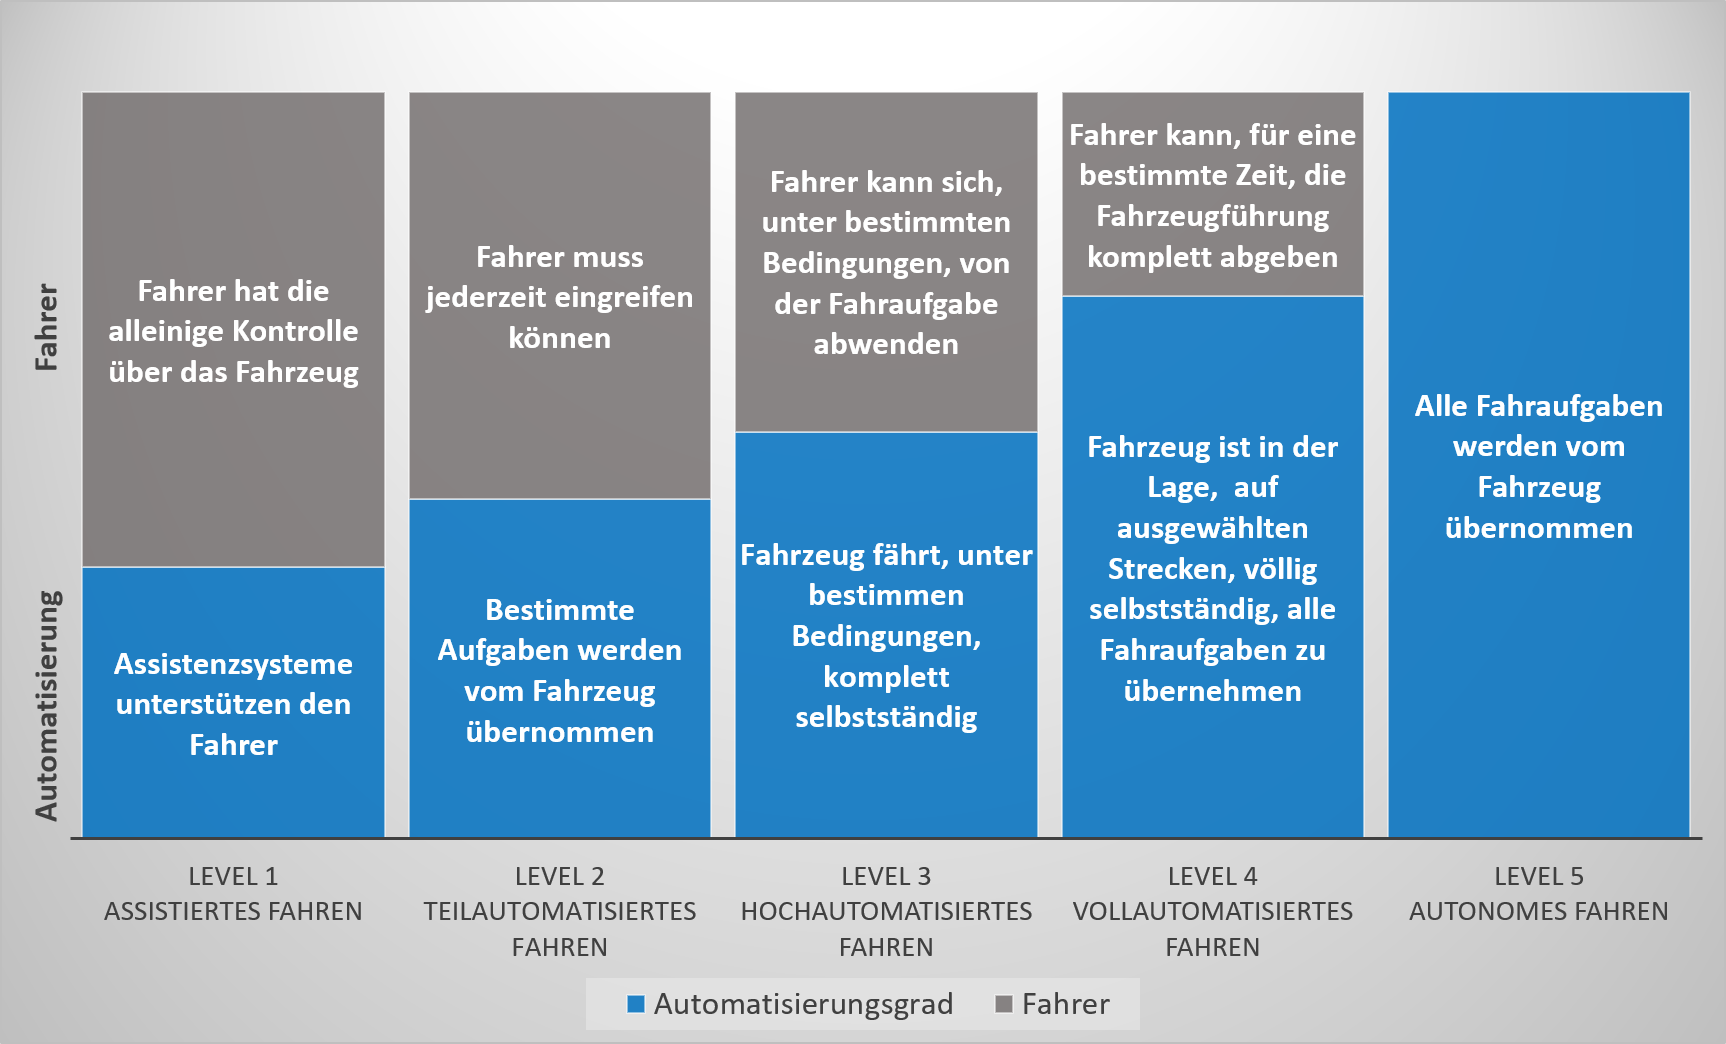
\includegraphics[width=\linewidth,height=0.6\linewidth]{fig/grundl/af/Level}
	\caption{Automatisierungsstufen des autonomen Fahrens}
	\label{img:grundl:af}
\end{figure}

Beim Level 1 des automatisierten Fahrens - oder auch assistiertem Fahren - hat der Fahrer durchgehend die alleinige Kontrolle �ber das Fahrzeug. Der Verkehr muss permanent im Blick behalten werden und die Haftung f�r Verkehrsverst��e oder Sch�den liegt beim Fahrer. Assistenzsysteme, wie der Abstandsregeltempomat, der je nach Abstand zum vorausfahrenden Fahrzeug bremst oder beschleunigt, unterst�tzen heute schon den Fahrer bei entsprechenden Fahraufgaben.
\\
\\
Bei Level 2-Fahrzeugen k�nnen, unter definierten Bedingungen, spezielle Aufgaben vom Fahrzeug selbst ausgef�hrt werden. So kann, ohne das Einwirken des Fahrers, beispielsweise auf der Autobahn die Spur gehalten, gebremst und beschleunigt werden. Dies wird, durch die Kombination von verschiedenen Assistenzsystemen, wie dem automatischen Abstandsregelautomat und dem Spurhalteassistent, m�glich. Im Vergleich zu Level 1, kann der Fahrer, w�hrend des teilautomatisierten Modus, die H�nde kurz vom Steuer nehmen. Dadurch werden Funktionen, wie der �berholassistent oder das automatische Einparken, erm�glicht. Dennoch muss der Fahrer, zu jeder Zeit, die Assistenzsysteme �berwachen und bei Fehlfunktionen eingreifen k�nnen, um das Fehlverhalten dann zu kompensieren. \\Schlie�lich liegt, im Falle eines Unfalls, die Verantwortung weiterhin bei ihm. 
\\
\\
Bei hochautomatisierten oder Level 3-Fahrzeugen darf sich der Fahrer, bei Hersteller-vorgege-benen Anwendungsf�llen, von der Fahraufgabe abwenden. Das Fahrzeug f�hrt, f�r diesen begrenzten Zeitraum, selbstst�ndig.
\\
\\
Beim vollautomatisiertem oder Level 4-Fahren kann der Fahrer die Fahrzeugf�hrung komplett abgeben. Bei Verkehrsverst��en, w�hrend der vollautomatisierten Fahrt, ist der Fahrer nicht haftbar. Das Fahrzeug ist in der Lage, auf bestimmten Strecken, v�llig selbstst�ndig, alle Fahraufgaben f�r eine l�ngere Zeit, zu �bernehmen. Die Insassen k�nnen w�hrenddessen, etwaigen Nebent�tigkeiten nachgehen. Das Fahrzeug kann allerdings auch ohne Insassen, entsprechende Fahraufgaben �bernehmen. So k�nnen Level 4-Fahrzeuge in Parkh�usern automatisiert einen Parkplatz suchen oder ebenso bei hohen Geschwindigkeiten auf die Autobahn auffahren, sich in den Verkehr einordnen und eigenst�ndig die Spur und den Abstand halten. Wenn das System w�hrend des vollautomatisierten Modus einen Fehler entdeckt, k�nnen die Passagiere entweder wieder die Kontrolle �bernehmen oder das Fahrzeug begibt sich in einen sicheren Zustand.
\\
\\
Das Level 5 oder autonome Fahren ist die letzte Stufe der Automatisierung bei Fahrzeugen. Es gibt keinen Fahrer mehr, sondern nur noch Passagiere, die nicht mehr f�r Verkehrsverst��e oder Sch�den haften. Die entsprechenden Hersteller, Halter oder Betreiber w�ren diesbez�glich haftbar beziehungsweise eine Versicherung m�sste f�r eventuelle Sch�den aufkommen.
\\
\\
Neben der Einstufung in 5 Level, gibt es noch ein Konzept mit drei Betriebsmodi. \\Der erste Betriebsmodus ist das unterst�tzende Fahren. In diesem muss der Fahrer den Verkehr stets im Blick behalten und ist alleine f�r die Fahrzeugf�hrung verantwortlich. Fahrassistenzsysteme unterst�tzen den Fahrer nur. Bei einem Fehlverhalten oder Versagen dieser, haftet der Fahrer f�r Verkehrsverst��e oder Unf�lle. Das automatisierte Fahren stellt den zweiten Betriebsmodus dar. Hierbei f�hrt das Fahrzeug, ausschlie�lich in vom Hersteller definierten Anwendungsf�llen, selbstst�ndig. Der Fahrer darf w�hrenddessen eine Nebent�tigkeit aus�ben. Bei Aufforderung des Systems, muss dieser aber kurzfristig die Kontrolle �bernehmen, da er sonst haftet. Im dritten Betriebsmodus, dem autonomen Fahren, f�hrt das Fahrzeug komplett selbstst�ndig. Das System beherrscht kritische Fahrsituationen. Bei etwaigen Betriebsst�rungen oder Fehlverhalten, muss ein Betreiber auf diese reagieren k�nnen. Dieser �berwacht das autonome Fahrzeug nur, ist allerdings nicht selber Fahrer. Die Passagiere haften in diesem Fall nicht.
\\
\\
Ein autonomes Fahrzeug muss seine Umgebung erfassen und die daraus gewonnen Informationen verarbeiten k�nnen. Hierzu werden verschiedenste Sensoren verwendet, die in \autoref{img:grundl:sensoren} dargestellt sind.
\begin{figure}
	\centering
	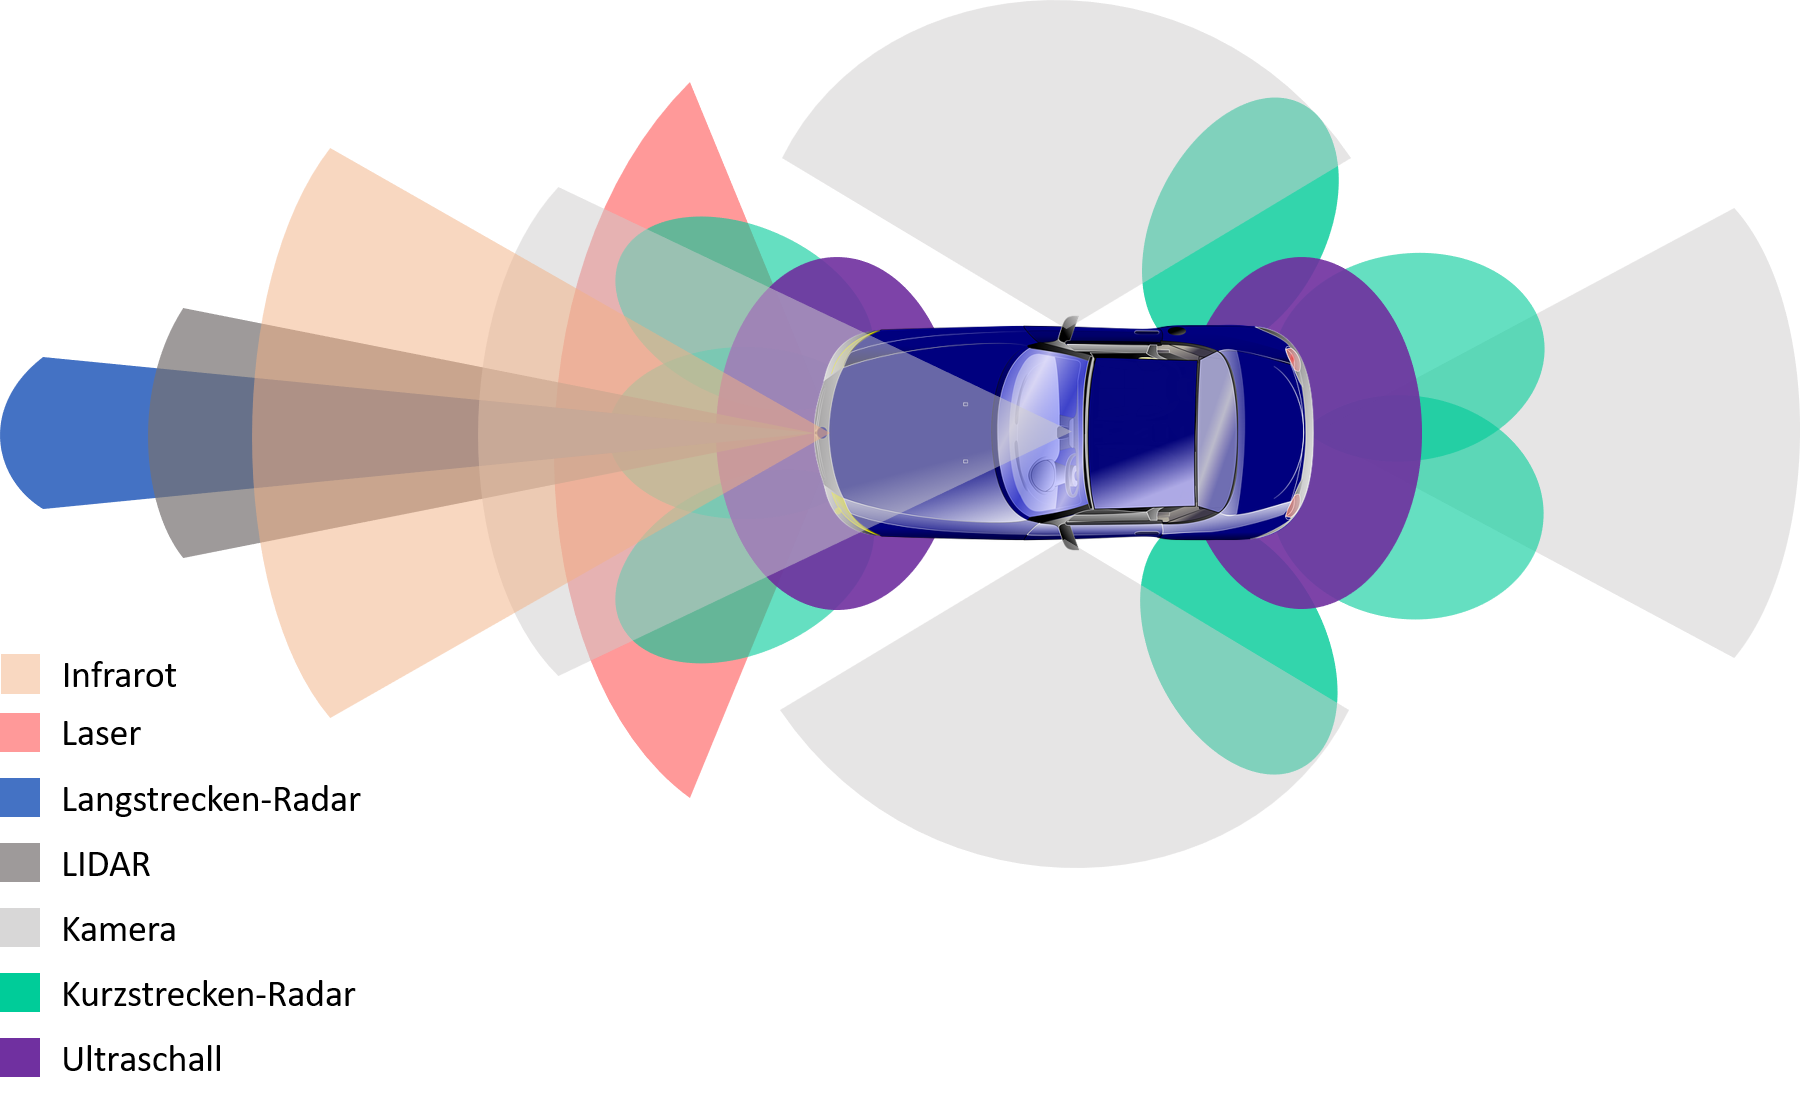
\includegraphics[width=0.9\linewidth,height=0.55\linewidth]{fig/grundl/af/Sensoren}
	\caption{Sensoren in einem Fahrzeug}
	\label{img:grundl:sensoren}
\end{figure}
Hierbei haben Ultraschallsensoren und Kurzstrecken-Radar eine kleine Reichweite und werden zur Hinderniserkennung sowie zum Parken eingesetzt. Langstrecken-Radar k�nnen Objekte in gro�er Entfernung sowie ihre Position und Geschwindigkeit bestimmen. LIDAR- und Laser-Sensoren erstellen, mit Hilfe von Laser-Licht, ein hochaufl�sendes 3D-Abbild der Umgebung. Zus�tzlich liefern Kamerasysteme, optische Informationen �ber Textur und Farbe eines Objektes. Infrarot-Sensoren sind vor allem f�r die Nachtsicht relevant. Durch die Kombination der verschiedenen Sensor-Daten ist eine nahezu exakte Erfassung des Umfelds m�glich. Diese Umgebungsdaten k�nnen, durch die Informationen von anderen Fahrzeugen sowie der Verkehrs-Infrastruktur, erg�nzt werden. Intelligente Softwarealgorithmen verarbeiten, mit Hilfe von leistungsstarken Microcontrollern und Prozessoren, die verschiedenen Daten, um das Fahrzeug autonom Fahren zu lassen. \cite{lit:af:sensoren}

\subsection*{\textbf{Motivation und Vorteile}}

Da bei autonomen Fahrzeugen kein Fahrer mehr notwendig ist, ergeben sich dadurch verschiedene Chancen und Vorteile in den Bereichen Gesellschaft, Wirtschaft und Sicherheit. Durch das Wegfallen eines Fahrers, haben die Passagiere, die gewonnene Fahrtzeit, f�r andere Aktivit�ten zur Verf�gung. Ebenso k�nnen durch das autonome Fahren Mobilit�tseingeschr�nkte, wie Personen im hohen Alter, mit Behinderungen oder ohne Fahrerlaubnis, durch eine erh�hte Mobilit�t verst�rkt am gesellschaftlichen Leben und Stra�enverkehr teilnehmen. \cite{lit:af:chancen}
\\
\\
Durch diese erh�hte Nutzer- und Kundengruppen, ergeben sich neue M�glichkeiten f�r Hersteller und Betreiber, diese durch neue Mobilit�tskonzepte, zu erschlie�en. Eines dieser Konzepte, n�mlich das Car-Sharing, gibt es bereits heute und kann auf das autonome Fahren angepasst werden. So k�nnte sich ein autonomes Fahrzeug selbstst�ndig, vom Nutzer aus, einen Parkplatz suchen und umgekehrt. Alternativ w�re es ebenso denkbar, dass sich das Fahrzeug eigenst�ndig zum gew�nschten Zielort des n�chsten Nutzers bewegt. \cite{lit:af:chancen}
\\
\\
Hinzu kommen, durch das Wegfallen des Fahrers, bei autonomen �ffentlichen Verkehrsmitteln, eine h�here Flexibilisierung und Bedarfsorientierung in Bezug auf Einsatzzeit und -gebiet. Durch eine hohe Anzahl an Sensoren, die verschiedene Daten erfassen, ergibt sich eine gro�e Menge an Informationen, wodurch autonome Fahrzeuge pr�ziser durch den Stra�enverkehr man�vrieren k�nnen. Dadurch ergibt sich eine Reduzierung der ben�tigten Verkehrs- und Parkfl�chen, insbesondere in Stadtzentren. \cite{lit:af:chancen}
\\
\\
Ebenso werden die Kapazit�ten im Stra�enverkehr effizienter genutzt, da die ben�tigte Zeit, beispielsweise beim Abbiegevorgang, an Lichtanlagen sowie die Reaktionszeit verringert werden kann. Es werden, im Allgemeinen, h�here Geschwindigkeiten im Stra�enverkehr erm�glicht. Aufgrund dieser Aspekte, ergeben sich entsprechende Rationalisierungseffekte. Das Wegfallen eines Fahrers f�hrt beispielsweise im Mobilit�ts- und Transportsektor zu Kosteneinsparungen und somit zu Effizienzsteigerungen. Dadurch werden ebenso die Umweltauswirkungen im Stra�enverkehr verringert, da Fahrvorg�nge optimiert werden und somit der Energie- und Emissionsaussto� sinkt. \cite{lit:af:chancen}
\\
\\
In Deutschland waren in 2017 91\% der Verkehrsunf�lle auf menschliches Versagen zur�ckzuf�hren \cite{lit:af:unfall}. Dies entsprach der Hauptunfallursache im Stra�enverkehr. Bei autonomen Fahrzeugen kann diese als Unfallursache ausgeschlossen werden, welches zu einer Erh�hung der Verkehrssicherheit f�hrt. Hierf�r m�ssen allerdings autonome Fahrzeuge komplexe Verkehrssituationen und fahrkritische Szenarien wahrnehmen und interpretieren k�nnen.

\subsection*{\textbf{Blick in die Zukunft}}

Derzeit befinden sich auf den deutschen Stra�en h�chstens Level 2-Fahrzeuge. Diese sind mit Assistenzsystemen ausger�stet, welche es dem Fahrer erlauben, kurzfristig die Kontrolle �ber die Lenkung abzugeben. Laut einer Studie von deloitte m�chten aktuell 90\% der befragten Fahrer aber ebenso jederzeit die Kontrolle �ber ihr Fahrzeug �bernehmen k�nnen \cite{lit:af:deloitte}. Das zeigt auf, dass die Akzeptanz und das Vertrauen in autonome Fahrzeuge noch stark verbessert werden muss, bevor sich diese im deutschen Stra�enverkehr durchsetzen k�nnen. \\Die Sicherheit und Verl�sslichkeit des Systems sind hierbei die kritischen Faktoren. 
\\
\\
Demgegen�ber stehen Aspekte, wie der erh�hte Komfort und die Erschlie�ung neuer Mobilit�tskonzepte. Durch autonome Fahrzeuge k�nnen Flottenbetreiber individuellere Mobilit�ten erm�glichen, wodurch sich ebenso der Trend vom Besitz zum Car-Sharing verst�rken k�nnte. Viele weitere Faktoren und Rahmenbedingungen m�ssen jedoch erst noch gekl�rt werden, damit sich die Akzeptanz f�r das autonome Fahren erh�ht und dieses realisierbar wird. Durch diese Herausforderungen ist eine Einf�hrung von Level 4- oder Level 5-Fahrzeugen, voraussichtlich, nicht vor 2040 zu erwarten. \cite{lit:af:prognose}


\subsection*{\textbf{Herausforderungen}}

Bevor sich autonome Fahrzeuge im Stra�enverkehr durchsetzen, gibt es einige Herausforderungen, die vorher zu bew�ltigen sind. Die Wichtigste stellt hierbei das System f�r autonome Fahrzeuge an sich dar. Diese m�ssen im dynamischen Stra�enverkehr mit jeder Situation umgehen k�nnen. Dazu muss die gesamte Umgebung in Echtzeit erfasst und die Fahrsituation interpretiert werden. Die gesammelten Daten dienen als Grundlage f�r die Bestimmung der eigenen Fahrzeugbewegung sowie f�r Prognosen �ber die Bewegung der weiteren Verkehrsteilnehmer. Diese Anforderungen muss das System, ebenso in komplexen Situationen, regelkonform bew�ltigen, um die Sicherheit der Insassen und anderer Verkehrsteilnehmer zu gew�hrleisten. \cite{lit:af:chancen}
\\
\\
Zus�tzlich muss dieses Systemfehler erkennen und sich bei Bedarf in einen sicheren Zustand begeben k�nnen. Um so ein System zu gew�hrleisten, werden mehr Informationen als bei konventionellen Fahrzeugen, ben�tigt. Hierzu muss die entsprechende Infrastruktur noch entwickelt bzw. ausgebaut werden, damit die schnelle und fehlerfreie Fahrzeugkommunikation, unter Fahrzeugen, sichergestellt werden kann. Die erh�hte Anzahl an Kommunikationsschnittstellen stellen allerdings auch steigende Angriffsvektoren dar. Personenbezogene Daten wie die Adresse, Fahrtziele oder audiovisuelle Aufzeichnungen m�ssen sicher und anonymisiert gespeichert werden. Au�erdem w�chst das Risiko von Cyberangriffen auf die digitale Infrastruktur und autonome Fahrzeuge. Dies z�hlt zum Bereich Security. \cite{lit:af:cyber}
\\
\\
Der langsame Wandel des Stra�enverkehrs und der Infrastruktur wird die Einf�hrung des Mischverkehrs, von konventionellen und autonomen Fahrzeugen, unvermeidbar machen, wodurch viele ethische Fragen im Bezug auf die Haftung gekl�rt werden m�ssen. Ein zentrales Problem bei autonomen Fahrzeugen, ist das ethisch korrekte Verhalten im Stra�enverkehr. Eine hohe Anzahl an Faktoren nehmen auf die Algorithmen autonomer Fahrzeuge Einfluss, wodurch Dilemma-Situationen entstehen k�nnen. Eine solche Situation kann auftreten, wenn \zB eine Person eine rote Ampel �berquert. Ein autonomes Fahrzeug, dass durch eine Notbremsung nicht mehr vor dem Fu�g�nger zum Halten kommen kann, wird hier versuchen, ein Ausweichman�ver durchzuf�hren. Wenn sich auf der Gegenfahrbahn Fahrzeuge mit weiteren Insassen befinden, bleibt noch die Option auf den Gehweg auszuweichen. Angenommen, dass sich auf diesem auch Personen befinden, kann das autonome Fahrzeug einen Personenschaden nicht verhindern. Wer in solchen F�llen haftet und wie in diesen und weiteren fahrkritischen Szenarien entschieden werden soll, ist ein Kernaspekt, der noch zu kl�ren ist. Um die Akzeptanz f�r das autonome Fahren, als Technologie bzw. Mobilit�tskonzept, zu st�rken, ist es essentiell, diese Herausforderungen zu l�sen. \cite{lit:af:ethik}

\FloatBarrier
\section{K�nstliche Intelligenz und Maschinelles Lernen}
\label{sec:grundl:ki}

Der Begriff k�nstliche Intelligenz wird in verschiedenen Anwendungsbereichen genannt. Dieser ist allerdings sehr abstrakt. F�r die allgemeine Bev�lkerung ist es unklar, welches Problem gel�st werden soll und welche L�sungsalgorithmen eingesetzt werden. Der Grund hierf�r liegt zum Teil in der Komplexit�t dieser Algorithmen. Im Folgenden wird diese Thematik n�her betrachtet und erl�utert.

\subsection*{\textbf{Definition von k�nstlicher Intelligenz}}
Die Informatik enth�lt viele Teilgebiete. Der Bereich Data Science z�hlt dazu. Dieses Gebiet befasst sich damit, Erkenntnisse aus gro�en Datens�tzen, zu gewinnen. Hierzu werden meist statistische Methoden angewandt. Ein spezieller Bereich dieses Themenbereichs ist die k�nstliche Intelligenz. Hierbei wird das kognitive Verhalten des Menschen imitiert. Ein spezieller Fall von k�nstlicher Intelligenz ist das Machine Learning. Dabei wird, anders als in anderen Teilgebieten der Informatik, kein L�sungsalgorithmus vorgegeben. Die Algorithmen erkennen, durch wiederholtes Ausf�hren, selbstst�ndig Strukturen und Muster in den Daten und k�nnen so spezielle Aufgaben l�sen. Das maschinelle Lernen kann in drei Arten eingeteilt werden. Dazu z�hlen das �berwachte (supervised), unbewachte (unsupervised) und best�rkende (reinforcement) Lernen. \cite{lit:ki:def}

\begin{figure}
	\centering
	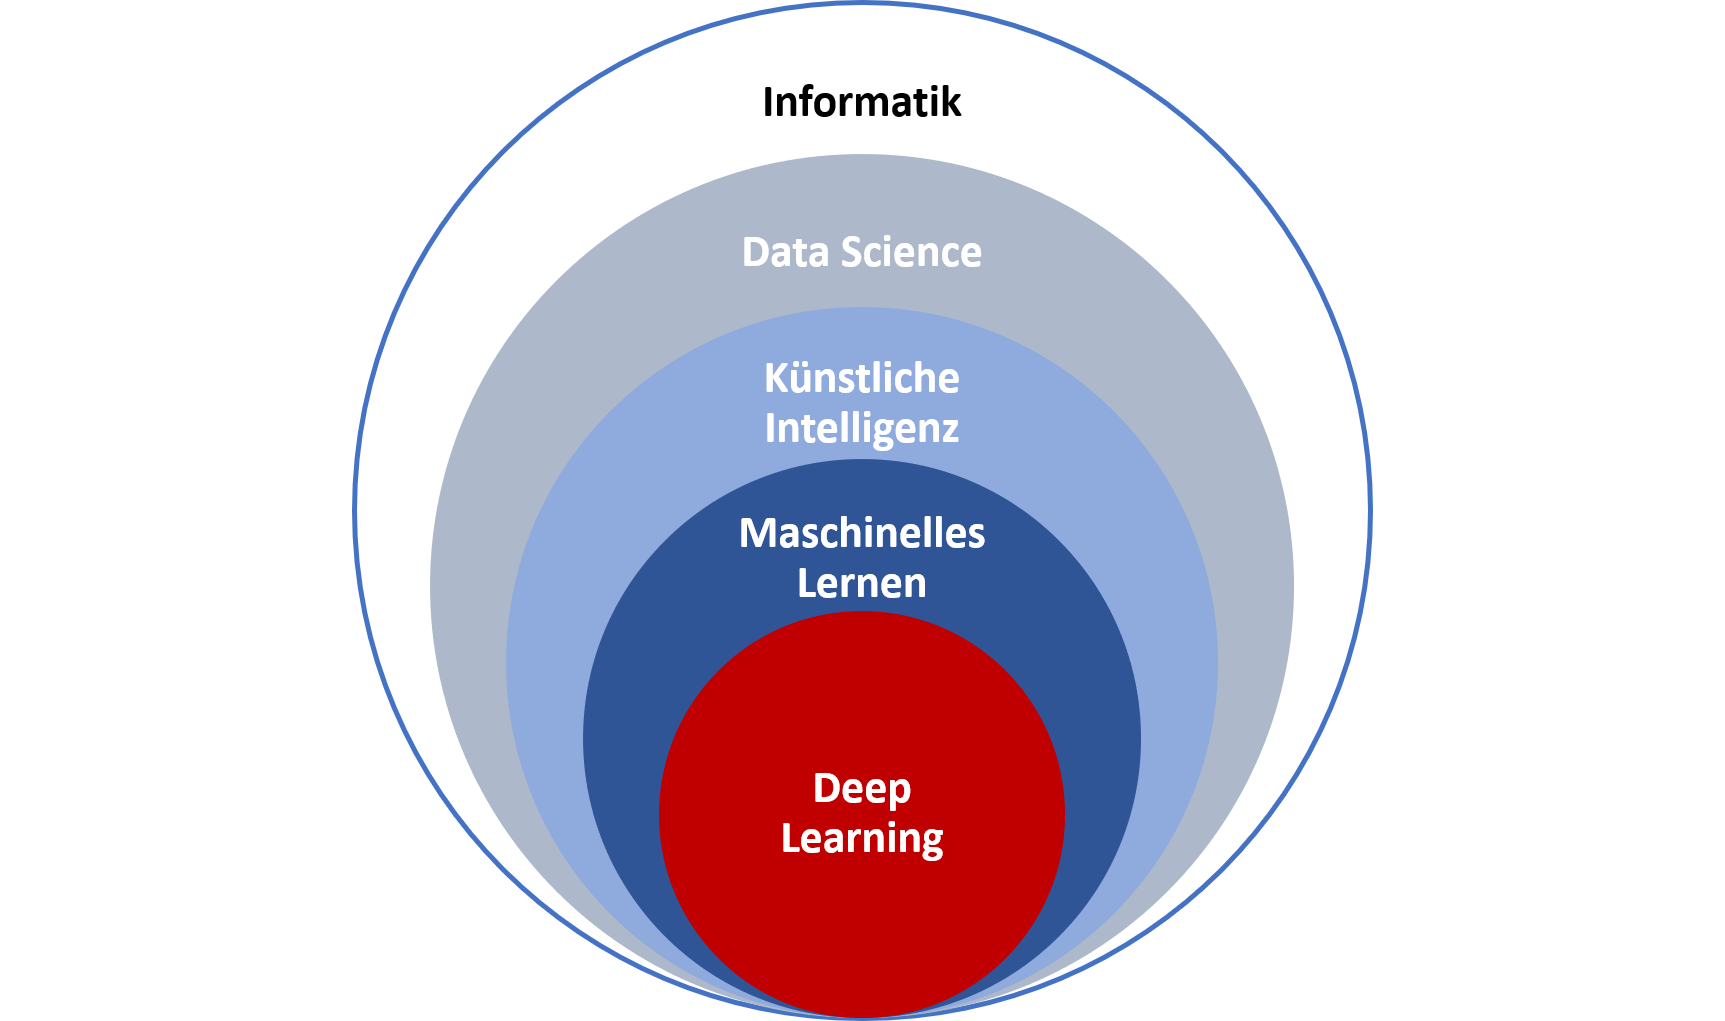
\includegraphics[height=0.6\linewidth,width=\linewidth]{fig/grundl/ki/KI}
	\caption{Teilgebiete der Informatik}
	\label{img:grundl:ki}
\end{figure}

\subsection*{\textbf{Supervised Learning}}
Das Supervised Learning zeichnet sich dadurch aus, dass bereits ein kategorisierter Datensatz vorliegt und so Machine Learning-Algorithmen direktes Feedback erhalten. Es besteht grunds�tzlich die Aufgabe, einen gewissen Output zu prognostizieren. Wenn der Input einer bestimmten Klasse zugeh�rig ist, welche bestimmt werden soll, handelt es sich um eine Klassifizierung. Der Begriff �berwachtes Lernen kommt daher, dass die Trainingsdatens�tze, mit dem das Modell trainiert wird, bereits Labels enthalten, also in Klassen kategorisiert sind. Ein Beispiel f�r solche Labels k�nnen beispielsweise Buchstaben oder Ziffern sein. Das Modell kann allerdings nur diejenigen Labels bestimmen, die ebenso im Trainingsdatensatz vorhanden sind. Eine sogenannte Regressions-Aufgabe ist gegeben, falls die Ausgabe eines Machine Learning-Modells, die Prognose eines kontinuierlichen Wertes entspricht. Durch diese kontinuierlichen Modelle, lassen sich beispielsweise Vorhersagen �ber die Zukunft treffen. In beiden F�llen ist das Ziel, ein Modell zu erlernen, welches Prognosen �ber neue Daten bereitstellt. \cite{lit:Raschka2019}

\subsection*{\textbf{Unsupervised Learning}}

Im Gegensatz zum Supervised Learning, steht beim Unsupervised Learning kein Datensatz, mit bereits bekannten Labels, zur Verf�gung. \\Diese Modelle und Algorithmen finden eigenst�ndig Muster in Datens�tzen und deren Eigenschaften. Eine Kategorie des Unsupervised Learning ist die Cluster-Analyse. Ziel dieser ist es, versteckte Strukturen in Datens�tzen zu finden oder diese passend in Clustern zu gruppieren. Ein weiterer Anwendungsfall f�r das Unsupervised Learning, ist die Sprachverarbeitung oder auch Natural Language Processing. Hierbei wird die Sprache, in ihren verschiedenen Formen, analysiert. Die Sentimentanalyse, also die Analyse der menschlichen Stimmung und das Nutzerverhalten, ist ein Teilgebiet dieser Sprachverarbeitung. Generative Algorithmen geh�ren ebenso zum Bereich des Unsupervised Learning. Auf diesen Algorithmentyp wird sp�ter n�her eingegangen. \cite{lit:Raschka2019}

\subsection*{\textbf{ReinforcementLearning}}
Eine weitere Art des maschinellen Lernens ist das Reinforcement Learning. Hierbei werden sogenannte Agenten analysiert, die durch Belohnungen oder Bestrafungen ihr Ziel, in einer bestimmten Umgebung oder Aufgabenstellung, optimieren. \cite{lit:Raschka2019}

\subsection*{\textbf{Neuronale Netze}}

Ein bekanntes Beispiel f�r ein Machine Learning-Modell bilden neuronale Netze (\textit{engl.: Neural Networks}). Diese sind inspiriert durch den Aufbau der Nervenzellen im menschlichen Gehirn. Wie im menschlichen Gehirn, werden hier k�nstliche Neuronen bzw. Synapsen, in Form von Reihen aus Datenknoten, miteinander verbunden. Weiterhin werden diese Verbindungen gewichtet. Bei jedem Lerndurchlauf der Daten werden diese Gewichte angepasst, bis das Modell zufriedenstellend arbeitet. Sobald das neuronale Netz, durch den Lernvorgang, die einzelnen Gewichte gelernt hat, kann es ebenso auf neue Daten angewandt werden. \newpage Falls das Netz versteckte Schichten enth�lt, die nicht direkt mit einer Ein- oder Ausgabeschicht verbunden sind, so handelt es sich um ein tiefes neuronales Netz (\textit{engl.: Deep Neural Network}). Umso mehr Schichten ein Deep Neural Network aufweist, desto komplexere Muster kann es erkennen bzw. erlernen, sowie anspruchsvollere Aufgaben l�sen. \cite{lit:Raschka2019}
%\workTodo{latex tikz package neuronales netz bild erstellen}
%\begin{figure}
%	\centering
%	\begin{tikzpicture}[shorten >=1pt,->,draw=black!50, node distance=\layersep]
%		\tikzstyle{every pin edge}=[<-,shorten <=1pt]
%		\tikzstyle{neuron}=[circle,fill=black!25,minimum size=17pt,inner sep=0pt]
%		\tikzstyle{input neuron}=[neuron, fill=green!50];
%		\tikzstyle{output neuron}=[neuron, fill=red!50];
%		\tikzstyle{hidden neuron}=[neuron, fill=blue!50];
%		\tikzstyle{annot} = [text width=4em, text centered]
%		
%		% Draw the input layer nodes
%		\foreach \name / \y in {1,...,4}
%		% This is the same as writing \foreach \name / \y in {1/1,2/2,3/3,4/4}
%		\node[input neuron, pin=left:Input \#\y] (I-\name) at (0,-\y) {};
%		
%		% Draw the hidden layer nodes
%		\foreach \name / \y in {1,...,5}
%		\path[yshift=0.5cm]
%		node[hidden neuron] (H-\name) at (\layersep,-\y cm) {};
%		
%		% Draw the output layer node
%		\node[output neuron,pin={[pin edge={->}]right:Output}, right of=H-3] (O) {};
%		
%		% Connect every node in the input layer with every node in the
%		% hidden layer.
%		\foreach \source in {1,...,4}
%		\foreach \dest in {1,...,5}
%		\path (I-\source) edge (H-\dest);
%		
%		% Connect every node in the hidden layer with the output layer
%		\foreach \source in {1,...,5}
%		\path (H-\source) edge (O);
%		
%		% Annotate the layers
%		\node[annot,above of=H-1, node distance=1cm] (hl) {Hidden layer};
%		\node[annot,left of=hl] {Input layer};
%		\node[annot,right of=hl] {Output layer};
%	\end{tikzpicture}
%\end{figure}

\subsection*{\textbf{Anwendungen}}

Im Bereich der k�nstlichen Intelligenz hat es, in den letzten Jahren, enorme Fortschritte gegeben. Dadurch wurden neue M�glichkeiten und Anwendungsgebiete erschlossen. Mithilfe von Machine Vision-Algorithmen k�nnen Bilder analysiert und kategorisiert werden. Die extrahierten Informationen bilden die Basis f�r weitere Analysen. Hierf�r finden sich beispielsweise Einsatzgebiete in der medizinischen Diagnostik, sowie bei der Erkennung von Personen und Gesichtern. Ein weiteres Einsatzgebiet, f�r das maschinelle Lernen, ist die Mustererkennung. Gro�e Datenmengen oder -str�me sind f�r den Menschen schwer zu interpretieren, wohingegen Machine Learning-Algorithmen leichter diese Muster erkennen und dem Menschen Erkenntnisse liefern k�nnen. Mithilfe von k�nstlicher Intelligenz und den einzelnen Teildisziplinen lassen sich einige, der in \autoref{sec:grundl:af} genannten Herausforderungen und Anforderungen, l�sen. Durch die Bilderkennung lassen sich beispielsweise Personen und Fahrzeuge im Stra�enverkehr von autonomen Fahrzeugen identifizieren, wodurch diese ihre entsprechende Fahrtrajektorie planen k�nnen. Damit kann die Sicherheit, aller am Stra�enverkehr Beteiligten, sichergestellt werden. \cite{lit:ki:anw}

\FloatBarrier
\section{Generative Algorithmen}
\label{sec:grundl:gan}

Die Modelle der k�nstlichen Intelligenz, die in \autoref{sec:grundl:ki} unter Supervised Learning genannt wurden, werden als diskriminative Algorithmen bezeichnet. So lassen sich, bei neuem Input, Prognosen dar�ber machen, zu welcher Klasse dieser wahrscheinlich geh�rt. Anders ausgedr�ckt, wird also die Wahrscheinlichkeit $p(y|x)$ gesch�tzt, dass ein Input $x$ der Klasse $y$ zugeh�rig ist. In den letzten Jahrzehnten wurden vorwiegend in den Bereichen von diskriminativen Algorithmen, speziell in der Klassifizierung, Fortschritte erzielt. 
\\
\\
In diesem Kapitel sollen nun generative Algorithmen n�her betrachtet werden. Erst in den letzten 5 bis 10 Jahren ergab sich eine st�rkere Pr�senz der generativen Algorithmen in der Praxis. Als wesentliche Grundlage diente hierbei die Funktionsweise eines sogenannten Autoencoders. Hierbei erm�glicht ein Encoder, hochdimensionale Merkmalsvektoren in einen niederdimensionalen latenten Raum, zu komprimieren. Basierend auf dem latenten Raum kann ein Decoder, mithilfe einer Transformation, den Originaldatensatz r�ckgewinnen. Ein solcher latenter Raum erzielt ebenso eine h�here Transparenz der wesentlichen Daten. Durch die Verwendung einer Verteilungsfunktion �ber diesem latenten Raum, erh�lt der Output eine Varianz, ist aber trotzdem �hnlich wie der Input. Bei der generativen  Modellierung sind normalerweise ungelabelte Datens�tze die Basis f�r die Algorithmen. Es handelt sich also um eine Form des Unsupervised Learning. Hierbei wird $p(x)$, also die Wahrscheinlichkeit $x$ zu beobachten, gesch�tzt. Allerdings gibt es ebenso generative Modelle, die eine Mischform aus Supervised und Unsupervised Learning darstellen, falls ein gelabelter Datensatz vorliegt. In diesem Fall wird die Verteilung $p(x|y)$ gesch�tzt, also die Wahrscheinlichkeit $x$, bei gegebenen Labels $y$, zu beobachten. Bei generativen Algorithmen ist demnach die zugrundeliegende Verteilung des Datensatzes von Interesse. \cite{lit:Foster2020}
\\
\\
Durch den Fokus auf eine derartige Verteilung der Daten ist es m�glich, neue synthetische Daten zu generieren. Dabei ist davon auszugehen, dass ein Datensatz einer bestimmten Verteilung $p_{data}$ zugrunde liegt. Mit einem generativen Modell wird versucht, diese mit einer neuen Verteilung $p_{model}$ nachzubilden oder abzusch�tzen. Dieser Vorgang gilt als erfolgreich, sofern durch $p_{model}$ Daten generiert werden k�nnen, die �hnlich wie die zugrundeliegenden Daten sind, sich allerdings so weit davon unterscheiden, dass sie nicht nur Reproduktionen oder aufgepr�gtes Rauschen abbilden.\cite{lit:Foster2020}

\subsection*{\textbf{Taxonomie von generativen Algorithmen}}

Die grundlegenden generativen Algorithmentypen lassen sich, im Rahmen einer allgemeing�ltigen Taxonomie, gruppieren. Eine derartige Taxonomie ist in \autoref{img:grundl:gan} dargestellt \cite{lit:Goodfellow2017}.

\begin{figure}
	\centering
	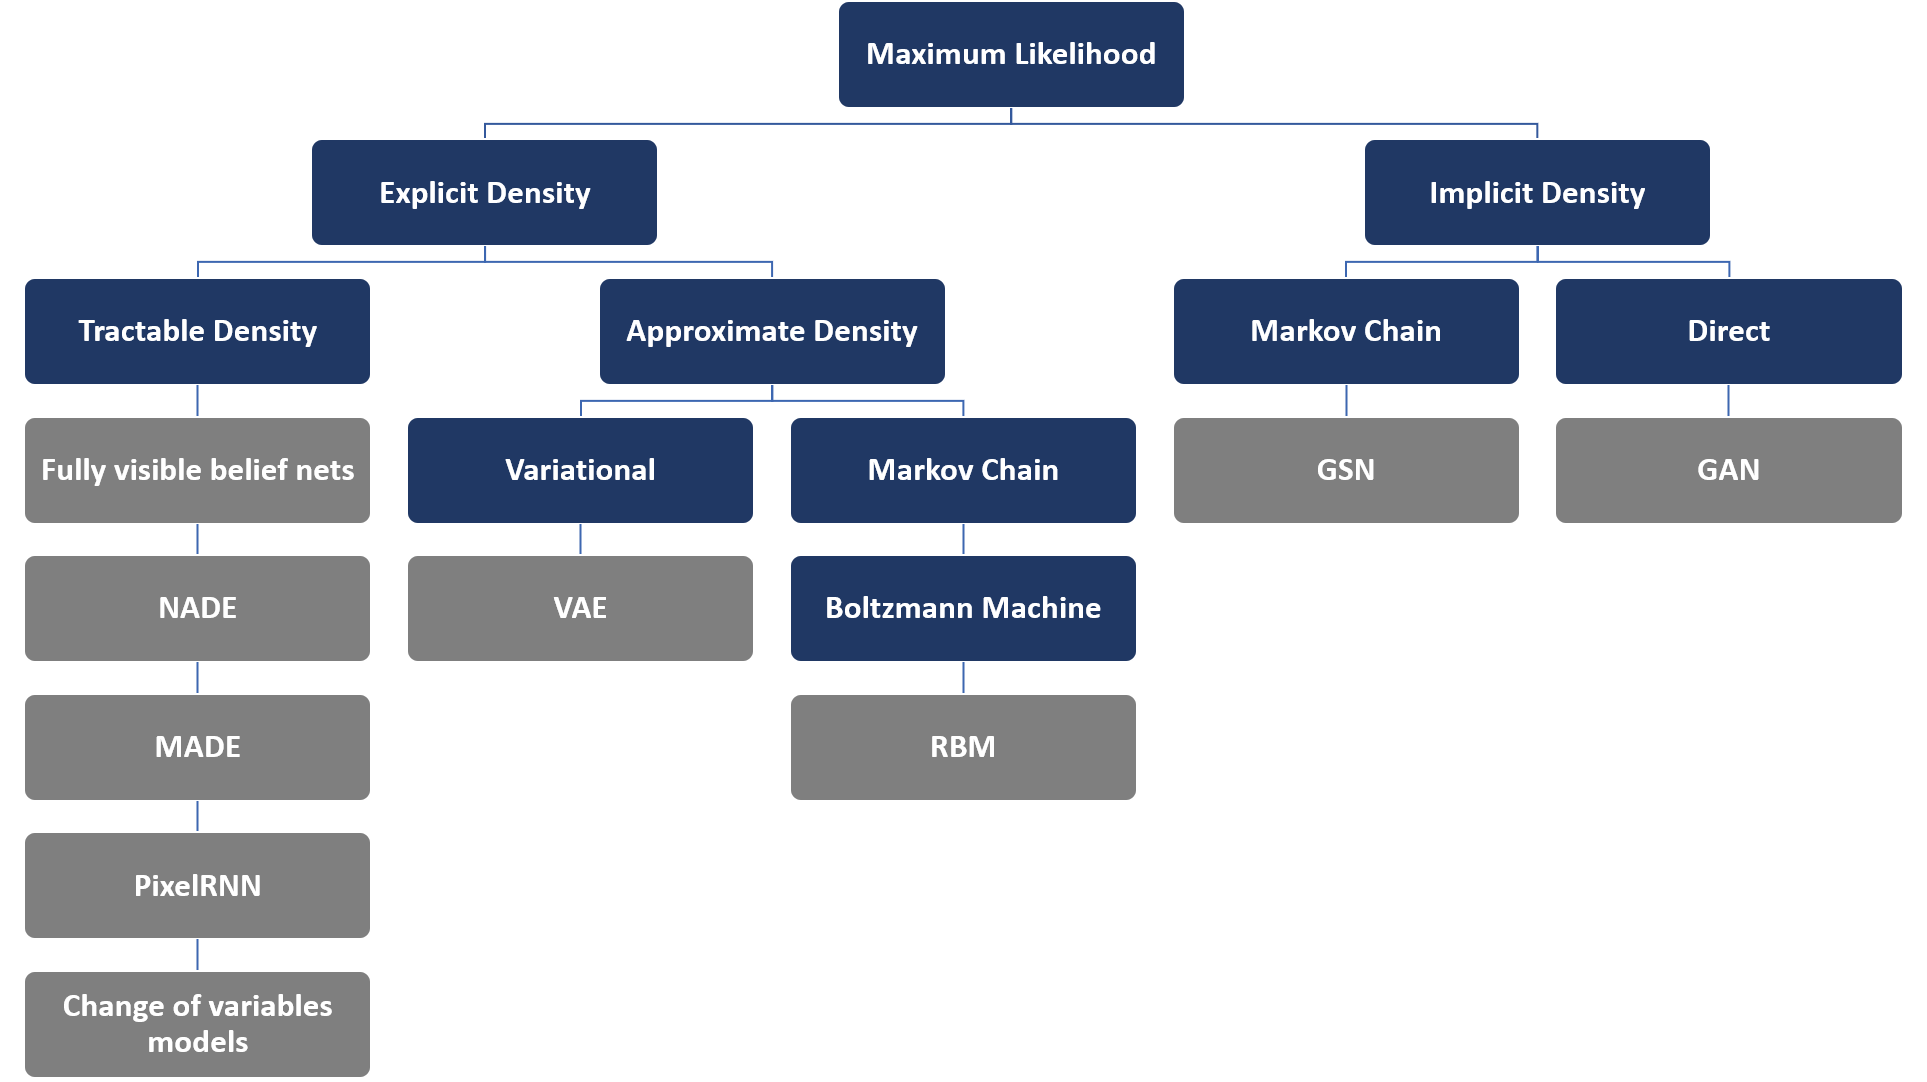
\includegraphics[width=\linewidth,height=0.6\linewidth]{fig/grundl/gan/GAN}
	\caption{Grundlegende Taxonomie von generativen Algorithmen}
	\label{img:grundl:gan}
\end{figure}

Hierbei werden alle Algorithmen von der Maximum Likelihood Estimation abgeleitet. Eine erste Gruppierung erfolgt in Bezug auf die Wahrscheinlichkeitsdichtefunktion der zugrundeliegenden Datenmenge. Zum einen kann diese explizit bzw. als geschlossener Ausdruck angegeben sein. Zum anderen kann diese implizit bzw. w�hrend des Trainingsvorgangs, gesch�tzt werden.
\\
\\
Die expliziten Modelle k�nnen weiter in die Tractable Density und die Approximate Density unterteilt werden. Die Tractable Density Modelle k�nnen hierbei in Polynomialzeit berechnet werden. \newpage Zu diesen geh�ren generative Algorithmen wie die Fully visible belief nets, Neural Autoregressive Distribution Estimation (NADE), Masked Autoencoder for Distribution Estimation (MADE), Pixel Recurrent Neural Networks (PixelRNN) oder Change of variable models. Die Approximate Modelle sch�tzen, w�hrend des Trainingsvorgangs, eine explizite Dichtefunktion. Diese Approximation erfolgt entweder deterministisch oder stochastisch. Zu diesen Modellen geh�ren beispielsweise die Variational Autoencoder (VAE) oder Restricted Boltzmann Machines (RBM).
\\
\\
Die impliziten generativen Modelle approximieren die Dichtefunktion eines Trainingsdatensatzes. Zu diesen geh�ren, die auf Markov-Ketten basierenden Generative Stochastic Networks (GSN) sowie die sogenannten Generative Adversarial Networks (GAN). Letztere erlangten, in den letzten Jahren, eine gro�e Popularit�t und werden, im Folgenden, n�her beschrieben.

\subsection*{\textbf{Generative Adversarial Networks}}

Das Generative Adversarial Network ist ein generatives Modell, mit dem es m�glich ist, synthetische Daten zu erzeugen. Dieser Algorithmus enth�lt, wie typische generative Algorithmen, einen Generator, der eine, auf dem Trainingsdatensatz basierende, Verteilung generiert. Neben dem generativem Anteil umfasst es jedoch noch ein diskriminatives Modell. Dieser Diskriminator lernt zu bestimmen, ob Daten aus dem generativen Modell stammen oder reale Daten vorliegen. W�hrend des Lernvorgangs generiert der Generator synthetische Daten, die mit der Zeit immer mehr der Verteilung des zugrundeliegenden Trainingsdatensatzes entsprechen. Der Diskriminator versucht dann, diese korrekt, in reale oder generierte Samples einzuteilen. \cite{lit:Raschka2019}
\\
\\
Zu Beginn des Trainingsvorgangs wird der Generator mit einem Zufallsvektor $z$ initialisiert. Danach werden abwechselnd der Diskriminator und der Generator trainiert bzw. optimiert. Dabei werden die Parameter der einen Komponente stets festgehalten, solange die jeweils andere trainiert wird. Der Diskriminator versucht, die Wahrscheinlichkeit zu maximieren. Der Generator hingegen verfolgt das Ziel, dessen Verlustfunktion zu minimieren. Diese wird wie folgt beschrieben \cite{lit:Goodfellow2014}:

\begin{equation}
	\min\limits_{G} \, \max\limits_{D} \, V(D,G) = E_{x \sim p_{Data}(x)} \left[\log D(\mathbf{x})\right] + E_{x \sim p_{x}(x)} \left[\log(1 -  D(G(z)))\right]
	\label{eqn:gan:loss}
\end{equation}

Der Ausdruck $E_{x \sim p_{Data}(x)}\left[\log D(\mathbf{x})\right]$ stellt den Erwartungswert in Bezug auf die Verteilung des Realdatensatzes dar. $E_{x \sim p_{x}(x)} \left[\log(1 -  D(G(z)))\right]$ bezeichnet hierbei den Erwartungswert, bezogen auf die Verteilung des Inputvektors $z$. \cite{lit:Raschka2019}

\FloatBarrier
\section{Zeitreihen}
\label{sec:grundl:time}

Sequenzielle Daten stellen eine geordnete Liste von Ereignissen dar. Diese Art von Daten findet sich in verschiedenen Anwendungsf�llen wieder. So kommen in der Biologie oftmals sequenzielle Daten, \zB in der DNA oder in Proteinsequenzen, vor. Auch symbolische Sequenzen, wie die logische Folge eines Kundenkaufs in einem Onlineshop, fallen unter diese Kategorie. Eine weitere wichtige Art von sequenziellen Daten sind Zeitreihen.
\\
\\
Dabei handelt es sich um numerische Daten, zwischen denen, normalerweise, ein festes diskretes Zeitintervall liegt. Zeitreihen finden sich in verschiedensten Anwendungsgebieten. Diese kommen in der Natur, in Form von Temperatur oder Klima, sowie in der Wirtschaft, in Form von Aktienkursen, vor. Die in Fahrzeugen gespeicherten Sensordaten bilden ebenfalls Zeitreihen. Mithilfe der Zeitreihenanalyse l�sst sich die Struktur der Zeitreihen verstehen. Es lassen sich Anwendungen in den verschiedenen Bereichen simulieren und vergleichen, sowie Prognosen erstellen. \cite{lit:Kreiss2006}
\\

\subsection*{\textbf{Taxonomie von Zeitreihen}}

Es gibt verschiedene Arten von Zeitreihen, die sich anhand bestimmter Faktoren, unterscheiden. Im Folgenden werden die wesentlichen Typen von Zeitreihen, auf Basis von \cite{lit:time:tax}, n�her beschrieben.

\begin{center}
	\begin{longtable}[h!]{p{0.5\linewidth}|p{0.5\linewidth}}
		%\centering
		%\begin{tabular}{p{0.4\linewidth}|p{0.4\linewidth}}
			\toprule
			\textbf{Arten von Zeitreihen} & \textbf{Beschreibung} \\ 
			\midrule
			Kontinuierlich und Diskret & Die zugrundeliegenden Daten k�nnen von kontinuierlicher Natur sein, wie \zB physikalische Daten, wie die Temperatur. In diesem Fall handelt es sich um kontinuierliche Zeitreihen $x(t)$. Bei diskreten Datenpunkten, die nach bestimmten Intervallen abgerufen werden, \zB jede Sekunde, handelt es sich um diskrete Zeitreihen $x_{t_{i}}$. Kontinuierliche Zeitreihen k�nnen durch Abtastung in diskrete umgewandelt werden. \\
			\midrule
			Gleichm��ig und Ungleichm��ig Abgetastet &  Bei diskreten Zeitreihen werden die Daten in bestimmten Intervallen erhoben. Wenn dieses Intervall zwischem jeden Datenpunkt gleich ist, so handelt es sich um einen gleichm��ig abgetasteten Datensatz. Bei einem ungleichm��ig abgetasteten Datensatz ist dieses Abtastintervall nicht f�r alle Zeitpunkte konstant.\\
			\midrule
			Univariat und Multivariat & Eine univariate Zeitreihe $x(t)$ oder $x_t$, ist durch eine, nach der Zeit, geordnete endliche Sequenz von $T$ Datenpunkten definiert. F�r jeden Zeitpunkt $t_i$ gibt es genau einen Datenpunkt $x_{t_i}$. Eine multivariate Zeitreihe besteht aus $M > 1$ univariaten Zeitreihen. F�r jeden Zeitpunkt $t_i$ gibt es also $M$ Datenpunkte $x_{u,t_i}$. Folgend wird also bei univariaten Zeitreihen nur ein Merkmal und bei multivariaten mehrere betrachtet. \\
			\midrule
			Periodisch und Aperiodisch & Wenn kein periodisches Verhalten festgestellt werden kann, wird diese als aperiodisch bezeichnet. Falls Datenpunkte periodisches Verhalten aufweisen, handelt es sich um periodische Zeitreihen. Bei vollst�ndig periodischen Zeitreihen zeigen alle Datenpunkte periodisches Verhalten auf. Tritt nur in einer Teilmenge von Datenpunkten periodisches Verhalten auf, wird diese als partiell-periodische Zeitreihe bezeichnet. Ein weiterer Faktor ist die Synchronizit�t der periodischen Muster. Synchrone Muster treten mit einer fixen Periode auf, wohingegen asynchrone Muster keine feste Periode aufweisen. \\ %Ein weiterer Aspekt der bei der Zeitreihenanalyse betrachtet werden sollte ist die Periodizit�t der univariaten Zeitreihen. Hier wird die Zeitreihe auf periodisches Verhalten untersucht und in welcher Form dieses auftaucht. 
			\midrule
			Station�r und Nicht-station�r & Die statistischen Eigenschaften von station�ren Zeitreihen �ndern sich nicht �ber der Zeit. Hierbei wird unter schwacher und starker Stationarit�t unterschieden. Bei stark station�ren Zeitreihen hat die Menge $(x_1, x_2, \ldots, x_n)$, genau dieselben statistischen Eigenschaften, wie die Menge $(x_{1+h}, x_{2+h}, \ldots, x_{n+h})$, f�r jedes $h > 0$ und $n > 0$. Schwache Stationarit�t liegt vor, wenn der Erwartungswert und die Kovarianz unabh�ngig von der Zeit sind. Es muss also gelten $\mu_x(t) = \mu_x$ und $\gamma_x(t + h,t) = cov(x_{t+h},x_t) = E[(x_{t+h} - \mu_{t+h})(x_t - \mu_t)]$, wobei $\gamma_x$ die Autokovarianzfunktion bezeichnet.\\
			%Zeitreihen werden als Realisierungen von stochastischen Prozessen interpretiert, beispielsweise als eine Reihe von Zufallsvariablen mit jeweils eigenen statistischen Eigenschaften
			\midrule
			Kurz und Lang & Die Anzahl der Daten in einer Zeitreihe kann stark variieren. Umso mehr Parameter ein Modell enth�lt, desto gr��er sollte die Anzahl an Datenpunkten sein, damit dieses richtig interpretiert werden kann. Die theoretische Mindestanzahl an Beobachtungen ist hierbei gleich der Anzahl an vorhandenen Merkmalen. Um genauere Aussagen treffen zu k�nnen, muss allerdings eine passende Anzahl an Daten vorliegen. Bei Short Time Series ist die Anzahl an Daten sehr gering, weswegen Erkenntnisse von verschiedenen Analysemethoden eine geringe Aussagekraft haben. Ein anderes Extrembeispiel ist ein zu gro�er Datensatz. Umso mehr Daten vorhanden sind, desto h�her ist die Diskrepanz zwischen diesen. Dadurch wird die Analyse solcher Zeitreihen komplexer.\\
			\midrule
			Ergodisch und Nicht-ergodisch & Bei station�ren stochastischen Prozessen stimmt zu jedem beliebigen Zeitpunkt $t$ der Scharmittelwert des Prozesses mit dem Zeitmittelwert jedes Einzelexperimentes �berein. Hierdurch k�nnen die statistischen Momente, mithilfe der zeitlichen Wiederholung eines einzelnen Zufallsexperiments, bestimmt werden.\\
			\bottomrule
		%\end{tabular}
	\end{longtable}
	\captionof{table}{Taxonomie von Zeitreihen}
	\label{tab:grundl:time}
\end{center}


\subsection*{\textbf{Anwendungen}}

Im Folgenden wird der spezielle Fall einer multivariaten Zeitreihe betrachtet. Bezugnehmend auf \autoref{sec:grundl:af} werden in Fahrzeugen verschiedenste Sensordaten, wie Positions-, Geschwindigkeits- und Beschleunigungswerte, gespeichert. Diese Werte werden, im Kontext des Machine Learning, ebenso als Merkmale bezeichnet und k�nnen als multivariate Zeitreihe dargestellt werden. Die einzelnen Datenpunkte lassen sich in der Matrixform
\begin{equation*}
	\begin{pmatrix}
		x_{1,t_1} & & x_{1,t_2} & \cdots & x_{1,t_T} \\
		\vdots & & \ddots & & \vdots \\
		x_{M,t_1} & & \cdots & & x_{M,t_T}
	\end{pmatrix}
\end{equation*}
darstellen. Eine multivariate Zeitreihe l�sst sich f�r den reellen Raum wie folgt definieren:
\begin{equation}
	f : D \in \mathbb{R} \rightarrow Z \in \mathbb{R}^k, t \mapsto Y \in \{Y_{t=t_1}^{k}, Y_{t=t_2}^{k}, \ldots, Y_{t=t_N}^{k}\}, \, \#(t,Y) = N, \,k \in \mathbb{N}^+
	\label{eqn:time:multi}
\end{equation}
Hierbei beschreibt $t$ den Zeitvektor. Die Beobachtungen $Y$ werden f�r $k$ Merkmale in dem Vektor $Y^k$ zusammengefasst. Des Weiteren bezeichnet $N$ die Anzahl der Datenpunkte der multivariaten Zeitreihe.
\\
\\
In \autoref{img:grundl:time} ist beispielhaft eine Geschwindigkeit $v$ �ber der Zeit $t$ dargestellt. F�r das konstante Geschwindigkeitssignal von $75 \frac{m}{s}$ wurde hierbei ein gau�sches Rauschen mit einer Standardabweichung von $\sigma = 0.01$ angenommen. Dieses Signal ist ein Beispiel f�r eine stetige univariate Zeitreihe.

\begin{figure}[h]
	\centering
	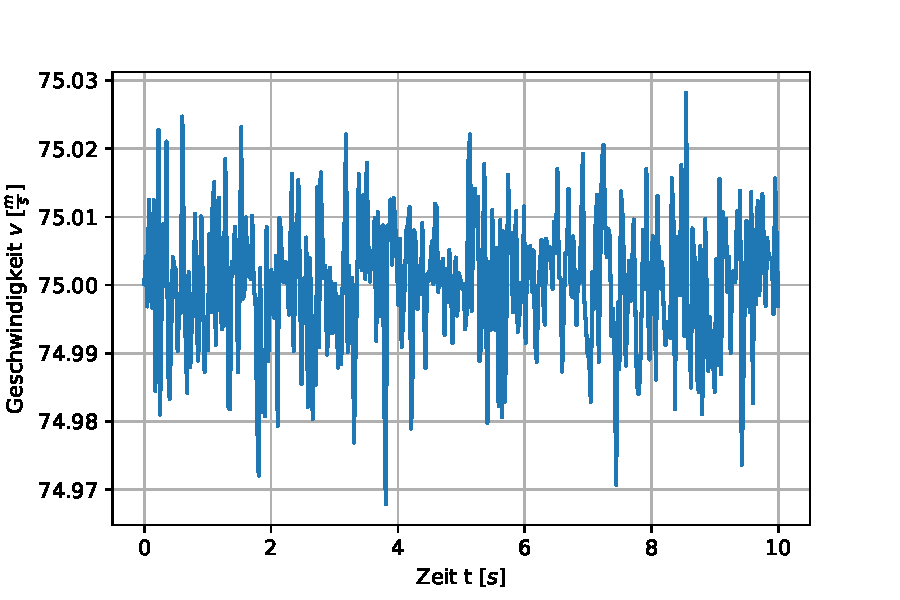
\includegraphics{fig/grundl/time/Time}
	\caption{Stetige Univariate Zeitreihe}
	\label{img:grundl:time}
\end{figure}

\FloatBarrier
\section{Dichtefunktion}
\label{sec:grundl:fkt}

Im Alltag gibt es viele Vorg�nge, deren Ergebnisse vom Zufall abh�ngig sind. Bei diesen Prozessen ist es nicht m�glich, vorherzusagen, welches Ergebnis eintritt. Man spricht bei solchen Zufallsexperimenten ebenso von nicht deterministischen Prozessen. Ein Beispiel f�r ein solches Experiment ist das Werfen eines W�rfels. Die sogenannte Ergebnismenge ist $\Omega = \{1,2,3,4,5,6\}$ und enth�lt hierbei alle m�glichen Elementarereignisse $\omega_i$, die vorkommen k�nnen. Wenn nun ein Zufallsexperiment durchgef�hrt wird, bei dem ein W�rfel zwei mal hintereinander geworfen wird, gibt es eine Menge $\mathbb{D}$, die alle m�glichen Resultate f�r die Augensumme enth�lt. In diesem Beispiel beinhaltet diese Menge alle Zahlen von $2, \ldots, 12$. Hierbei wird jede m�gliche Kombination einer Ergebnismenge $\mathbb{W}$ zugeordnet. \cite{lit:Marchthaler2017}
\\
\\
Diese Abbildung auf eine Menge erfolgt mithilfe einer Funktion, die als Zufallsvariable $X$ bezeichnet wird. Eine Zufallsvariable gilt dann als stetig, wenn sie mindestens in einem bestimmten Intervall, jeden beliebigen reellen Wert annehmen kann. Da ein endliches oder unendliches Intervall von reellen Zahlen nicht abz�hlbar unendlich viele Werte enth�lt, ist die Wahrscheinlichkeit, dass eine stetige Zufallsvariable genau einen Wert darin annimmt, gleich null. Dabei wird die Wahrscheinlichkeit, einer bestimmten Realisierung der Zufallsvariablen $X$, durch die Dichtefunktion $f(x)$ bestimmt. Diese stellt die Wahrscheinlichkeitsdichte von $X$ dar. \\F�r die Dichtefunktion gilt im Allgemeinen \cite{lit:Puhani2020}:
\begin{align}
	&\int\limits_{-\infty}^{+\infty} f(x) \,dx = 1 \quad \wedge \quad f(x) \geq 0; x \in \mathbb{R} 
	\label{eqn:dichte:def} \\
	&W(a < X \leq b) = \int\limits_{a}^{b} f(x) \,dx
	\label{eqn:dichte:prob}
\end{align}

\subsection*{\textbf{Kennzahlen}}

Mithilfe von Dichtefunktionen k�nnen Zufallsexperimente -oder variablen beschrieben werden. Allerdings gibt es noch andere Kennzahlen, die diese charakterisieren. Momente und zentrale Momente eines Zufallsexperimente z�hlen zu den wichtigsten dieser Kennwerte.

Das allgemeine $i$-te Moment ist durch
\begin{equation}
	\alpha_i = E(X^i) = \begin{cases}
		\int\limits_{-\infty}^{+\infty} x^i \cdot f_X(x) dx & \text{wenn X stetig} \\
		\sum\limits_{k \in \mathbb{N}} x(k)^i \cdot f_X(x(k)) & \text{wenn X diskret}
	\end{cases}
	\label{eqn:dichte:imom}
\end{equation}
gegeben \cite{lit:Marchthaler2017}. F�r $i = 1$ ergibt sich gem�� \autoref{eqn:dichte:imom} das erste Moment, welches ebenso als Erwartungswert $E(X)$ oder $\mu$ bekannt ist:
\begin{equation}
	\alpha_1 = E(X) = \begin{cases}
		\int\limits_{-\infty}^{+\infty} x \cdot f_X(x) dx & \text{wenn X stetig} \\
		\sum\limits_{k \in \mathbb{N}} x(k) \cdot f_X(x(k)) & \text{wenn X diskret}
	\end{cases}
	\label{eqn:dichte:1mom}
\end{equation}
Dieser trifft Aussagen �ber die Lage bzw. das Zentrum der Zufallsvariablen $X$ und stellt das gewogene arithmetische Mittel dar. In praktischen Anwendungen ist die Dichtefunktion $f_X(x)$ oft nicht bekannt, weswegen der Erwartungswert auch durch den  arithmetischen Mittelwert $\overline{x}$
\begin{equation}
	\overline{x} = \frac{1}{n} \cdot \sum\limits_{k=1}^n x(k)
	\label{eqn:dichte:mit}
\end{equation}
angen�hert wird. Die zentralen Momente einer Zufallsvariablen $X$ sind definiert durch \cite{lit:Marchthaler2017}:
\begin{equation}
	\mu_i = E\left((X - E(X))^i\right) = \begin{cases}
		\int\limits_{-\infty}^{+\infty} (X - E(X))^i \cdot f_X(x) dx & \text{wenn X stetig} \\
		\sum_{k \in \mathbb{N}} (x(k) - E(X))^i \cdot f_X(x(k)) & \text{wenn X diskret}
	\end{cases}
	\label{eqn:dichte:izmom}
\end{equation}
Das zweite zentrale Moment der Zufallsvariablen $X$
\begin{equation}
	Var(X) = E\left((X - E(X))^2\right) = \begin{cases}
		\int\limits_{-\infty}^{+\infty} (X - E(X))^2 \cdot f_X(x) dx & \text{wenn X stetig} \\
		\sum_{k \in \mathbb{N}} (x(k) - E(X))^2 \cdot f_X(x(k)) & \text{wenn X diskret}
	\end{cases}
	\label{eqn:dichte:2zmom}
\end{equation}
ergibt sich nach \autoref{eqn:dichte:2zmom} f�r $i=2$. Sie gibt eine Aussage �ber die Streuung der Verteilung einer Zufallsvariablen $X$. In diesem Kontext ist die Standardabweichung das lineare Ma� der Varianz:
\begin{equation}
	\sigma(X) = \sqrt{Var(X)}
	\label{eqn:dichte:sigma}
\end{equation}
Neben den bereits genannten Kenngr��en gibt es ebenso Formparameter, die Aussagen �ber die Gestalt von theoretischen Verteilungen machen. So gibt der Parameter
\begin{equation}
	\gamma_1 = \frac{E((X - \mu)^3)}{\sigma^3}
	\label{eqn:dichte:skew}
\end{equation}
die theoretische Schiefe der Verteilung von $X$ wieder \cite{lit:Mittag2020}. Bei $\gamma_1 = 0$ liegt eine symmetrische, bei $\gamma_1 > 0$ eine rechtsschiefe bzw. linkssteile und bei $\gamma_1 < 0$ eine linksschiefe bzw. rechtssteile Verteilung vor.
Der weitere Formparameter
\begin{equation}
	\gamma_2 = \frac{E((X - \mu)^4)}{\sigma^4}
	\label{eqn:dichte:kurtosis}
\end{equation}
gibt die theoretische W�lbung bzw. Kurtosis wieder \cite{lit:Mittag2020}. Dieser gibt an, wie stark die Flanken einer Verteilung ausgepr�gt sind bzw. wie stark die Wahrscheinlichkeitsmasse um den Erwartungswert konzentriert ist.

\subsection*{\textbf{Normalverteilung}}

Eine der wohl bekanntesten Dichtefunktionen ist die nach Carl Friedrich Gau� benannte Gau�sche Normalverteilung. Sie ist definiert durch
\begin{equation}
	f(x) = \frac{1}{\sigma \, \sqrt{2 \, \pi}} \cdot e^{- \frac{(x - \mu)^2}{2\,\sigma^2}}
	\label{eqn:dichte:gauss}
\end{equation}
mit $\mu$ als den Erwartungswert und $\sigma$ als die Standardabweichung. In \autoref{img:grundl:dichte} ist diese, f�r $\mu = 0$ und $\sigma = 1$, dargestellt (Standardnormalverteilung).

\begin{figure}
	\centering
	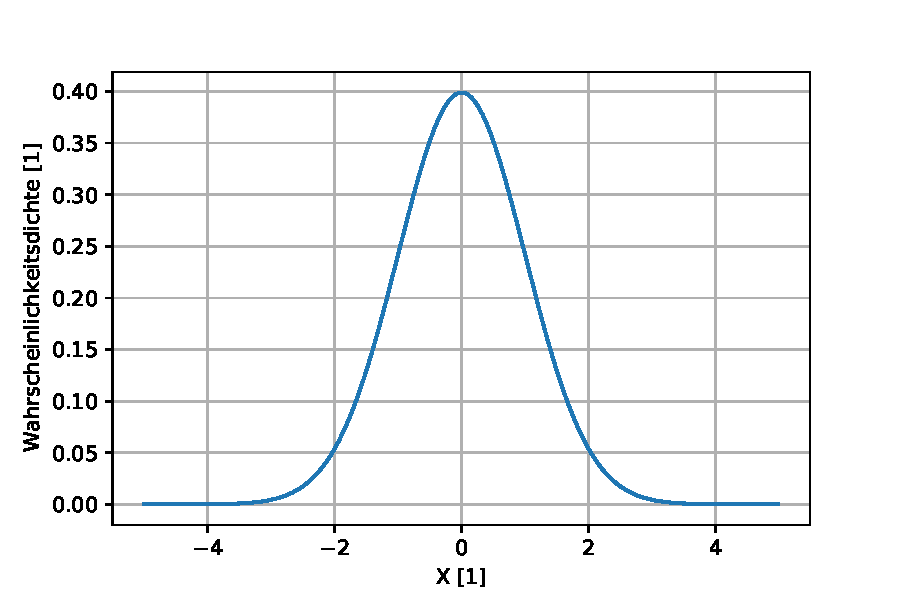
\includegraphics{fig/grundl/dichte/Dichte}
	\caption{Gau�sche Standardnormalverteilung}
	\label{img:grundl:dichte}
\end{figure}

\FloatBarrier
\subsection*{\textbf{Kerndichtesch�tzer}}

In der Praxis, wie beispielsweise bei realen Messdaten, ist die Dichtefunktion, der zugrundeliegenden Zufallsvariablen, typischerweise unbekannt. Demnach ist es wichtig, je nach Anwendungsfall, diese nicht nur qualitativ, sondern ebenso quantitativ gut abzusch�tzen. In diesem Kontext k�nnen sogenannte Kerndichtesch�tzer (\textit{engl. Kernel Density Estimator, KDE}) eingesetzt werden. Solche Kerndichtesch�tzer sind wie folgt definiert:

\begin{align}
	\tilde{f}_n(t) = \frac{1}{n h} \, \sum_{j=1}^n \, k \, \frac{(t-x_j)}{h}
	\label{eqn:dichte:kde}
\end{align}

Dabei stellt $\tilde{f}_n$ die Approximation der echten Dichtefunktion dar. Die Stichprobe ist hierbei gegeben mit $x_1, \ldots, x_n$ und der Stichprobenumfang mit $n$. Dar�ber hinaus ist die G�te des Kerndichtesch�tzers stark abh�ngig von der Bandbreite $h$. Eine zu klein gew�hlte Bandbreite bewirkt ein Overfittung der Dichtefunktion, wohingehend eine zu gro�e Bandbreite entsprechend zum Underfitting f�hrt. Gem�� dem Satz von Nadaraya existiert eine Bandbreite, so dass die approximierte Dichtefunktion gegen die echte Dichtefunktion konvergiert. Des Weiteren beinhaltet ein Kerndichtesch�tzer einen sogenannten Kernel $k$ bzw. ein Wahrscheinlichkeitsma�. Hierbei k�nnen verschiedene Kernarten verwendet werden. Der sogenannte Gau�kern (\textit{engl. Gaussian}) ist dabei wie folgt definiert:

\begin{align}
	k(t) = \frac{1}{\sqrt{2 \pi}} \, \exp{\left(-\frac{1}{2}t^2\right)}
	\label{eqn:dichte:kdegaus}
\end{align}

Sowohl die Bandbreite als auch der Kernel k�nnen mittels Optimierverfahren bestimmt werden. Dadurch wird die Berechnung der Kerndichtesch�tzer jedoch noch zeitaufw�ndiger. Je nach Genauigkeitsanforderungen und Rechenzeitaufwand k�nnen alternative Ans�tze herangezogen werden, um die Wahrscheinlichkeitsdichtefunktion abzusch�tzen. Beispielsweise mittels einer sogenannten Histogramm-Spline-Approximation. Hierbei wird eine Spline durch das Histogramm, der zugrundeliegenden Daten, gelegt. Eine solche Approximation erf�llt ebenso die wesentlichen Eigenschaften einer  Wahrscheinlichkeitsdichtefunktion. Die Histogramm-Spline-Approximation ist insbesondere vom Grad der Spline und der Anzahl der Bins des Histogrammes abh�ngig. \cite{lit:Schick2021}

\section{Evaluierungstechniken von generativen Algorithmen}
\label{sec:grundl:eval}

Gem�� \autoref{sec:grundl:gan} lassen sich synthetische Daten mithilfe von generativen Algorithmen erzeugen. Grunds�tzlich k�nnen diese generierten Daten mit dem Ausgangsdatensatz, auf visueller bzw. qualitativer Ebene, verglichen werden. Ein quantitativer Ansatz ist hingegen der Vergleich der beiden Wahrscheinlichkeitsdichtefunktionen. Hierzu gibt es eine Vielzahl verschiedenster Evaluierungstechniken. Darunter f�llt die statistische Distanz zweier Dichtefunktionen. Im Folgenden wird dieser Begriff, auf Basis der Arbeit von M. Deza und E. Deza \cite{lit:Deza2013}, n�her erl�utert.
\\
\\
Eine Distanz (\textit{engl. Distance oder Dissimilarity}) $d(x,y)$ ist eine Funktion, die eine Menge $X$ auf den reellen Raum abbildet, \dah $d : \, X \times X \rightarrow \mathbb{R}$. Hierbei werden $x,y \in X$ durch $d$ auf den reellen Raum abgebildet. Diese besitzt folgende Eigenschaften:
\begin{align*}
	d(x,y) &\geq 0 \qquad & (Nicht-Negativit�t) \\
	d(x,y) &= d(y,x) \qquad & (Symmetrie) \\
	d(x,x) &= 0 \qquad & (Reflexivit�t) \\
\end{align*}
Eine weitere Art, die Diskrepanz zweier Dichtefunktionen zu bestimmen, ist die �hnlichkeit (\textit{engl. Similarity}). �hnlich wie eine Distanz, bildet diese eine Menge auf den reellen Raum ab, \dah $s : \, X \times X \rightarrow \mathbb{R}$. Neben den Eigenschaften Nicht-Negativit�t und Symmetrie, muss f�r eine Similarity gelten $s(x,y) \leq s(x,x)$ f�r alle $x,y \in X$, au�er f�r $y=x$. Similarities $s$ und Distances $d$ k�nnen durch verschiedene Transformationen ineinander umgeformt werden. Beispielsweise durch: $d = 1 - s$, $d = \frac{1 - s}{s}$, $d = \sqrt{1 - s}$ oder $d = -\ln(s)$ \cite{lit:Deza2013}. Umso �hnlicher sich $x$ und $y$ sind, desto h�her ist der Wert einer Similarity $s$. Im Gegensatz ist eine Distanz $d$ umso geringer, desto �hnlicher sich $x$ und $y$ sind. In beiden F�llen k�nnen die dazugeh�rigen Kennzahlen normalisiert werden. Dann gilt $0 \leq s(x,y) \leq 1$ bzw. $0 \leq d(x,y) \leq 1$.
\newpage
Die Definition einer Distanz kann in eine Semi-Metrik erweitert werden. Hierzu muss, zus�tzlich zur Nicht-Negativit�t, Symmetrie und Reflexivit�t, f�r alle $x,y,z \in X$ gelten:
\begin{align*}
	d(x,y) &\leq d(x,z) + d(z,y) \qquad & (Dreiecksungleichung)
\end{align*}
Eine Metrik erweitert die Semi-Metriken zus�tzlich um die Identit�t (\textit{engl. identity}):
\begin{align*}
	d(x,y) &\geq 0 \qquad & (Nicht-Negativit�t) \\
	d(x,y) &= 0 \Leftrightarrow x=y \qquad & (Identit�t) \\
	d(x,y) &= d(y,x) \qquad & (Symmetrie) \\
	d(x,y) &\leq d(x,z) + d(z,y) \qquad & (Dreiecksungleichung)
\end{align*}
Eine Menge $X$, inkl. einer Metrik $d$, wird als metrischer Raum $(X,d)$ bezeichnet. Diese Evaluierungstechniken bilden den Rahmen, um Dichtefunktionen, im Kontext von generativen Algorithmen, miteinander zu vergleichen. Distanzen, die asymmetrisch sind, k�nnen in symmetrische transformiert werden. In \autoref{tab:grundl:eval} befinden sich einige dieser Transformationen \cite{lit:Cha2007}. 
\begin{table}[h!]
	\centering
	\begin{tabular}{p{0.4\linewidth}|p{0.55\linewidth}}
		\toprule
		\textbf{Methode} & \textbf{Beschreibung} \\ 
		\midrule
		Addition & $d_{sym}(\mathbb{P},\mathbb{Q}) = d_{asym}(\mathbb{P},\mathbb{Q}) + d_{asym}(\mathbb{Q},\mathbb{P})$ \\
		\midrule
		Maximum  & $d_{max-sym}(\mathbb{P},\mathbb{Q}) = \max\left(d_{asym}(\mathbb{P},\mathbb{Q}),d_{asym}(\mathbb{Q},\mathbb{P})\right)$ \\
		\midrule
		Minimum   & $d_{min-sym}(\mathbb{P},\mathbb{Q}) = \min\left(d_{asym}(\mathbb{P},\mathbb{Q}),d_{asym}(\mathbb{Q},\mathbb{P})\right)$ \\
		\midrule
		Durchschnitt & $d_{avg-sym}(\mathbb{P},\mathbb{Q}) = avg\left(d_{asym}(\mathbb{P},\mathbb{Q}),d_{asym}(\mathbb{Q},\mathbb{P})\right)$ \\
		\bottomrule
	\end{tabular}
	\caption{Techniken zur Symmetrisierung einer Distanz}
	\label{tab:grundl:eval}
\end{table}

\chapter{Hauptteil}
\label{sec:real}
Dieses Kapitel beschreibt den Hauptteil der zugrundeliegenden Arbeit. Hierbei werden, in einem ersten Schritt, der Anwendungsfall sowie die genaue Herangehensweise, bei der umfangreichen Literaturrecherche, n�her erl�utert. Anschlie�end wird eine neuartige Taxonomie der Evaluierungstechniken von Wahrscheinlichkeitsdichtefunktionen vorgestellt, die zur Validierung von generativen Algorithmen, im Kontext der Bereitstellung von zeitreihen-bezogenen Daten, verwendet werden k�nnen. Weiterhin wird jede einzelne Evaluierungstechnik in der engeren Auswahl n�her beschrieben. Daraufhin werden definierte Bewertungskriterien f�r eine Gegen�berstellung der Methoden vorgestellt. Abschlie�end erfolgt die Implementierung und Validierung einer ausgew�hlten Evaluierungstechnik anhand von synthetisch erzeugten Beispieldatens�tzen.

\section{Anwendungsfall}
\label{sec:haupt:anwendung}

Wie in \autoref{sec:grundl:af} bereits beschrieben wurde, m�ssen autonome Fahrzeuge mit jeder Situation im Stra�enverkehr umgehen k�nnen. Darunter fallen ebenso fahrkritische Szenarien, wie �berhol- oder Abbiegevorg�nge. In \autoref{img:haupt:ueberhol} ist ein solcher �berholvorgang beispielhaft dargestellt.

\begin{figure}
	\centering
	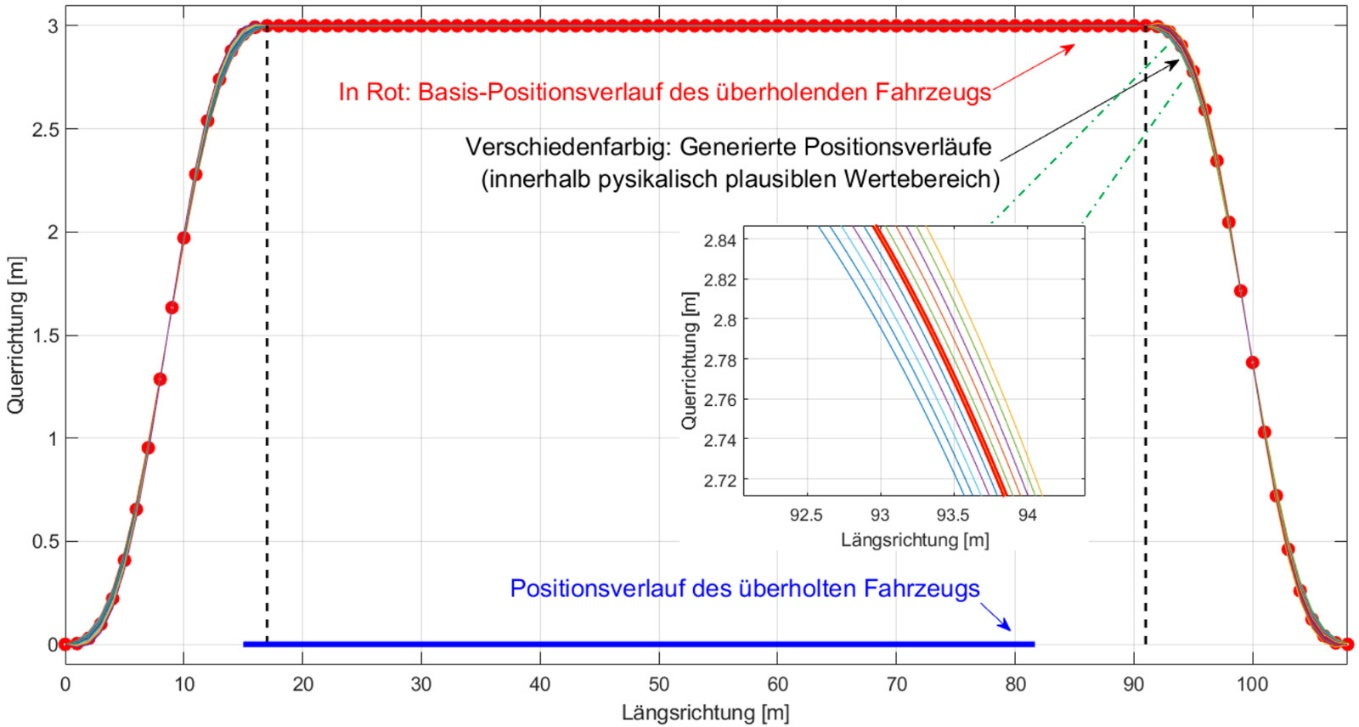
\includegraphics{fig/haupt/Ueberholvorgang}
	\caption{�berholvorgang}
	\label{img:haupt:ueberhol}
\end{figure}

Hierbei sind im Koordinatensystem die Bewegungsdaten der Fahrzeuge, f�r die L�ngs- und Querrichtung, dargestellt. Der Positionsverlauf des �berholten Fahrzeugs ist in blau aufgezeigt. Die rote Kurve stellt den Verlauf des �berholenden Fahrzeugs dar. Der gesamte �berholvorgang erstreckt sich �ber eine Strecke von 110 m in L�ngs- sowie 3 m in Querrichtung. Die roten Datenpunkte, auf der Kurve des �berholenden Fahrzeugs, zeigen die einzelnen Zeitstempel. Hierbei ist anzumerken, dass die Anzahl der Datenpunkte, f�r den Ein- und Ausschervorgang, geringer ist, als f�r den restlichen Verlauf. Dies liegt daran, dass die zur�ckgelegte Strecke in Querrichtung, f�r diese Verl�ufe, geringer ist, als f�r den eigentlichen �berholvorgang. In der Vergr��erung sind generierte synthetische Positionsverl�ufe aufgezeigt. Diese befinden sich innerhalb eines physikalisch plausiblen Wertebereich.
\\
\\
Um die Algorithmen von autonomen Fahrzeugen, f�r diese F�lle, trainieren zu k�nnen, m�ssen Daten, f�r diese, vorhanden sein. In der Realit�t sind etwaige Realdaten bzw. Messungen kaum vorhanden. Gr�nde hierf�r sind das geringe Auftreten solcher Szenarien oder die seltene Aufnahme dieser, aufgrund der zugrundeliegenden Kritikalit�t. Eine Abhilfe kann hier die Verwendung von generativen Algorithmen sein, die synthetische Daten generieren k�nnen. Durch die Verwendung dieser synthetischen Daten, ist es m�glich, autonome Fahrzeuge, f�r diese fahrkritischen Szenarien, zu trainieren.
%Motivation aufgreifen/wiederholen: geringe Daten f�r fahrkritische Szenarien in der Realit�t --> synthetische Daten mithilfe von generativen Algorithmen
\\
\\
Die Daten in Kraftfahrzeugen, die in solchen fahrkritischen Szenarien anfallen, sind zumeist Sensordaten. Diese werden \zB in Bewegungsvektoren zusammengefasst und enthalten Daten u.a. �ber die Zeit, Geschwindigkeit, Beschleunigung und Position in x- und y-Richtung. Gem�� der Unterscheidung in \autoref{sec:grundl:time}, bilden diese Art von Daten periodische, multivariate Zeitreihen. Im zugrundeliegenden Anwendungsfall haben diese Bewegungsvektoren ebenso die gleiche L�nge. Einerseits gehen Informationen verloren, falls etwaige  Datenpunkte entfernt werden. Andererseits k�nnen fehlende Datenpunkte, nicht f�r jeden Fall, kinematisch korrekt nachgebildet werden.
%Anwendungsfall beschreiben: Daten sind periodische, multivariate Zeitreihen (Sensordaten) --> Bewegungsvektoren (Zeit, Position in x, y, Geschwindigkeit, Beschleunigung) mit gleicher L�nge --> nicht Zeitreihen schneiden und nicht hinzuf�gen mit 0, man ist nicht mehr kinematisch
\\
\\
In generativen Algorithmen werden, wie in \autoref{sec:grundl:gan} beschrieben, Dichtefunktionen verwendet, um Datens�tze abzubilden und zu generieren. Es liegen jeweils 100 Datens�tze zu ausgew�hlten Szenarien vor. Darunter z�hlen entsprechende Bewegungsvektoren inkl. Dichtewerte zur Sinusfunktion und zum �berholman�ver mit Gegenverkehr. Die in den Datens�tzen befindlichen Dichtefunktionswerte sollen miteinander verglichen werden. Dazu soll eine entsprechende Evaluierungstechnik verwendet werden. Dadurch kann eine Kennzahl bzw. ein Ma� ermittelt werden, welche die �bereinstimmung der Dichtefunktionen darstellt. Mithilfe einer solchen Kennzahl ist es m�glich, zu entscheiden, ob die synthetisch erzeugten Daten, tats�chlich fahrkritische Szenarien abbilden.
%Zwei Dichtefunktionen f�r jedes fahrkritisches Szenario --> f�r 100 Samples eine Dichtefunktion --> Realdaten pdf vergleichen mit GAN pdf , Input sind 4 Parameter --> 2 Vektoren je pdf mit jeweils x,y
%Eine Kennzahl rausfinden mithilfe von Evaluierungstechnik: damit Threshold definieren, um nicht synthetisch fahrkritische Szenarien auszusortieren, muss nicht normiert sein auf [ 1,1] oder [0,1]

\section{Vorgehensweise}
\label{sec:haupt:vorgehen}

Dichtefunktionen k�nnen auf verschiedenste Arten und Weisen bewertet, evaluiert oder validiert werden. In diesem Kontext existieren eine Vielzahl an Publikationen. Deshalb erfolgte eine systematische Vorgehensweise, um die relevanten Publikationen zu finden. Hierzu wurden spezielle Suchstrings erstellt, die relevante Stichw�rter enthalten. Dabei erfolgten ebenso Permutationen der einzelnen Stichw�rter, um ein gr��eres Spektrum an Suchergebnissen zu erhalten. \newpage Die Suchstrings wurden anschlie�end in Gruppen eingeteilt und dienten als Basis f�r die Literaturrecherche. Insgesamt erfolgte die beschriebene Literaturrecherche ausschlie�lich �ber Suchmaschinen im Internet. 
\\
\\
Um die Relevanz der gefundenen Publikationen einzustufen, wurde in einem ersten Schritt, die jeweiligen Einleitungs- und Zusammenfassungs-Kapitel gelesen. Diese geben einen guten �berblick �ber die zugrundeliegenden Publikationen. Entsprechende Evaluierungstechniken, die in den Publikationen genannt und beschrieben werden, wurden extrahiert und in einer Liste gesammelt. In einem weiteren Schritt wurden die Publikationen n�her betrachtet. Dadurch sind, die f�r den Anwendungsfall irrelevanten Evaluierungstechniken, weiter ausgefiltert worden. Im n�chsten Schritt erfolgte eine Gruppierung von �hnlichen Evaluierungstechniken. Damit konnte eine eigene Taxonomie an Evaluierungstechniken, f�r den zugrundeliegenden Anwendungsfall, erstellt werden. Diese werden sp�ter, anhand von festgelegten Bewertungskriterien, evaluiert.

\section{Taxonomie der Evaluierungstechniken von Wahrscheinlichkeitsdichtefunktionen}
\label{sec:haupt:taxonomie}

Durch die Literaturrecherche ergab sich eine umfangreiche Liste an m�glichen Evaluierungstechniken. Diese wurden in bestimmte Teilbereiche zusammengefasst, um eine Taxonomie zu bilden. Die zugrundeliegende mathematische Beschreibung dieser Evaluierungstechniken, war die Basis f�r diese Unterteilung. In \autoref{img:haupt:taxonomie} ist diese Taxonomie dargestellt.
\begin{figure}[h!]
	\centering
	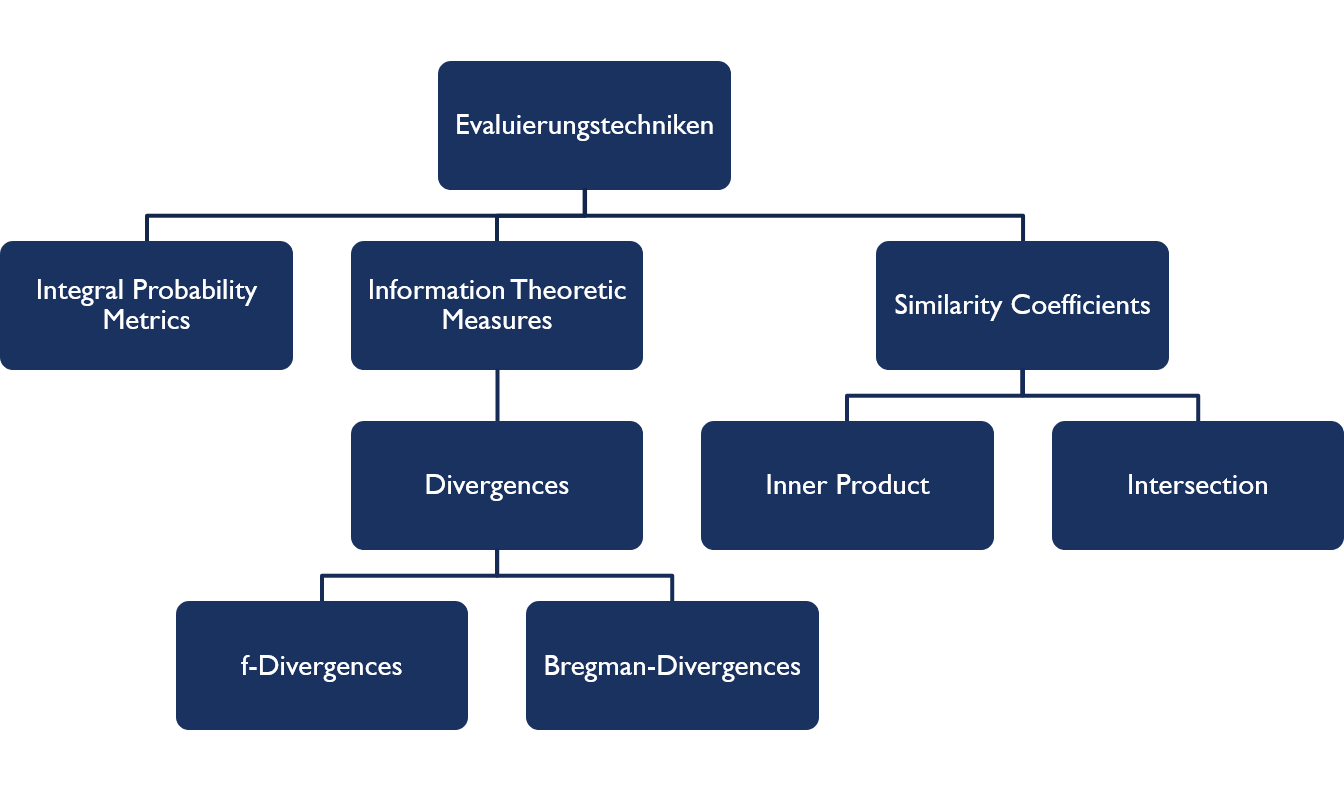
\includegraphics[width=\linewidth]{fig/haupt/tax/taxonomie}
	\caption{Taxonomie von Evaluierungstechniken in Bezug auf Dichtefunktions-Vergleiche}
	\label{img:haupt:taxonomie}
\end{figure}
\\
\\
Eine essenzielle Gruppe an Evaluierungstechniken bilden die Integral Probability Metrics. Die grundlegende Struktur dieser Metriken bildet die Differenz zweier Wahrscheinlichkeitsma�e $\mathbb{P}$ und $\mathbb{Q}$. Sie sind wie folgt definiert \cite{lit:Gardner2018}:
\begin{equation}
	\gamma_F(\mathbb{P},\mathbb{Q}) := \sup\limits_{f \in \mathcal{F}}\left| \int f \,d\mathbb{P} - \int f \,d\mathbb{Q}\right|
	\label{eqn:tax:ipm} 
\end{equation}
Hierbei ist die Funktion $f$ einer Klasse von reellen und beschr�nkten Funktionen $\mathcal{F}$ zugeh�rig.
\\
\\
Eine weitere wichtige Gruppe an Evaluierungstechniken bilden informationstheoretische Ma�e. Eine essenzielle historische Kennzahl, in diesem Bereich, ist die Entropie. Diese ist ein Ma� �ber den Informationsgehalt bzw. die Unsicherheit einer Zufallsvariablen $X$. Sie ist wie folgt definiert \cite{lit:entropy:Csiszar2008}:
\begin{equation}
	H(X) = -\sum\limits_{i = 1}^N x_i \cdot \log_2(x_i),\ i=1,\ldots,N
	\label{eqn:tax:entropie}
\end{equation}
Viele statistische Distanzen basieren auf der Entropie. Ein ebenfalls bedeutendes Mittel zum Vergleich von Dichtefunktionen sind Divergenzen bzw. Divergenzma�e (\textit{engl. Divergences}). Hierbei ist anzumerken, dass viele der Evaluierungstechniken, wie \zB Divergenzen, keine Metriken, wie in \autoref{sec:grundl:eval} definiert, darstellen. Das schlie�t sie jedoch nicht als passendes Evaluierungsmittel aus. Die hohe Anzahl an Nennungen in Literaturen rechtfertigt die Relevanz dieser Evaluierungstechniken f�r den zugrundeliegenden Anwendungsfall.
\\
\\
Eine der wohl bekanntesten Familie an Divergenzma�en ist die $f$-Divergence. Diese beinhaltet eine hohe Anzahl an bekannten statistischen Distanzen. Sie ist definiert durch:
\begin{equation}
	d_f(p,q) = \sum\limits_{x} q(x)f\left(\frac{p(x)}{q(x)}\right)
	\label{eqn:tax:fdiv}
\end{equation}
Hierbei ist $f$ eine beliebige Funktion, die konvex �ber dem Definitionsbereich $(0,\infty)$ ist und f�r die gilt $f(1) = 0$. Des Weiteren sind $f$-divergences stets nicht-negativ und nur dann null, wenn die zwei Dichtefunktionen $p(x)$ und $q(x)$ �bereinstimmen \cite{lit:fdiv:Cichocki2010}. 
\\
\\
Eine weitere wichtige Gruppe von Evaluierungstechniken sind die Bregman-Divergenzen. Diese messen die Diskrepanz zwischen zwei Werten von Dichtefunktionen $p(x)$ und $q(x)$ \cite{lit:fdiv:Cichocki2010}:
\begin{equation}
	d_\varphi(p,q) = \varphi(p) - \varphi(q) - (p - q)\varphi'(q)
	\label{eqn:tax:bregman}
\end{equation}
Die gesamte Diskrepanz zwischen den Dichtefunktionen $p(x)$ und $q(x)$, l�sst sich, mit Hilfe der Bregman-Divergenz, wie folgt beschreiben:
\begin{equation}
	d_\varphi(\mathbb{P},\mathbb{Q}) = \int\left[\varphi(p(x)) - \varphi(q(x)) - (p(x) - q(x))\varphi'(q(x))\right] \,dx
	\label{eqn:tax:bregmancont}
\end{equation}
\autoref{eqn:tax:bregmancont} l�sst sich, wie in folgender Rechenvorschrift, diskretisieren:
\begin{equation}
	d_\varphi(\mathbb{P},\mathbb{Q}) = \sum\limits_{i = 1}^N\left[\varphi(p_i) - \varphi(q_i) - (p_i - q_i)\varphi'(q_i)\right]
	\label{eqn:tax:bregmandiskret}
\end{equation}
Hierbei muss die Funktion $\varphi(t)$ streng konvex und reell sein. $\varphi'(\mathbb{Q})$ beschreibt die Ableitung nach $\mathbb{Q}$. Bregman-Divergenzen besitzen ebenso die Eigenschaft der Nicht-Negativit�t (vgl. \autoref{sec:grundl:eval}). Die Symmetrie ist abh�ngig von $\varphi(t)$. 
\\
\\
Mithilfe von sogenannten Similarity Coefficients k�nnen ebenso zwei Dichtefunktionen, in Bezug auf ihrer �hnlichkeit, miteinander verglichen werden. Hierbei werden die beiden Dichtefunktionen bzw. Datens�tze $\mathbb{P}$ und $\mathbb{Q}$, mittels unterschiedlichen Operationen, gegen�bergestellt. Zu diesen z�hlen Kennzahlen, die auf dem Inner Product oder der Intersection basieren. Folgende Definitionen beruhen auf den Erkenntnissen in \cite{lit:Cha2007}.
\\
\\
Hierzu z�hlen unter anderem Kennzahlen, die auf dem Inner Product basieren. Hierbei treten die zwei Dichtefunktionen $P$ und $Q$ in der folgenden Form auf:
\begin{equation}
	s = P \bullet Q = \sum\limits_{i=1}^d = P_iQ_i
	\label{eqn:tax:dot}
\end{equation}
Das Inner Product von zwei Vektoren wird ebenso als Skalarprodukt bezeichnet.
\\
\\
Des Weiteren gibt es noch Kennzahlen, die auf der �berschneidung von Dichtefunktionen aufbauen. In der Form einer Similarity treten diese wie folgt auf:
\begin{equation}
	s = \sum\limits_{i=1}^N\min(P_i,Q_i)
	\label{eqn:tax:sintersection}
\end{equation}
Durch die bereits in \autoref{sec:grundl:eval} genannte Umformung $d = 1 - s$, l�sst sich die Intersection ebenso als Distanz formulieren:
\begin{equation}
	d = \frac{1}{2}\sum\limits_{i=1}^N|P_i - Q_i|
	\label{eqn:tax:dintersection}
\end{equation}

\section{Mathematische Beschreibung der Evaluierungstechniken von Wahrscheinlichkeitsdichtefunktionen}
\label{sec:haupt:math}

%\subsection{Telescope Distance}
%\label{sec:haupt:telescope}
%\workTodo{}
%
%\subsection{Jaccard Coefficient}
%\label{sec:haupt:jaccardcoeff}
%\workTodo{}
%
%\subsection{Dice Coeffiecient}
%\label{sec:haupt:dice}
%\workTodo{}
%
%\subsection{Wave Hedges}
%\label{sec:haupt:wave}
%\workTodo{}
%
%\subsection{Czekanowski Coefficient}
%\label{sec:haupt:czekanowski}
%\workTodo{s -> d: sorensen/bray-curtis/canberra, 0.5:Motyka}
%
%\subsection{Jaccard und Tanimoto Distance}
%\label{sec:haupt:tanimoto}
%\workTodo{1 - d: ruzicka}
%
%\subsection{Lorentzian Coefficient}
%\label{sec:haupt:lotrentzian}
%\workTodo{}

Im Folgenden werden einige Evaluierungstechniken bzw. Algorithmen, gem�� ihrer Definition, diskret oder kontinuierlich beschrieben.
%\workTodo{Levy, Pro(k)horov, Inception -> Mode Sore, Fr�chet Inception, Area Validation Metric}
\subsection{Kolmogorov-Smirnov Metrik}
\label{sec:haupt:kolmogorov}

Die Kolmogorov-Smirnov Distanz - oder auch Kolmogorov-Smirnov Metrik - geh�rt zu der Familie der Integral Probability Metrics.
Sie ist, im Normalfall, als die $L_1$ Norm (vgl. \autoref{sec:haupt:minkowski}) zwischen zwei kumulativen Dichtefunktionen definiert:
\begin{equation}
	d_{KS}(\mathbb{P},\mathbb{Q}) = \sup\limits_{x \in \mathbb{R}} \left|F_p(x) - F_q(x)\right|
	\label{eqn:math:kscont}
\end{equation}
In \autoref{eqn:math:kscont} stehen $\mathbb{P}$ und $\mathbb{Q}$ f�r kumulative Verteilungsfunktionen und $sup$ f�r die Supremum Funktion. Diese gibt die kleinste obere Schranke einer Punktedifferenz, also die maximale Differenz, wieder. Zus�tzlich ist die Kolmogorov-Smirnov Distanz auf $[0,1]$ beschr�nkt, wodurch das Ergebnis leichter interpretiert werden kann. Sie wird, im Normalfall, dazu verwendet, um einen Kolmogorov-Smirnov Test durchzuf�hren. Hierbei werden zwei eindimensionale kumulative Verteilungsfunktionen verglichen. Dies geschieht durch den Hypothesentest $F_p(x) = F_q(x)$ \cite{lit:Gardner2018}.
In diskreter Form und auf Dichtefunktionen bezogen, l�sst sich diese, basierend auf \cite{lit:Rubner2000}, wie folgt definieren:
\begin{equation}
	d_{KS}(\mathbb{P},\mathbb{Q}) = \max\limits_{i}(\left|p_i - q_i\right|)
	\label{eqn:math:ksdiskret}
\end{equation}
Hierbei kann, f�r diskrete Dichtefunktionen, die jeweilige kumulative Verteilungsfunktion iterativ berechnet werden. F�r den diskreten Fall ist sie somit �hnlich aufgebaut wie die $L_\infty$ Metrik (vgl. \autoref{eqn:math:Linf}). Die Kolmogorov-Smirnov Distanz entspricht, im Falle von diskreten kumulativen Verteilungen, dem maximalen Abstand zwischen $\mathbb{P}$ und $\mathbb{Q}$. Sie eignet sich somit nicht f�r Datens�tze oder Dichtefunktionen mit Ausrei�ern.
\subsection{Wasserstein Distance}
\label{sec:haupt:wasserstein}

Die Wasserstein-1 Distance ist ein Ma� f�r die Distanz zwischen zwei Dichtefunktionen. Sie wird ebenso als die Earth Mover's (EM) Distance bezeichnet. Sie ist definiert durch \cite{lit:Weng2019}:
\begin{equation}
	W(\mathbb{P},\mathbb{Q}) = \inf\limits_{\gamma \in \prod(\mathbb{P},\mathbb{Q})} \mathbb{E}_{(x,y) \sim \gamma} \left[\parallel x - y\parallel\right]
	\label{eqn:math:wasserstein1}
\end{equation}
In \autoref{eqn:math:wasserstein1} ist $\prod(\mathbb{P},\mathbb{Q})$ die Menge aller gemeinsamen Wahrscheinlichkeitsverteilungen zwischen $\mathbb{P}$ und $\mathbb{Q}$. $\gamma \in \prod(\mathbb{P},\mathbb{Q})$ beschreibt eine der Transformationen, um $\mathbb{P}$ in $\mathbb{Q}$ zu �berf�hren. Die EM-Distanz stellt die \textqu{Kosten} dar.
Mit Hilfe der Kantorovich-Rubinstein Dualit�t l�sst sich die Wasserstein Distanz ebenso als Integral Probability Metric, wie folgt, definieren \cite{lit:Arjovsky2017}:
\begin{equation}
	W(\mathbb{P},\mathbb{Q}) = \sup\limits_{\parallel f \parallel_L \leq 1} \mathbb{E}_{x \sim \mathbb{P}} \left[f(x)\right] - \mathbb{E}_{x \sim \mathbb{Q}} \left[f(x)\right]
	\label{eqn:math:wassersteinipm}
\end{equation}
In \autoref{eqn:math:wassersteinipm} umfasst die Menge der Funktionen $\mathcal{F}$ (vgl. \autoref{eqn:tax:ipm}) alle 1-Lipschitz Funktionen. Der Ausdruck $\mathbb{E}_{(x,y) \sim P}\left[f(x)\right]$ stellt den Erwartungswert in Bezug auf die Verteilung $P$ der Funktion $f(x)$ dar. Analog dazu l�sst sich der Ausdruck $\mathbb{E}_{(x,y) \sim Q}\left[f(x)\right]$ erkl�ren. Es ist zu beachten, dass die Definition einer Integral Probability Metric, von der in \autoref{eqn:tax:ipm}, abweicht. Der �bergang von Integralen zu Erwartungswerten erfolgt �hnlich wie in \autoref{eqn:dichte:imom}.

\subsection{Cram�r Distance}
\label{sec:haupt:cramer}

Eine weitere Integral Probability Metric ist die Cram�r Distance \cite{lit:Bellemare2017}. Diese ist definiert durch:
\begin{equation}
	L_2^2(\mathbb{P},\mathbb{Q}) := \int\limits_{-\infty}^{\infty}(F_P(x) - F_Q(x))^2 \,dx
	\label{eqn:math:cramer}
\end{equation}
In \autoref{eqn:math:cramer} ist zu erkennen, dass die Cram�r Distance keine vollwertige Metrik darstellt. Allerdings stellt ihre Wurzel eine dar und geh�rt zur $L_P$ Familie der Metriken (vgl. \autoref{sec:haupt:minkowski}).
\subsection{Minkowski}
\label{sec:haupt:minkowski}

Die Minkowski Metrik stellt die Familie der $L_p$ Metriken dar. Sie ist definiert durch \cite{lit:Bellemare2017}:
\begin{equation}
	L_p(\mathbb{P},\mathbb{Q}) := \left(\int\limits_{-\infty}^{\infty}\left|F_P(x) - F_Q(x)\right|^p \,dx\right)^{\frac{1}{p}}
	\label{eqn:math:minkowskicont}
\end{equation}
F�r den diskreten Fall kann sie, wie folgt, beschrieben werden \cite{lit:Cha2007}:
\begin{equation}
	d_{L_p}(\mathbb{P},\mathbb{Q}) = \sqrt[p]{\sum\limits_{i = 1}^{n} \left|P_i - Q_i\right|^p}
	\label{eqn:math:minkowskidiskret}
\end{equation}
Die Minkowski Metrik ist eine Verallgemeinerung von verschiedenen anderen Distanzen. Diese ergeben sich durch die entsprechenden Werte f�r den Parameter $p$. Beispielsweise f�hrt $p = 1$ zur $L_1$ Metrik. Diese wird ebenso als City-Block oder Manhattan-Distanz bezeichnet:
\begin{equation}
	d_{L_1}(\mathbb{P},\mathbb{Q}) = \sum\limits_{i = 1}^{N} \left|P_i - Q_i\right|
	\label{eqn:math:L1}
\end{equation}
Durch die Wahl $p = 2$ ergibt sich die Euklidische Distanz:
\begin{equation}
	d_{L_2}(\mathbb{P},\mathbb{Q}) = \sqrt[2]{\sum\limits_{i = 1}^{N} \left|P_i - Q_i\right|^2}
	\label{eqn:math:L2}
\end{equation}
F�r $p = \infty$ ergibt sich die Chebyshev-Distanz, die als die maximale Differenz zweier Datens�tze definiert ist:
\begin{equation}
	d_{L_{\infty}}(\mathbb{P},\mathbb{Q}) = \max\limits_{i}\left|P_i - Q_i\right|
	\label{eqn:math:Linf}
\end{equation}
Grundlegend l�sst sich sagen, dass durch die Wahl eines h�heren Werts f�r $p$, die gr��te Distanz bzw. Differenz zweier Elemente h�her gewichtet wird. Es ist der Zusammenhang zwischen den $L_p$ und Wasserstein Metriken anzumerken. F�r den Fall $p = 1$ sind diese identisch. Ebenso wie Wasserstein Metriken, k�nnen $L_p$ Metriken, in der Form einer Integral Probability Metric, beschrieben werden \cite{lit:Bellemare2017}:
\begin{equation}
	d_{Mk}(\mathbb{P},\mathbb{Q}) = \sup\limits_{f \in \mathbb{F}_q}\left|\mathbb{E}_{x \sim P}f(x) - \mathbb{E}_{x \sim Q}f(x)\right|
	\label{eqn:math:minkowskiipm}
\end{equation}
In \autoref{eqn:math:minkowskiipm} wird hier das Supremum �ber die absolut stetigen Funktionen $\mathbb{F}_q$ gebildet. Der Ausdruck $\mathbb{E}_{x \sim P}f(x)$ stellt den Erwartungswert in Bezug auf die Verteilung $P$ der Funktion $f(x)$ dar. Analog dazu l�sst sich der Ausdruck $\mathbb{E}_{x \sim Q}f(x)$ erkl�ren.

\subsection{Maximum Mean Discrepancy}
\label{sec:haupt:maxmeandiscrepancy}

Die Maximum Mean Discrepancy (MMD) geh�rt zur Klasse der Integral Probability Metrics, wenn in \autoref{eqn:tax:ipm} f�r $\mathcal{F} = \left\{ f :\, \parallel f \parallel_{\mathcal{H}} \,\leq\, 1\right\}$ gilt, wobei $\mathcal{H}$ den reproduzierenden Kernel Hilbertraum (\textit{engl.: Reproducing Kernel Hilbert Space (RKHS)}) bezeichnet. Sie bewertet die Differenz zweier Distributionen mit Hilfe einer Gl�ttungsfunktion. Diese Funktion erzeugt f�r Stichproben aus $\mathbb{P}$ gro�e und f�r $\mathbb{Q}$ kleine Werte. F�r Samples $x$ und $y$, entsprechend aus $\mathbb{P}$ und $\mathbb{Q}$, ist die MMD wie folgt definiert \cite{lit:Gardner2018}:
\begin{equation}
	d_{MMD}(\mathbb{P},\mathbb{Q}) = \sup\limits_{f \in \mathcal{F}}\left|\mathbb{E}_x\left[f(x)\right] - \mathbb{E}_y\left[f(y)\right]\right|
	\label{eqn:math:mmd}
\end{equation}
Die \autoref{eqn:math:mmd} liefert Werte f�r die beiden Stichproben, wobei die Differenz zwischen den Mittelwerten dieser Funktionswerte, dem MMD entspricht. D.\, h. dem maximalen Abstand zwischen den Mittelwerten nach der Transformation durch die Gl�ttungsfunktion $f$. Zu der Funktionsklasse $\mathcal{F}$ geh�ren alle Funktionen, die einen RKHS produzieren, sogenannte reproduzierende Kernels. Es gibt eine Reihe von Kernels $k(\cdotp,\cdotp)$, die in der MMD gew�hlt werden k�nnen. Eine beliebte Wahl ist der radiale Basiskernel: 
\begin{equation}
	k(x,x') = e^{\frac{\parallel x - x'\parallel^2}{2\sigma^2}}
	\label{eqn:math:mmdkernel}
\end{equation}
Hierbei sind $x$ und $x'$ jeweils Samples aus den entsprechenden Dichtefunktionen $p(x)$ und $q(x)$. Der Parameter $\sigma$ wird oft durch den Median der paarweisen Abst�nde zwischen den gemeinsamen Daten bestimmt.

\subsection{Total Variation Metric}
\label{sec:haupt:totalvariation}

Die Total Variation Metric nimmt eine besondere Stellung unter den Evaluierungstechniken ein. Sie kann zum einen, durch die Wahl von $f(t) = \frac{\left|t - 1\right|}{2}$ in \autoref{eqn:tax:fdiv}, als $f$-Divergence beschrieben werden. Zum anderen kann sie, durch die Wahl von $\mathcal{F} = \left\{ f :\, \parallel f \parallel_{\infty} \,\leq\, 1\right\}$ in \autoref{eqn:tax:ipm}, als Integral Probability Metric definiert werden.
Eine M�glichkeit, diese zu beschreiben, ist wie folgt \cite{lit:Gardner2018}:
\begin{equation}
	d_{TV}(\mathbb{P},\mathbb{Q}) = \sqrt{\frac{1}{2}\int\left|p(x) - q(x)\right|\,dx}
	\label{eqn:math:tv}
\end{equation}
Es ist anzumerken, dass der Wertebereich der Gleichung \autoref{eqn:math:tv} auf $\left[0,1\right]$ beschr�nkt ist.

\subsection{Shannon Entropie}
\label{sec:haupt:relentropy}

Die wohl bekannteste und am h�ufigsten verwendete $f$-Divergence ist die Kullback-Leibler Divergenz. In \autoref{eqn:tax:fdiv} muss hierbei f�r $f(t) = t\ln(t)$ eingesetzt werden. Die diskrete Variante der Kullback-Leibler Divergence lautet \cite{lit:Cha2007}:
\begin{equation}
	d_{KL}(\mathbb{P},\mathbb{Q}) = \sum\limits_{i = 1}^N p_i\ln\left(\frac{p_i}{q_i}\right)
	\label{eqn:math:kl}
\end{equation}
Die \autoref{eqn:math:kl} ist ein Ma� der relativen Entropie (vgl. \autoref{eqn:tax:entropie}) und gibt die Menge an Information an, die ben�tigt wird, um die �nderung der Wahrscheinlichkeit von $\mathbb{Q}$ nach $\mathbb{P}$ zu kodieren. Der Grund f�r ihre Popularit�t ist die leichte Optimierung und die Verbindung zur \textit{Maximum Likelihood Estimation}, die bei generativen Algorithmen von Bedeutung ist \cite{lit:Bellemare2017}. Sie ist ebenfalls skaleninvariant. Es ist anzumerken, dass die KL-Divergence keine Metrik darstellt, wie in \autoref{sec:grundl:eval} beschrieben. Sie ist nicht symmetrisch und erf�llt nicht die Dreiecksungleichung. Mit Hilfe von Transformationen, wie \zB die in \autoref{tab:grundl:eval} aufgef�hrten, l�sst sich eine symmetrische Form erzeugen. So ist die Jensen-Shannon Distanz eine symmetrische Version der KL-Divergence und eine vollwertige Metrik \cite{lit:Gardner2018}:
\begin{equation}
	d_{JS}(\mathbb{P},\mathbb{Q}) = \sqrt{\frac{1}{2}d_{KL}\left(\mathbb{P},\frac{\mathbb{P} + \mathbb{Q}}{2}\right) + \frac{1}{2}d_{KL}\left(\mathbb{Q},\frac{\mathbb{P} + \mathbb{Q}}{2}\right)}
	\label{eqn:math:js}
\end{equation}

Aus Anwendersicht stellt sich hierbei die Frage, wann die Kullback-Leibler und wann die Jensen-Shannon Divergence verwendet werden soll. Ein Vergleich der beiden Evaluierungstechniken ist in \autoref{img:math:shannon} f�r 99 Samples dargestellt.

\begin{figure}[h]
	\centering
	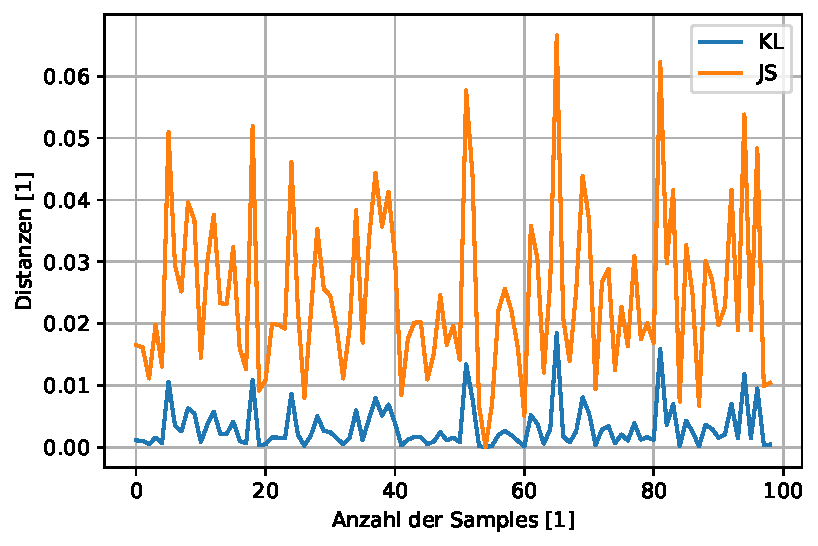
\includegraphics{fig/haupt/math/KL_JS}
	\caption{Vergleich der Kullback-Leibler und Jensen-Shannon Divergence �ber 99 Samples}
	\label{img:math:shannon}
\end{figure}

Es ist zu erkennen, dass der Verlauf der beiden Evaluierungstechniken sehr �hnlich ist. Die Jensen-Shannon Divergence ist hierbei st�rker skaliert, als die Kullback-Leibler Divergence.

\FloatBarrier
\subsection{$\chi^2$-Distance}
\label{sec:haupt:x2}

Eine weitere $f$-Divergence ist die $\chi^2$-Distance. Gem�� \autoref{eqn:tax:fdiv} wird hierbei $f(t) = (t - 1)^2$ verwendet. Daf�r ergibt sich Pearson $\chi^2$ \cite{lit:Cha2007}:
\begin{equation}
	d_{\chi^2}(\mathbb{P},\mathbb{Q}) = \sum\limits_{i = 1}^N \frac{(P_i - Q_i)^2}{Q_i}
	\label{eqn:math:chi2}
\end{equation}
Die \autoref{eqn:math:chi2} kann ebenso in symmetrischer Form auftreten:
\begin{equation}
	d_{\chi^2}(\mathbb{P},\mathbb{Q}) = \sum\limits_{i = 1}^N \frac{(P_i - Q_i)^2}{P_i + Q_i}
	\label{eqn:math:chi2sym}
\end{equation}

\subsection{Hellinger Distance}
\label{sec:haupt:hellinger}

Die Hellinger Distanz geh�rt zu den $f$-Divergences, wenn in \autoref{eqn:tax:fdiv} f�r $f(t) = (\sqrt{t} - 1)^2$ eingesetzt wird. Sie ist nach \autoref{sec:grundl:eval} eine vollwertige Metrik \cite{lit:Gardner2018}. Ebenso ist sie, analog zur Euklidischen Distanz in \autoref{eqn:math:L2}, eine $L_2$-Norm f�r Wahrscheinlichkeitsma�e. Sie ist durch folgende Rechenvorschrift definiert:
\begin{equation}
	d_H(\mathbb{P},\mathbb{Q}) = \sqrt{\sum\limits_{i = 1}^N \left(\sqrt{P_i} - \sqrt{Q_i}\right)^2}
	\label{eqn:math:hellinger}
\end{equation}
\subsection{Mahalanobis Distance}
\label{sec:haupt:mahalanobis}

Die Mahalanobis Distanz geh�rt zu der Klasse der Bregman-Divergences. Hierbei wird in \autoref{eqn:tax:bregman} f�r $\varphi(t) = \frac{1}{2}xAx^T$ eingesetzt. Sie ist definiert durch \cite{lit:Weller2015}:
\begin{equation}
	\parallel x - y \parallel_A = \sqrt{(\det A)^{\frac{1}{n}}(x - y)A^{-1}(x - y)^T}
	\label{eqn:math:mahalanobis}
\end{equation}
In \autoref{eqn:math:mahalanobis}  sind $x$ und $y$ Vektoren, jeweils mit der L�nge $n$. Die Matrix $A$ ist �blicherweise die Kovarianzmatrix. Eine wichtige Eigenschaft ist, dass sie skalen- und translationsinvariant ist.
\subsection{Itakura-Saito Distance}
\label{sec:haupt:itakurasaito}

Die Itakura-Saito Distanz geh�rt zur Familie der Bregman-Divergenzen. Hierbei wird in \autoref{eqn:tax:bregmandiskret} f�r $\varphi(t) = -\log(t)$ eingesetzt \cite{lit:Munoz2015}. Dadurch ergibt sich:
\begin{equation}
	d_\varphi(\mathbb{P},\mathbb{Q}) = \sum\limits_{i = 1}^N \left(\frac{p_i}{q_i} - \log\left(\frac{p_i}{q_i}\right) - 1\right)
	\label{eqn:math:itakura}
\end{equation}

\subsection{Structural Similarity Index}
\label{sec:haupt:ssi}

Der Structural Similarity Index ist, im Normalfall, eine Ma�zahl, die Aussagen �ber die �hnlichkeit zweier Bilder trifft. Es wurde gezeigt, dass diese ebenso f�r vektorielle bzw. sequenzielle Datens�tze $x$ und $y$, mit gleicher L�nge, verwendet werden kann \cite{lit:Parthasarathy2020}. Die folgenden Definitionen, in Bezug auf den Structural Similarity Index, basieren auf \cite{lit:Wang2004}. Die formale Beschreibung eines �hnlichkeitsma� ist definiert durch:
\begin{equation}
	S(x,y) = f\left(l(x,y),c(x,y),s(x,y)\right)
	\label{eqn:math:sim}
\end{equation}
Hierbei wird die �hnlichkeit in drei Komponenten aufgeteilt, die relativ unabh�ngig voneinander sind. $S(x,y)$ ist symmetrisch und auf $\left[0,1\right]$ beschr�nkt. Der Fall $S(x,y) = 1$ liegt nur im Fall $x=y$ vor, \dah wenn die zwei Datens�tze identisch sind. Im Kontext der Bildverarbeitung beschreibt in \autoref{eqn:math:sim} $l(x,y)$ den Lumineszenz-Vergleich, $c(x,y)$ den Kontrast-Vergleich und $s(x,y)$ den Struktur-Vergleich zweier Bilder.

Der Lumineszenz-Vergleich ist abh�ngig von den Mittelwerten $\mu_x$ und $\mu_y$ der entsprechenden Datens�tze:
\begin{equation}
	l(x,y) = \frac{2\mu_x\mu_y + C_1}{\mu_x^2 + \mu_y^2 + C_1}
	\label{eqn:math:siml}
\end{equation}
In \autoref{eqn:math:siml} dient die Konstante zur Stabilisierung des Nenners, falls $\mu_x^2 + \mu_y^2$ sehr nahe an null ist. Eine M�glichkeit w�re die Wahl zu $C_1 = (K_1L)^2$. Hierbei ist $L$ die Spannweite der m�glichen Werte. Im Falle von Pixel-Werten betr�gt diese f�r 8-bit Graustufenbilder 255. $K_1$ ist eine sehr kleine Konstante $K_1 \ll 1$. 

Der Kontrast-Vergleich $c(x,y)$ ist �hnlich beschrieben wie $l(x,y)$, basiert allerdings auf den Standardabweichungen $\sigma_x$ und $\sigma_y$ der entsprechenden Datens�tze:
\begin{equation}
	c(x,y) = \frac{2\sigma_x\sigma_y + C_2}{\sigma_x^2 + \sigma_y^2 + C_2}
	\label{eqn:math:simc}
\end{equation}
�hnlich wie in \autoref{eqn:math:siml} dient die Konstante $C_2$ zur Stabilisierung und kann durch $C_2 = \left(K_2L\right)^2$, mit $K_2 \ll 1$, bestimmt werden.

Analog zum Lumineszenz- und Kontrast-Vergleich kann der Struktur-Vergleich $s(x,y)$ beschrieben werden. Dieser bezieht die Korrelation $\sigma_{xy}$ als Strukturfaktor mit ein:
\begin{equation}
	s(x,y) = \frac{\sigma_{xy} + C_3}{\mu_x^2 + \sigma_y + C_3}
	\label{eqn:math:sims}
\end{equation}

Wenn $l(x,y)$, $c(x,y)$ und $s(x,y)$ zusammengefasst werden, l�sst sich der Structural Similarity Index formal, wie folgt, definieren:
\begin{equation}
	S(x,y) = \left[l(x,y)\right]^\alpha \cdotp \left[c(x,y)\right]^\beta \cdotp \left[s(x,y)\right]^\gamma
	\label{eqn:math:ssim}
\end{equation}
In \autoref{eqn:math:ssim} gilt $\alpha,\ \beta,\ \gamma > 0$. Diese Parameter k�nnen dazu verwendet werden, um die einzelnen Komponenten zu gewichten.

F�r $\alpha = \beta = \gamma = 1$ (gleiche Gewichtung) sowie $C_3 = \frac{C_2}{2}$, ergibt sich folgende Form des Structural Similarity Index:
\begin{equation}
	SSIM(x,y) = \frac{(2\mu_x\mu_y + C_1)(2\sigma_{xy} + C_2)}{(\mu_x^2 + \mu_y^2 + C_1)(\sigma_x^2 + \sigma_y^2 + C_2)}
	\label{eqn:math:ssim1}
\end{equation}
Es ist anzumerken, dass \autoref{eqn:math:ssim1} ausschlie�lich von statistischen Kennzahlen der Datens�tze $x$ und $y$ abh�ngig ist und dementsprechend eine Art von Similarity Coefficient darstellt.

\subsection{Dynamic Time Warping}
\label{sec:haupt:dtw}

Beim Dynamic Time Warping Algorithmus werden zwei Zeitreihen $T = \left\lbrace t_1, t_2, \ldots, t_n \right\rbrace$ und $S = \left\lbrace s_1, s_2, \ldots, s_m \right\rbrace$, unabh�ngig ihrer L�ngen $n$ und $m$, miteinander verglichen \cite{lit:Cassisi2012}. Hierbei liegt der Fokus auf der �hnlichkeit ihrer Formen und nicht auf dem Zeitpunkt ihres Datenpunktes. Dadurch kann, trotz beispielsweise m�glicher Verschiebungen, �hnliche Formen der beiden Datens�tze, erkannt werden. Der Dynamic Time Warp kann ebenso auf allgemeine vektorielle Datens�tze, wie beispielsweise zwei diskrete Dichtefunktionen $\mathbb{P}$ und $\mathbb{Q}$, angewandt werden \cite{lit:Parthasarathy2020}.

Zu Beginn wird die $m \times n$ - Distanzmatrix aufgestellt, welche die Distanzen $d(\mathbb{P}_i, \mathbb{Q}_j)$ (vgl. \autoref{eqn:math:dtwd}) beinhaltet.
\begin{equation}
	distMatrix = \begin{pmatrix}
		d(P_1,Q_1) & d(P_1,Q_2) & \cdots & d(P_1,Q,m) \\
		d(P_2,Q_1) & d(P_2,Q_2) & & \vdots \\
		\vdots & & \ddots & \\
		d(P_n,Q_1) & \cdots & & d(P_n,Q_m)
	\end{pmatrix}
	\label{eqn:math:dtwdist}
\end{equation}
Hierbei entspricht $d(P_i,Q_j)$ der Distanz zwischen den Punkten $P_i$ und $Q_i$ mit $1 \leq i \leq n$ und $1 \leq j \leq m$. Ziel des DTW ist es, den k�rzesten \textit{Warping Path} $W = \left\lbrace w_1, w_2, \ldots, w_K \right\rbrace$, mit $\max(n,m) < K < m + n - 1$ und $w_k = distMatrix(i,j)$, zu finden. F�r die einzelnen $w_k$ bzw. Distanzen in der Distanzmatrix, lassen sich beliebige Distanzfunktionen $d(\cdotp,\cdotp)$ verwenden. Eine solche Distanzfunktion kann \zB, wie folgt beschrieben, definiert werden:
\begin{equation}
	w(\mathbb{P},\mathbb{Q}) = \sum\limits_{i,j}\left(P_i - Q_j\right)^2
	\label{eqn:math:dtwd}	
\end{equation}

Der Algorithmus beginnt bei $w_1 = (1,1)$ und endet maximal bei $w_K = (n,m)$. In jedem Schritt wird, innerhalb der Distanzmatrix, die geringste Distanz aller anliegenden Punkte als n�chstes $w_k$ bestimmt, so dass der \textit{Warping Path} $W$, wie in \autoref{eqn:math:dtwmin} beschrieben, minimiert wird.

\begin{equation}
	DTW(\mathbb{P},\mathbb{Q}) = \min\sqrt{\sum\limits_{k = 1}^{K}  w_k}
	\label{eqn:math:dtwmin}	
\end{equation}
F�r die einzelnen Distanzen $w_k = (i,j)$ bzw. $w_{k - 1} = (i',j')$, mit $i,i' \leq n$ und $j,j' \leq m$, muss gelten:
\newpage
\begin{itemize}
	\item $w_1 = (1,1)\ \wedge \ w_K = (n,m)$
	\item $i - i' \leq 1\ \wedge \ j - j' \leq 1$
	\item $i - i' \geq 0 \ \wedge \ j - j' \geq 0$
\end{itemize}
\section{Gegen�berstellung der Evaluierungstechniken}
\label{sec:haupt:eval}

Im weiteren Verlauf werden die in \autoref{sec:haupt:math} beschriebenen Evaluierungstechniken, anhand ausgew�hlter Bewertungskriterien, bewertet. Nach einer Gegen�berstellung erfolgt die Empfehlung einer Evaluierungstechnik sowie deren Implementierung. Anschlie�end wird diese auf ausgew�hlte generierte Daten angewandt und die Ergebnisse validiert.

\subsection{Bewertung der Evaluierungstechniken}
\label{sec:haupt:bewert}
Im Folgenden werden die in \autoref{sec:haupt:math} beschriebenen Evaluierungstechniken, auf Basis von ausgew�hlten Bewertungskriterien, qualitativ bewertet. Die hierbei verwendeten Kriterien werden nachfolgend genannt und beschrieben.

\begin{description}
	\item[Effektivit�t (E)] Die Effektivit�t einer Evaluierungstechnik ist stellvertretend f�r die Qualit�t bzw. G�te des zugrundeliegenden �hnlichkeitsma�es. Im zugrundeliegenden Anwendungsfall kann diese als wichtigstes Kriterium betrachtet werden. Die G�te ist dabei, teils stark, von den entsprechenden Daten abh�ngig. Ein weiterer Aspekt von hoher Relevanz ist die Entwicklung bzw. der Verlauf der �hnlichkeitswerte. Diese sollten plausible Werte �ber den gesamten Wertebereich liefern.
	\item[Komplexit�t (K)] Zur Komplexit�t der Evaluierungstechniken geh�rt die Zeitkomplexit�t. Diese kann anhand der jeweiligen Implementierung bestimmt werden. Hierbei wird die Big-O Notation - oder auch Landau Symbol $\mathcal{O}$ - verwendet. Daraus folgt ebenso die entsprechende Laufzeit bzw. Effizienz der Evaluierungstechnik. Diese ist von der Anzahl an Datenpunkten abh�ngig.
	\item[Anwendbarkeit (A)] Die Anwendbarkeit einer Evaluierungstechnik ist davon abh�ngig, wie einfach diese auf eine Wahrscheinlichkeitsdichtefunktion anwendbar ist. Es ist hierbei zu beachten, ob die zugrundeliegende Implementierung mit einem hohen Aufwand verbunden ist. Beispielsweise in Form von Optimierungsprozessen.
	\item[Transparenz (T)] Die Transparenz ist ein Ma� f�r die Klarheit und den Umfang der Evaluierungstechnik. Insbesondere ob gen�gend Literaturquellen diese Methode fundiert und ausf�hrlich beschreiben.
	\item[Robustheit (R)] Die Robustheit einer Evaluierungstechnik beschreibt, inwiefern diese mit Messungenauigkeiten umgehen kann. Hierzu z�hlen beispielsweise Peaks, Rauschen oder Ausrei�er der Daten.
	\item[Parametrisierbarkeit (P)] Die Parametrisierbarkeit gibt an, ob die Evaluierungstechnik Parameter enth�lt und falls dieses der Fall ist, inwiefern diese, nach Qualit�tsaspekten, einzustellen sind. Beispielsweise existieren Parameter, die typischerweise �ber Optimierungsprozesse oder empirische Methoden bestimmt werden.
	\item[Interpretierbarkeit (I)] Die Interpretierbarkeit gibt an, wie gut die Daten bzw. Ergebnisse der Evaluierungstechnik interpretiert werden k�nnen. Methoden, die standardisiert, auf einen Wertebereich beschr�nkt sind oder gegen einen bestimmten Wert konvergieren, haben hierbei eine hohe Aussagekraft. Falls dies nicht der Fall ist, k�nnen die Ergebnisse, auf Basis von Expertenwissen oder Erfahrungswerten, qualitativ bewertet bzw. interpretiert werden.
\end{description}

Nachfolgend werden die genannten Bewertungskriterien in drei verschiedene Stufen eingeteilt. Die beschriebenen Kriterien k�nnen, anhand der Symbole \enquote{+} als positive, \enquote{o} als neutrale sowie \enquote{-} als negative Eigenschaft, auftreten. Ein genauere Beschreibung der Unterteilung erfolgt in \autoref{tab:haupt:krit}.

\begin{table}[h!]
	\centering
	\begin{tabular}{l|c|p{0.69\linewidth}}
		\toprule
		Effektivit�t & + & Evaluierungstechnik wei�t eine hohe Qualit�t auf.\\
		\midrule
		& o & Evaluierungstechnik wei�t eine m��ige Qualit�t auf.\\
		\midrule
		& - & Evaluierungstechnik wei�t eine niedrige Qualit�t auf.\\
		\midrule
		Komplexit�t & + & Evaluierungstechnik besitzt eine niedrige Zeitkomplexit�t und Laufzeit.\\
		\midrule
		& o & Evaluierungstechnik besitzt eine m��ige Zeitkomplexit�t und Laufzeit.\\
		\midrule
		& - & Evaluierungstechnik besitzt eine hohe Zeitkomplexit�t und Laufzeit.\\
		\midrule
		Anwendbarkeit & + & Evaluierungstechnik l�sst sich grunds�tzlich leicht umsetzen oder (Referenz-)Implementierung(en) sind vorhanden.\\
		\midrule
		& o & Evaluierungstechnik l�sst sich nur bedingt einfach umsetzen. Es stehen keine (Referenz-)Implementierungen zur Verf�gung.\\
		\midrule
		& - & Evaluierungstechnik l�sst sich grundlegend schwierig umsetzen und
		(Referenz-)Implementierungen stehen nicht zur Verf�gung.\\
		\midrule
		Transparenz & + & Evaluierungstechnik ist transparent beschrieben und verst�ndlich.\\
		\midrule
		& o & Evaluierungstechnik ist eher m��ig transparent beschrieben (\zB mathematische
		Beschreibung nicht vollst�ndig dokumentiert).\\
		\midrule
		& - & Evaluierungstechnik setzt ein vertieftes mathematisches Wissen
		voraus und/oder dessen Beschreibung ist gr��tenteils unvollst�ndig.\\
		\midrule
		Robustheit & + & Evaluierungstechnik ist robust gegen�ber Ungenauigkeiten der Daten (z. B.
		Messfehler, Rauschen oder Ausrei�er).\\
		\midrule
		& o & Die Evaluierungstechnik ist nicht vollkommen robust gegen�ber Ungenauigkeiten
		der Daten.\\
		\midrule
		& - & Die Evaluierungstechnik ist nicht robust gegen�ber Ungenauigkeiten der Daten.\\
		\midrule
		Parametrisierbarkeit & + & Die Evaluierungstechnik beinhaltet keine oder nur wenige Parameter. Falls diese Parameter umfasst, dann sind sie leicht einstellbar.\\
		\midrule
		& o & Die Evaluierungstechnik beinhaltet mehrere Parameter. Diese sind nicht alle einfach einstellbar.\\
		\midrule
		& - & Die Evaluierungstechnik beinhaltet mehrere bis viele Parameter. Zumindest die meisten davon sind nicht einfach einstellbar.\\
		%Evaluierungstechnik wei�t eine hohe Parametrisierbarkeit auf. F�r die Ermittlung dieser ist ein hoher Aufwand oder ein Optimierungsprozess notwendig. keine und kein anwendungsfall\\
		\midrule
		Interpretierbarkeit & + & Das Ergebnis der Evaluierungstechnik ist leicht interpretierbar.\\
		\midrule
		& o & Das Ergebnis der Evaluierungstechnik ist m��ig interpretierbar.\\
		\midrule
		& - & Das Ergebnis der Evaluierungstechnik l�sst sich schwierig interpretieren.\\
		\bottomrule
	\end{tabular}
	\caption{Beschreibung der Bewertungskriterien}
	\label{tab:haupt:krit}
\end{table}

Weiterhin erfolgt eine Gegen�berstellung der Evaluierungstechniken, auf Basis der beschriebenen Bewertungskriterien, in \autoref{tab:haupt:eval}.

\begin{table}[h]
	\centering
	\begin{tabular}{p{0.35\linewidth}|P{0.05\linewidth}|P{0.09\linewidth}|P{0.05\linewidth}|P{0.05\linewidth}|P{0.05\linewidth}|P{0.05\linewidth}|P{0.05\linewidth}}
		\toprule
		\textbf{Evaluierungstechnik} & \textbf{E} & \textbf{K} & \textbf{A} & \textbf{T} & \textbf{R} & \textbf{P} & \textbf{I} \\
		\midrule
		Kolmogorov-Smirnov & + & + $\mathcal{O}(n)$ & o & + & - & - & +\\
		\midrule
		Wasserstein & + & \cellcolor{cyan!50} & o & o & \cellcolor{orange!50} & - & \cellcolor{orange!50}\\
		\midrule
		Cram�r & o & + $\mathcal{O}(n)$ & o & + & o & + & +\\
		\midrule
		Minkowski & o & + $\mathcal{O}(n)$ & + & + & o & o & +\\
		\midrule
		Maximum Mean Discrepancy & o & \cellcolor{cyan!50} & o & o & + & - & \cellcolor{cyan!50}\\
		\midrule
		Total Variation Metric & + & + $\mathcal{O}(n)$ & + & + & o & + & +\\
		\midrule
		Kullback-Leibler & + & + $\mathcal{O}(n)$ & + & + & + & + & +\\
		\midrule
		Jensen-Shannon & + & + $\mathcal{O}(n)$ & + & + & + & + & +\\
		\midrule
		$\chi^2$ & + & + $\mathcal{O}(n)$ & + & + & - & + & o\\
		\midrule
		Hellinger & + & + $\mathcal{O}(n)$ & + & + & o & + & +\\
		\midrule
		Mahalanobis & o & + & + & + & + & o & o\\
		\midrule
		Itakura-Saito & + & + $\mathcal{O}(n)$ & + & o & o & + & o\\
		\midrule
		Structural Similarity Index & o & + & + & + & o & o & +\\
		\midrule
		Dynamic Time Warping & + & o $\mathcal{O}(n^2)$& + & o & + & o & o\\
		\bottomrule
	\end{tabular}
	\caption{Bewertung der Evaluierungstechniken}
	\label{tab:haupt:eval}
\end{table}

\FloatBarrier
Die beiden Farben in \autoref{tab:haupt:eval} haben die folgende Bedeutung:

\begin{itemize}
	\item Cyan: Das Kriterium kann, aufgrund der mathematischen Beschreibung der zugrundeliegenden Evaluierungstechnik, nicht zweckdienlich eingestuft werden.
	\item Orange: Das Kriterium (zugeh�rig zur jeweiligen Evaluierungstechnik) kann, aufgrund begrenzter Literatur, nicht zweckdienlich eingestuft werden.
\end{itemize}

Die Implementierung der Kolmogorov-Smirnov Distanz erfolgt, wie in \autoref{eqn:math:ksdiskret} beschrieben, durch die simple Ermittlung der maximalen Differenz zweier kumulativer Verteilungsfunktionen. Diese muss jedoch zun�chst, f�r die �bergebenen Wahrscheinlichkeitsdichtefunktionen, iterativ berechnet werden.
\\
\\
Die Wasserstein-1 Distanz - oder auch Earth Mover's Distance - beschreibt die \enquote{Kosten}, um eine Wahrscheinlichkeitsdichtefunktion, mit Hilfe einer Transformation,  in eine andere zu �berf�hren. Hierbei wird die statistische Geometrie der Dichtefunktionen ber�cksichtigt. Daraus folgt eine hohe Qualit�t der hieraus resultierenden Diskrepanzen. Die Eigenschaften der Wasserstein Distanz sind stark abh�ngig von der gew�hlten Transformation. Daraus folgt eine hohe Parametrisierbarkeit, mit der Folge, dass die Wahl dieser in einem Optimierungsproblem resultiert. Es lassen sich hierbei keine allgemeinen Aussagen �ber die entsprechende Komplexit�t der Transformation treffen. Diese bestimmt ebenso die Anwendbarkeit bzw. wie leicht sie zu implementieren ist. Zudem bestimmt diese die Robustheit gegen�ber etwaigen Messungenauigkeiten.
\\
\\
Die Cram�r Distanz entspricht der quadrierten Differenz von kumulativen Verteilungsfunktionen. Dementsprechend muss diese, in der Implementierung, iterativ berechnet werden.
\\
\\
Die Minkowski Metrik ist eine verallgemeinerte Evaluierungstechnik, die verschiedene Distanzen beinhaltet. Die Werte sind hierbei nicht normalisiert und m�ssen, in einem weiteren Schritt, qualitativ bewertet werden. Im Allgemeinen besitzen die entsprechenden Distanzen, da es sich um Metriken handelt (vgl. \autoref{sec:grundl:eval}), eine hohe Qualit�t. In \autoref{eqn:math:minkowskidiskret} sind die Spezialf�lle, durch die Wahl des Parameters $p$, bestimmt. Ein gr��eres $p$ bewirkt hierbei eine h�here Gewichtung der gr��ten Differenz zweier Wahrscheinlichkeitsdichtefunktionen. Somit kann die Robustheit gegen�ber Messungenauigkeiten, wie beispielsweise Ausrei�ern, angepasst werden. Die Wahl eines passenden Wertes f�r $p$ stellt allerdings einen Optimierungsprozess dar.
\\
\\
Die Maximum Mean Discrepancy ist, wie viele andere Integral Probability Metrics, durch eine hohe Parametrisierbarkeit gekennzeichnet. Sie ist durch die Wahl einer reproduzierenden Kernelfunktion definiert. Die Zeitkomplexit�t ist hierbei von dem gew�hlten Kernel abh�ngig. Dieser bestimmt ebenso die Anwendbarkeit. Es handelt sich um eine komplexe Evaluierungstechnik, die ein vertieftes Verst�ndnis in der Mengenlehre, speziell in Bezug auf den reproduzierenden Kernel Hilbertraum, voraussetzt. Die Kernelfunktion besitzt, auf Basis ihrer Definition, einen Gl�ttungseffekt, wodurch sich eine hohe Robustheit gegen�ber Messungenauigkeiten ergibt.
\\
\\
Die Total Variation Metric ist auf [0,1] beschr�nkt und verf�gt dementsprechend �ber eine hohe Aussagekraft. Sie kann als $f$-Divergence sowie als Integral Probability Metric beschrieben werden.
\newpage
Die Kullback-Leibler Divergence ist ein Ma� der relativen Entropie und besitzt eine hohe Qualit�t. Um diese Divergence besser nachvollziehen zu k�nnen, ist ein grundlegendes Wissen �ber informationstheoretische Ma�e, speziell die Entropie, vorauszusetzen. Dennoch ist sie leicht zu implementieren. Durch ihre Skaleninvarianz ist sie Robust gegen�ber Ausrei�ern. Sie ist Parameter-unabh�ngig. Da es sich hierbei um ein Divergenzma� handelt, sind die Ergebnisse leicht zu interpretieren. Umso n�her das Ergebnis bei null liegt, desto �hnlicher sind sich die �bergebenen Wahrscheinlichkeitsdichtefunktionen. Bei identischen Dichtefunktionen ergibt sich f�r die Kullback-Leibler Divergence ein Wert von null.
\\
\\
Die Jensen-Shannon Divergence ist eine symmetrische Version der Kullback-Leibler Divergence. Folglich besitzt sie �hnliche Eigenschaften. Die Evaluierungstechnik weist ebenfalls eine hohe Qualit�t auf. Sie ist robust gegen�ber Messungenauigkeiten, leicht verst�ndlich und leicht zu implementieren. Das Ergebnis l�sst, sich analog zur Kullback-Leibler Divergence, interpretieren.
\\
\\
Die $\chi^2$-Distance kann in symmetrischer oder asymmetrischer Form beschrieben werden. In beiden F�llen ist sie leicht verst�ndlich und implementierbar.
\\
\\
Die Hellinger Distanz ist eine vollwertige Metrik und auf [0,1] beschr�nkt. Aufgrund der metrischen Eigenschaften, besitzt sie eine hohe G�te. Werte, die n�her bei null liegen, weisen hierbei auf �hnliche Wahrscheinlichkeitsdichtefunktionen. Folglich l�sst sie sich leicht interpretieren.
\\
\\
Die Mahalanobis Distanz ist eine Bregman-Divergence und nicht normalisiert bzw. auf einen bestimmten Wertebereich beschr�nkt. Umso n�her ein Wert bei null liegt, desto �hnlicher sind sich die �bergebenen Datens�tze. Das Ergebnis muss folglich qualitativ bewertet werden. Sie besitzt den Parameter $A$, der meistens als die Kovarianzmatrix gew�hlt wird. Durch ihre Skalen- und Translationsinvarianz ist sie robust gegen�ber Messungenauigkeiten. Es wird ein grundlegendes Verst�ndnis der linearen Algebra und Statistik ben�tigt, um sie zu verstehen. Dennoch ist die Implementierung leicht durchzuf�hren.
\\
\\
Die Itakura-Saito Distanz erfordert, um sie zu verstehen, ein vertieftes Wissen �ber Divergenzma�e, speziell �ber die Bregman-Divergences. Sie ist dennoch leicht anzuwenden.
\\
\\
Der Structural Similarity Index ist auf [0,1] beschr�nkt. Hierbei ergibt sich, f�r den Fall von identischen Datens�tzen, ein Wert von eins. F�r den Fall, dass die Datens�tze sich f�r keinen Punkt �hneln, ergibt sich ein Wert gegen null. Folglich l�sst sich das Ergebnis leicht interpretieren. Da nur verschiedene statistische Kennzahlen miteinander verrechnet werden, wei�t dieses �hnlichkeitsma� eine begrenzte Qualit�t auf. Die Evaluierungstechnik ist durch eine hohe Parametrisierbarkeit charakterisiert. Diese m�ssen, in einem Optimierungsprozess, bestimmt werden. Es handelt sich um ein sehr spezielles �hnlichkeitsma� aus der Bildverarbeitung, zu dem nicht viel Literatur zur Verf�gung steht.
\\
\\
Der Dynamic Time Warping Algorithmus ist nicht normalisiert oder auf einen bestimmten Wertebereich beschr�nkt. Ein Ergebnis, dass nah bei null liegt, wei�t auf eine hohe �hnlichkeit der Wahrscheinlichkeitsdichtefunktionen. Da es sich allerdings um kein Divergenzma� handelt, muss das Ergebnis noch qualitativ bewertet werden. Der Algorithmus verwendet eine weitere Methode der Distanzberechnung. Dadurch ergibt sich eine hohe Parametrisierbarkeit. Es muss dementsprechend, vor der Implementierung, eine passende Methode bestimmt werden. \\Ebenso ist der Algorithmus robust gegen�ber Messungenauigkeiten. Der Grund hierf�r liegt, unter anderem, in der Translationsinvarianz dieser Methode. Zudem wird, bei der Berechnung, die statistische Geometrie der Dichtefunktionen miteinbezogen. Hierdurch ergibt sich eine hohe Qualit�t.
\\
\\
Anhand der in \autoref{tab:haupt:eval} durchgef�hrten Bewertung und Gegen�berstellung der Evaluierungstechniken, ergeben sich drei �u�erst relevante Methoden. Diese sind namentlich die Kullback-Leibler und Jensen-Shannon Divergence sowie die Hellinger Distance. Jeder dieser Evaluierungstechniken wei�t, in Bezug auf die genannten Bewertungskriterien, ausschlie�lich positive Einstufungen auf. Bei einer solchen Gleichheit (Patt-Situation) ist es eine bew�hrte Methode, eine Endauswahl, auf Basis der Literaturnennungen, im (angrenzenden) Anwendungsfall, zu treffen. Dies trifft auf die Kullback-Leibler Divergenz zu. Aus diesem Grund wird die Kullback-Leibler Divergenz, als entsprechende Evaluierungstechnik, empfohlen.

\FloatBarrier
\subsection{Implementierung}
\label{sec:haupt:valid}

Die Evaluierung von generativen Algorithmen, unter Verwendung der Wahrscheinlichkeitsdichtefunktionen, erfolgt mit Hilfe der in \autoref{sec:haupt:bewert} empfohlenen Kullback-Leibler Divergenz. Hierzu wird die Evaluierungstechnik implementiert. Die Komplettumsetzung bzw. Pipeline der angrenzenden Doktorarbeit verwendet die Programmiersprache Python \cite{lit:Schick2021}. Aus diesem Grund wird diese ebenso f�r die Implementierung verwendet. Python umfasst hierbei eine Vielzahl an Package bzw. Bibliotheken, die im Kontext der K�nstlichen Intelligenz und deren Teilgebiete, verwendet werden k�nnen \cite{lit:Raschka2019}\cite{lit:Foster2020}.
Der Funktionsprototyp wird wie folgt definiert:

\begin{itemize}
	\item[] \textbf{[y1, y2, y3] = f(P,Q)}
\end{itemize}

Hierbei werden der Funktion zwei Parameter \textbf{P} und \textbf{Q} �bergeben. Diese entsprechen den Wahrscheinlichkeitsdichtefunktionen. Der R�ckgabewert \textbf{y1} stellt die Kullback-Leibler Divergenz dar. Neben dieser sind ebenso zwei weitere Kennzahlen f�r die eigentliche Validierung vorgesehen. Hierbei wird die Kullback-Leibler Divergenz iterativ berechnet. Die Gr��e \textbf{y2} beschreibt den maximalen Einzelwert der Kullback-Leibler Divergenz zwischen zwei Punkten der beiden Wahrscheinlichkeitsdichtefunktionen (maximale Diskrepanz). Dieser macht Aussagen �ber die h�chste Diskrepanz von zwei Werten der entsprechenden Wahrscheinlichkeitsdichtefunktionen. Die Gr��e \textbf{y3} gibt den maximalen Gradienten der jeweiligen Einzelwerte an. Die zwei R�ckgabewerte \textbf{y2} und \textbf{y3} dienen zur Validierung, inwieweit die beiden Wahrscheinlichkeitsdichtefunktionen in plausiblen Wertebereichen liegen.

Die Implementierung erfolgt in \autoref{lst:haupt:kl}. Hierbei werden in einem ersten Schritt, mit Hilfe der \textit{where} Funktion des NumPy Packages, die Einzelwerte der Kullback-Leibler Divergenz bestimmt. Die Ermittlung der eigentlichen Kullback-Leibler Divergenz erfolgt mit Hilfe der \textit{sum} Funktion. Der maximale Gradient wird durch die Verkettung der \textit{max} und \textit{gradient} Funktionen bestimmt. Abschlie�end werden die drei genannten Kennzahlen zur�ckgegeben. 
\newpage
\begin{lstlisting}[language=Python, caption=Python Code: Kullback-Leibler Divergence, label=lst:haupt:kl]
def kullback_leibler(p,q):
	"""
	
	"""
	# Einzelwerte der Kullback-Leibler Divergenz
	kl_vals = np.where(q != 0, p * np.log(p / q), 0)
	# Kullback-Leibler Divergenz
	kl_div = np.sum(kl_vals)
	# maximaler Einzelwert
	max_val = np.max(kl_vals)
	# maximaler Gradient
	max_gradient = np.max(np.gradient(kl_vals))
	return kl_div, max_val, max_gradient
\end{lstlisting}
\subsection{Datenanalyse}
\label{sec:haupt:data}

Im Folgenden wird die implementierte Kullback-Leibler Divergenz auf verschiedene synthetisch generierte Datens�tze angewandt, mit dem Ziel, die Ergebnisse zu validieren. Hierbei werden zwei F�lle betrachtet. In einem ersten Schritt werden synthetisch generierte Sinusfunktionen, als sogenannte Baseline (Referenz), analysiert. Darauffolgend werden synthetisch generierte �berholvorg�nge betrachtet. In beiden F�llen werden die spezifischen Variationsparameter nur geringf�gig ver�ndert. Dadurch f�llt es leichter, eine qualitative Aussage �ber die generierten Daten zu machen, da diese leichter zu interpretieren sind. Die hierbei verwendeten Wahrscheinlichkeitsdichtefunktionen werden allesamt mittels der Histogramm-Spline-Approximation bestimmt.
\\
\\

\subsubsection*{\textbf{Sinusfunktion}}

In \autoref{img:data:sinFktK} sind 100 synthetisch generierte Sinusfunktionen als Zeitreihe dargestellt. Diese wurden mit Hilfe des Python Codes in \autoref{lst:a:sin} generiert. Es wurden hierbei 1000 Datenpunkte verwendet. Diese sind durch folgende Rechenvorschrift definiert:

\begin{equation}
	f(t) = a ~\cdotp sin(b ~\cdotp (t + c)) + d
	\label{eqn:data:sinFkt}
\end{equation}

Die Variationsparameter $a, b, c$ und $d$ besitzen jeweils eine Abweichung von $ \pm 0,01$ mit einer Schrittweite von $0,001$. Durch diese Variation ergeben sich verschiedene Verl�ufe f�r die Funktionen. In \autoref{img:data:sinFktA} sind diese Varianzen, f�r einen Ausschnitt, genauer dargestellt.

\begin{figure}
	\centering
	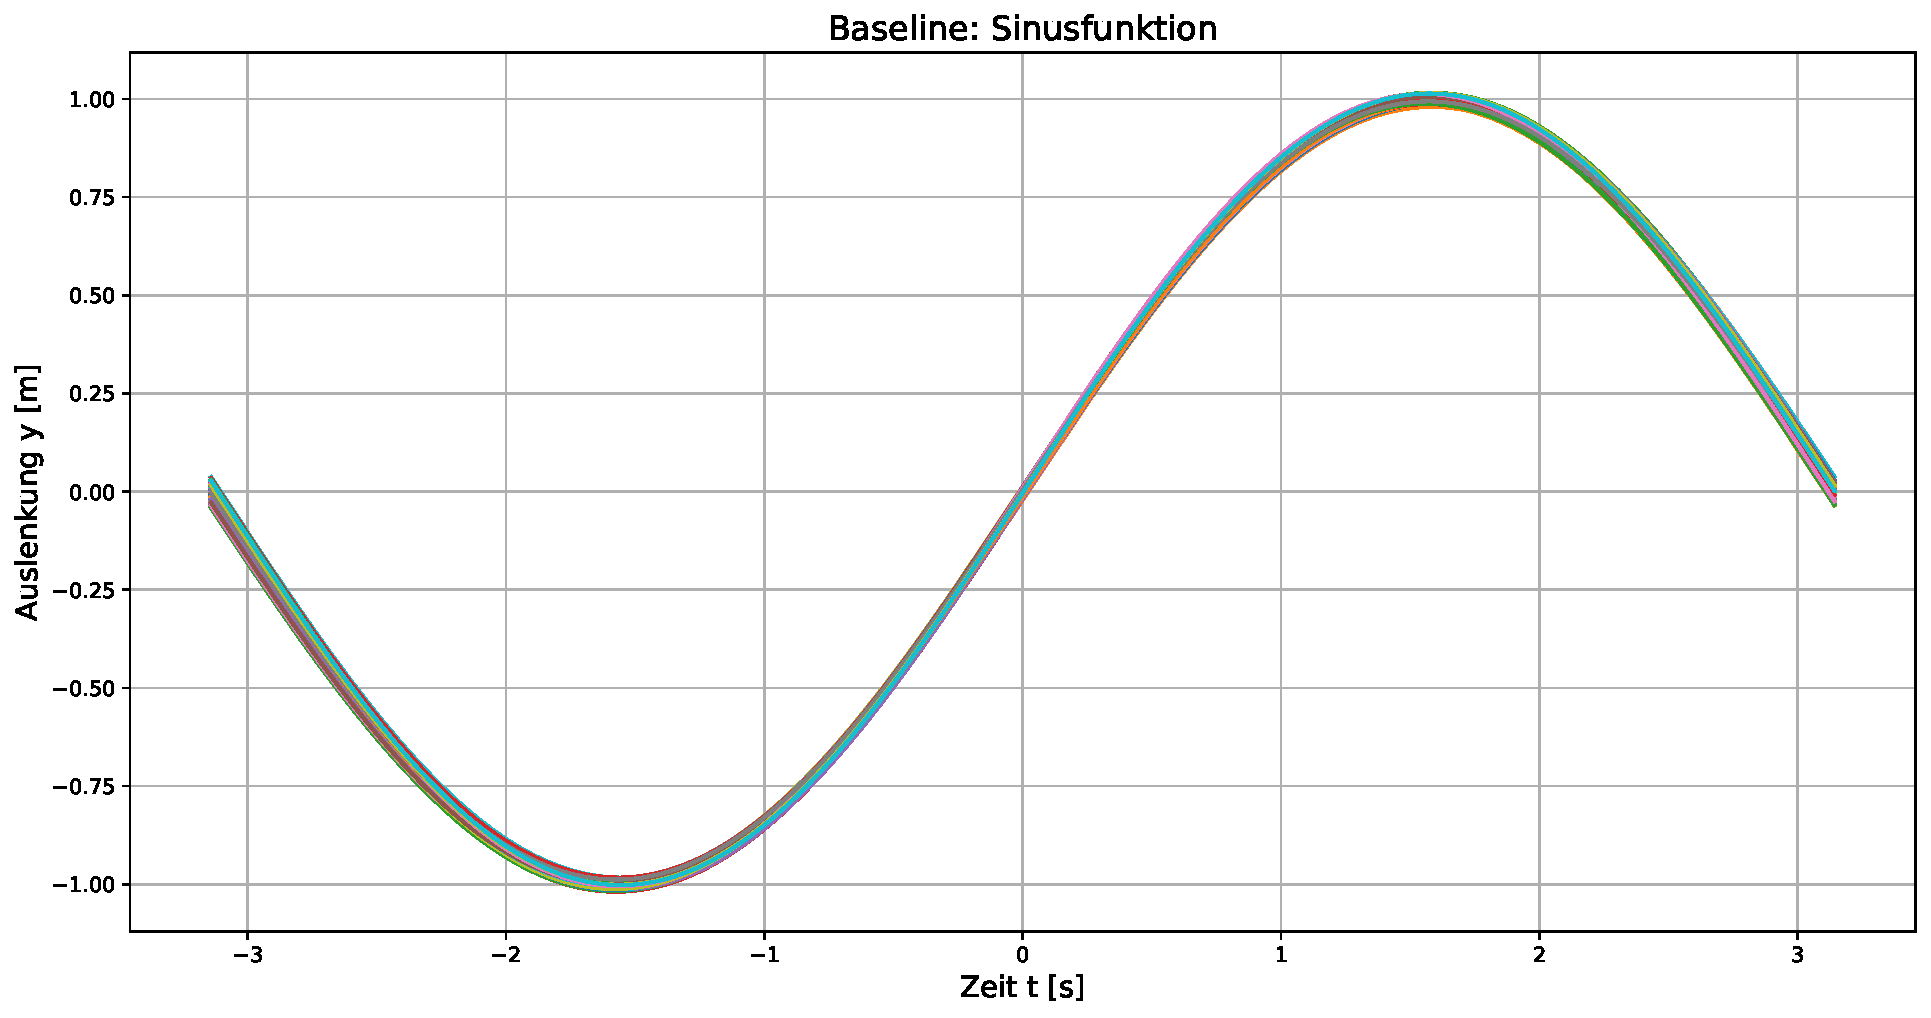
\includegraphics[width=\linewidth,height=0.6\linewidth]{fig/haupt/impl/SinusfunktionKomplett}
	\caption{Sinusfunktionen}
	\label{img:data:sinFktK}
\end{figure}

\begin{figure}
	\centering
	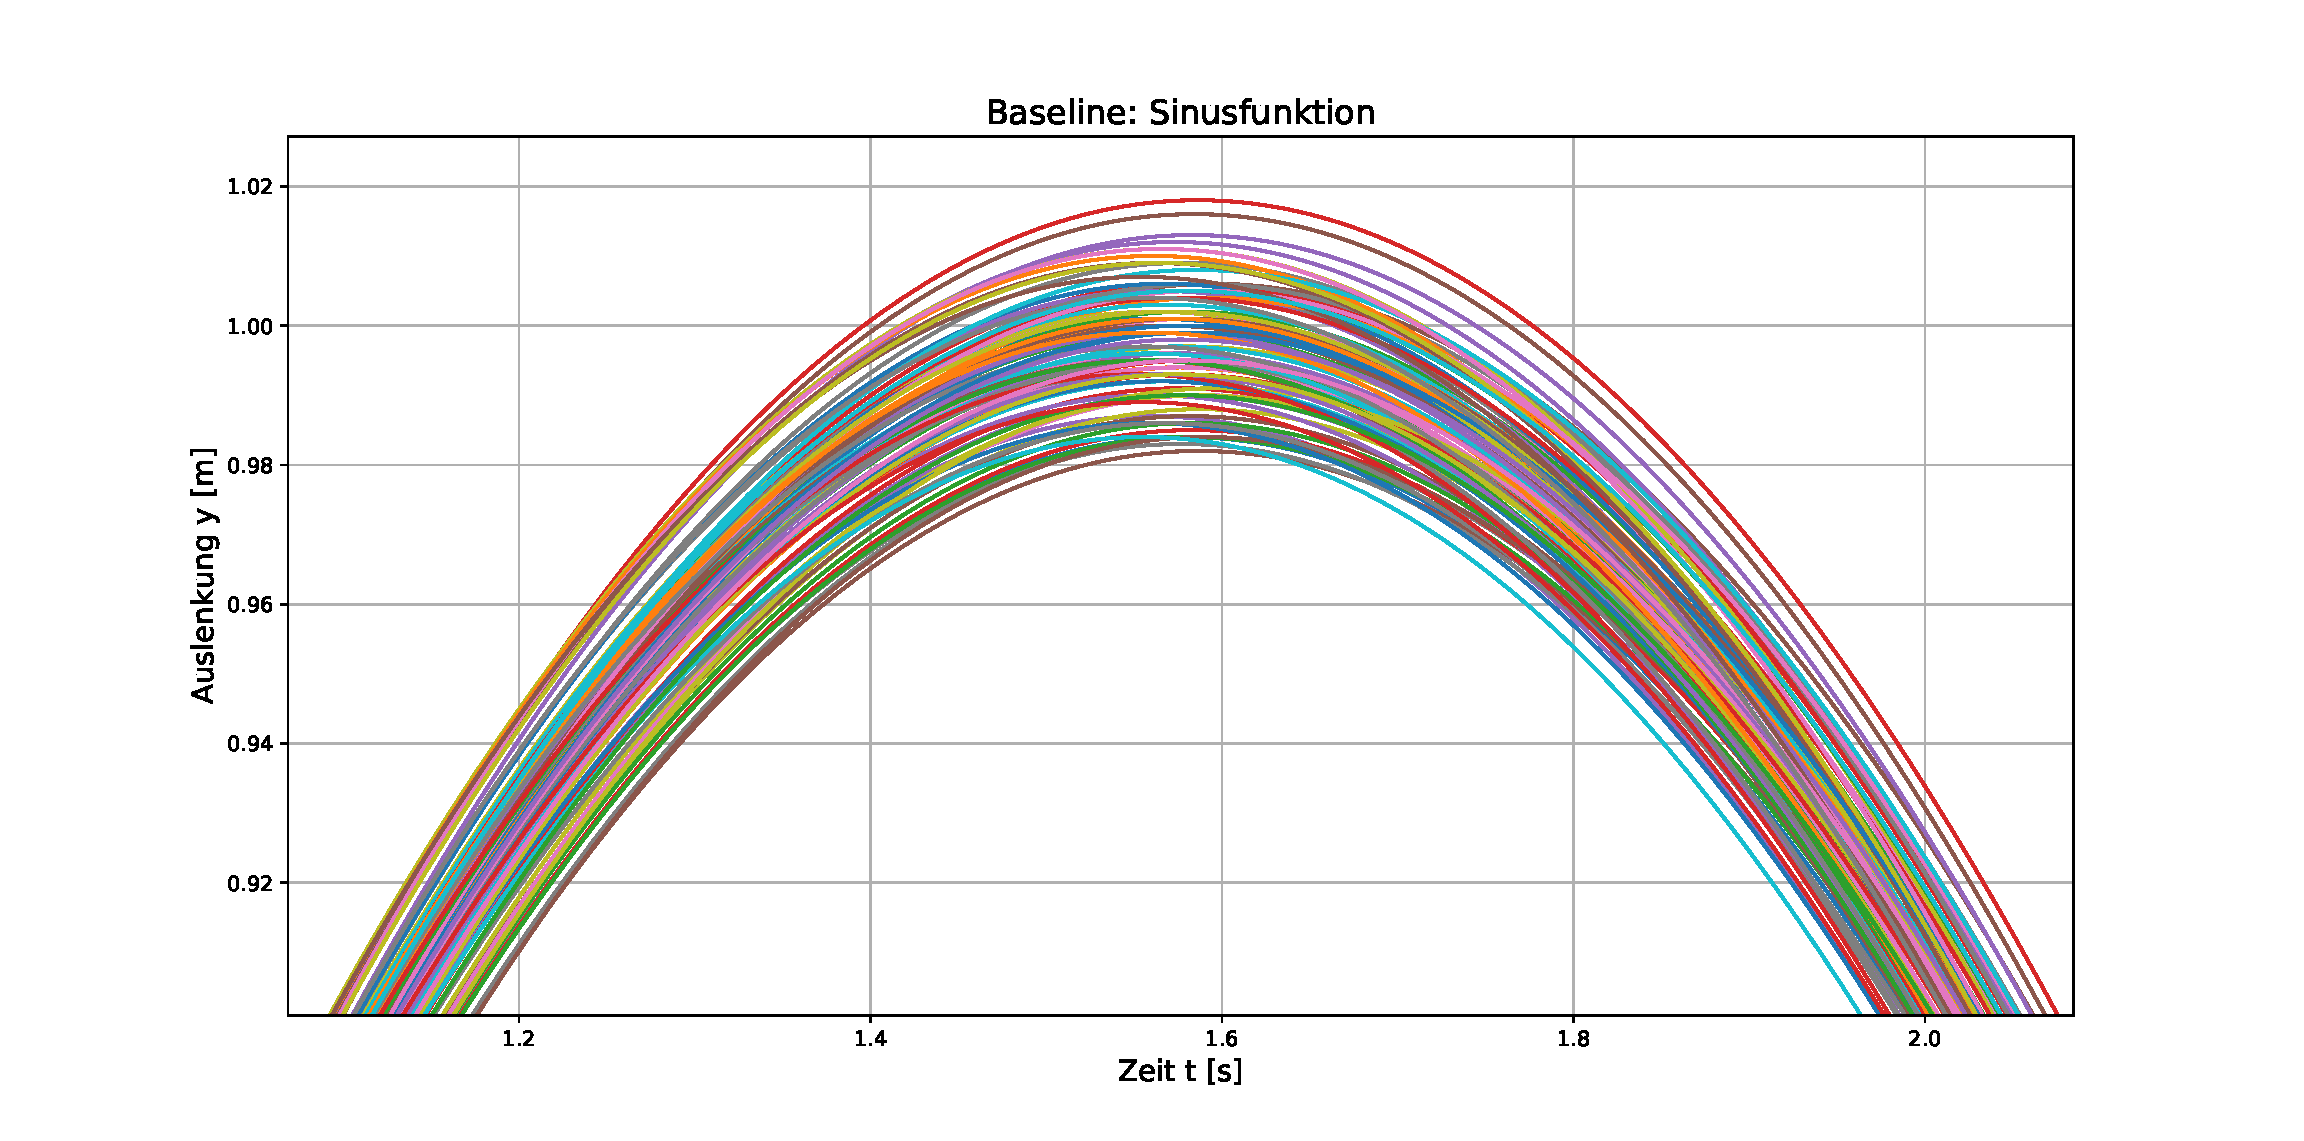
\includegraphics[width=\linewidth,height=0.6\linewidth]{fig/haupt/impl/SinusfunktionAusschnitt}
	\caption{Ausschnitt der Sinusfunktionen}
	\label{img:data:sinFktA}
\end{figure}

Die Wahrscheinlichkeitsdichtefunktionen der Sinusfunktionen sind, in \autoref{img:data:sinDichtK}, �ber der Auslenkung $y$, dargestellt. Die entsprechenden Dichtefunktionen wurden mittels der Histogramm-Spline-Approximation bestimmt (vgl. \autoref{sec:grundl:fkt}). Hierbei wurden sieben Bins f�r das zugrundeliegende Histogramm und ein Ann�herungspolynom 5. Grades verwendet.
\\
\\
In Bezug auf Sinusfunktionen sind hierbei drei Punkte von hoher Relevanz. Diese sind namentlich der Hochpunkt, Tiefpunkt sowie der Nulldurchgang. F�r die Extrempunkte ergeben sich hierbei hohe Varianzen. Da die Steigung um diese Punkte gering ist, �ndert sich die Auslenkung nur schwach. \\Folglich sind f�r diese Auslenkungen die meisten Datenpunkte vorhanden. Dies spiegelt sich ebenso in den Dichtefunktionen in \autoref{img:data:sinDichtK} wieder. Hierbei sind f�r die Auslenkungen $y = \pm 1,00$ die h�chsten relativen Wahrscheinlichkeiten zu verzeichnen. Die Dichtefunktionen weisen hierbei ebenso hohe Varianzen auf.
\\
\\
In den Nulldurchg�ngen besitzen die, in \autoref{img:data:sinFktK} dargestellten Sinusfunktionen, die h�chste Steigung. Folglich �ndert sich die Auslenkung, um diese Stellen, am schnellsten, �ber der Zeit. Hierbei ergeben sich, bei Variation der Parameter, hohe Varianzen. Diese sind ebenso in den Wahrscheinlichkeitsdichtefunktionen in \autoref{img:data:sinDichtK} bzw. \autoref{img:data:sinDichtA} zu verzeichnen. 
\\
\\
F�r die verschiedenen Dichtefunktionen sind einige Punkte mit einer h�heren Konzentration zu beobachten. Dies wird vor allem in \autoref{img:data:sinDichtA}, f�r die Auslenkungen $y \approx \pm 2,5$, deutlich. Der Grund hierf�r liegt in der Histogramm-Spline-Approximation selbst. Hierbei werden Splines durch die Klassenmitten des zugrundeliegenden Histogrammes gelegt. Dadurch ergeben sich ebenso Punkte mit h�herer Konzentration bei den Klassenmitten.

\begin{figure}
	\centering
	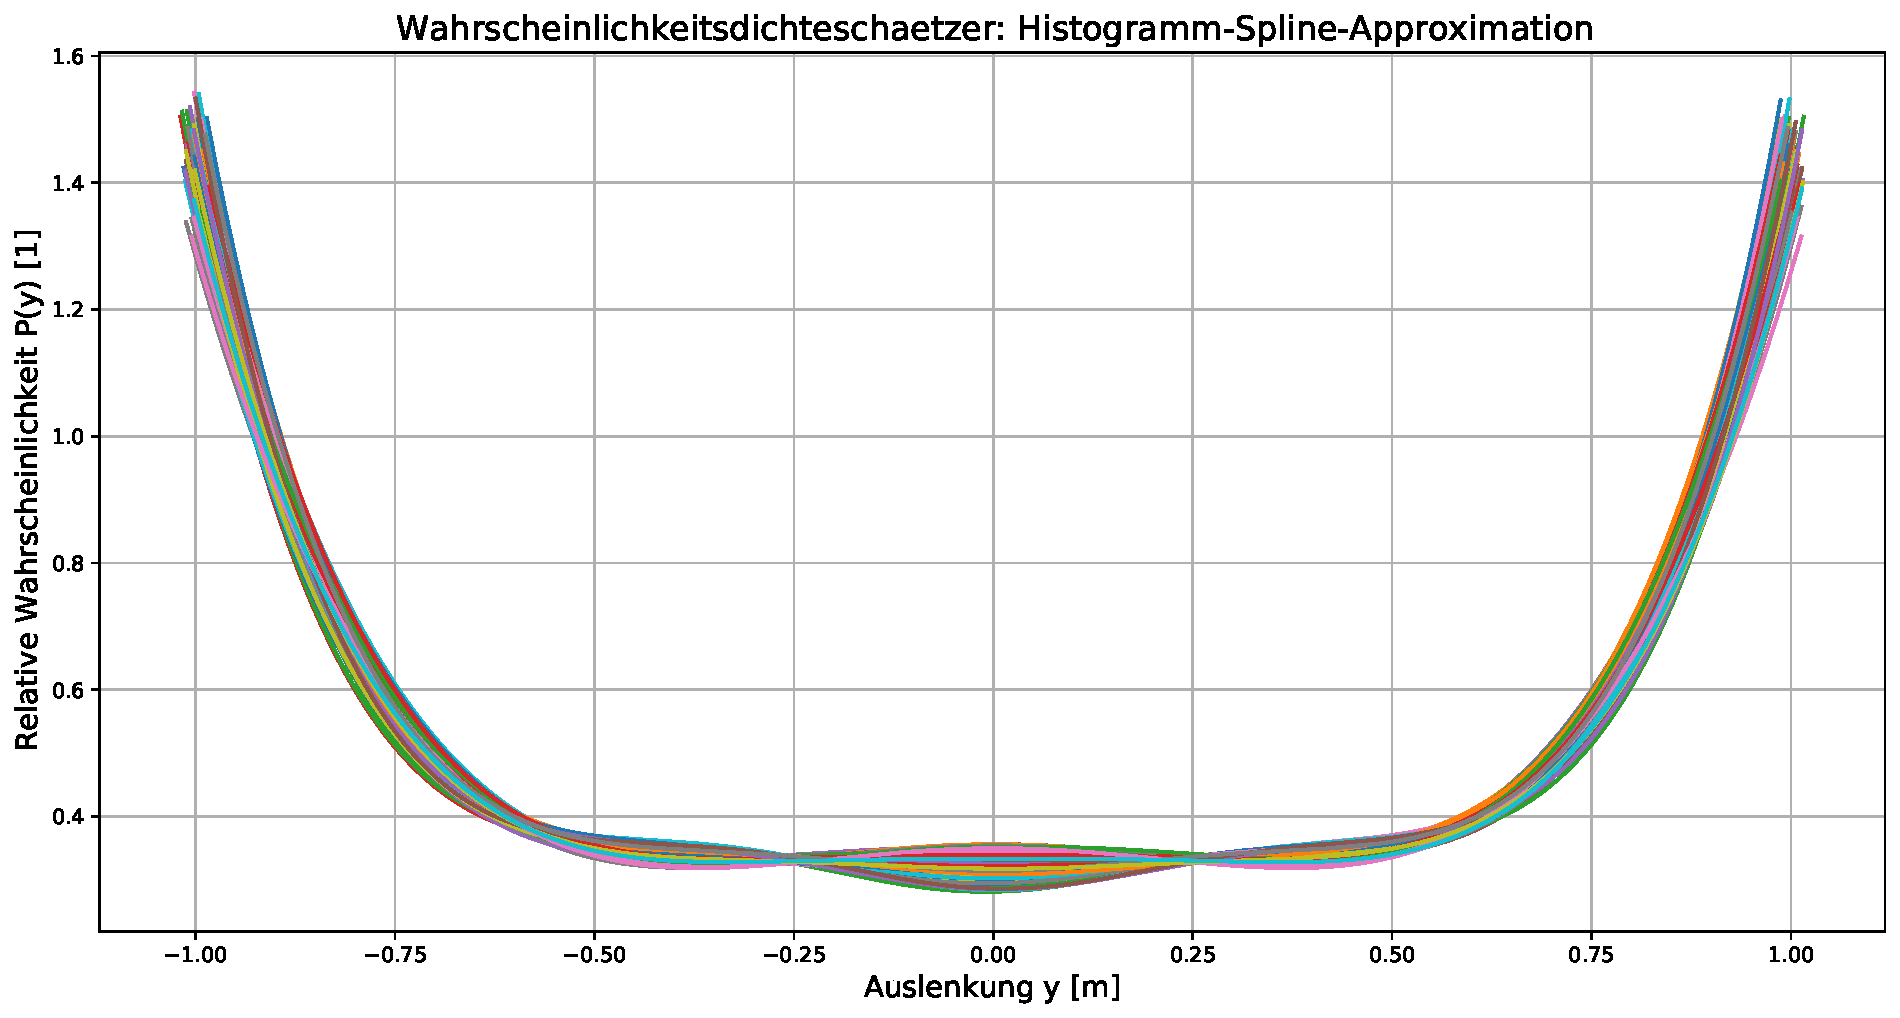
\includegraphics[width=\linewidth,height=0.6\linewidth]{fig/haupt/impl/SinusfunktionDichtefunktionKomplett}
	\caption{Wahrscheinlichkeitsdichtefunktionen von Sinusfunktionen}
	\label{img:data:sinDichtK}
\end{figure}

\begin{figure}
	\centering
	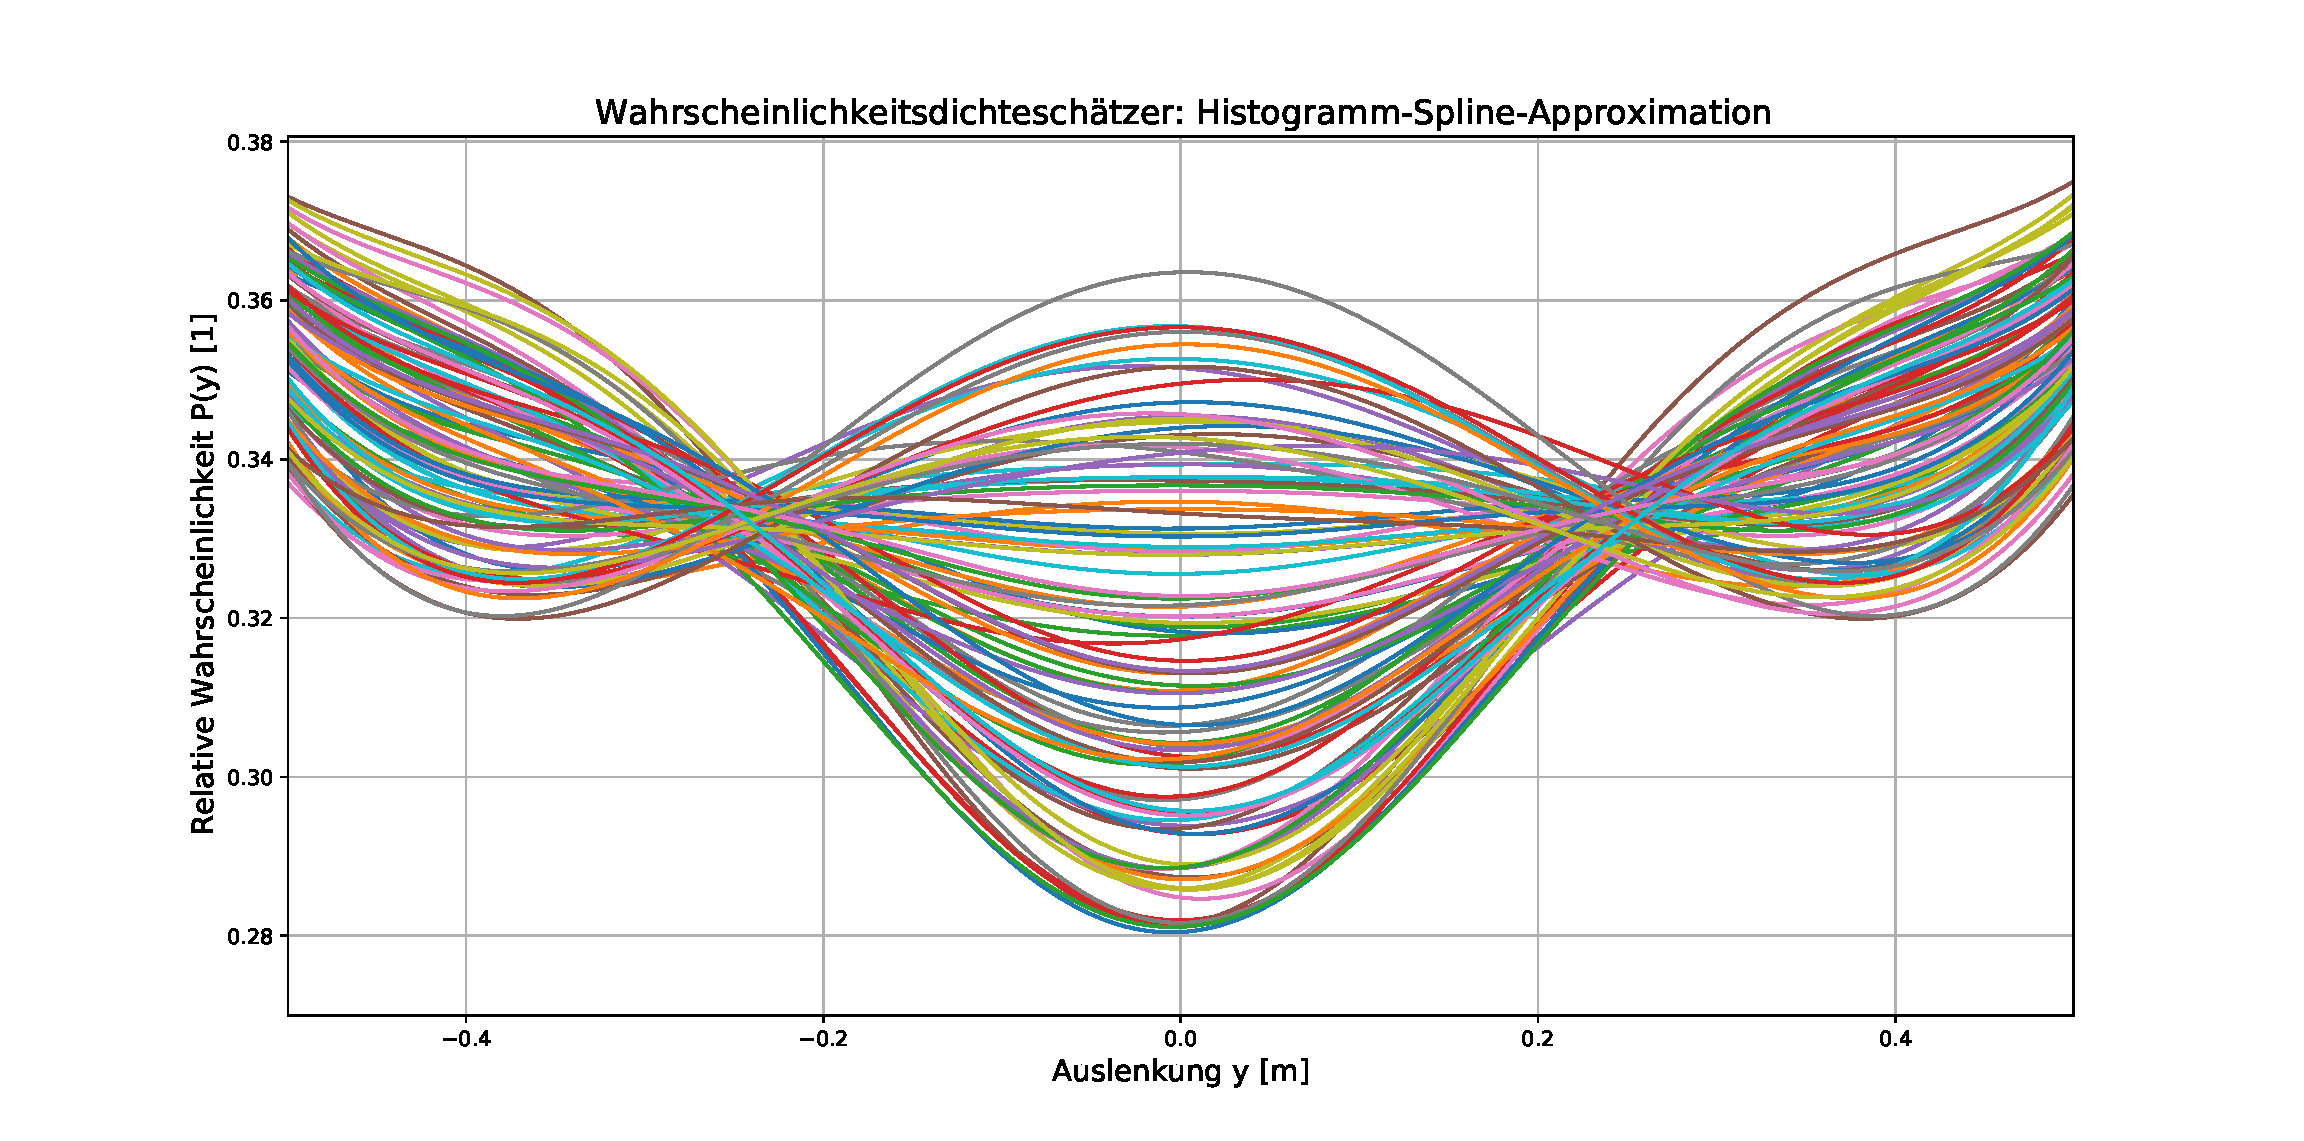
\includegraphics[width=\linewidth,height=0.6\linewidth]{fig/haupt/impl/SinusfunktionDichtefunktionAusschnitt}
	\caption{Ausschnitt der Wahrscheinlichkeitsdichtefunktionen von Sinusfunktionen}
	\label{img:data:sinDichtA}
\end{figure}

In \autoref{img:data:sinKLK} sind die Kullback-Leibler Distanzen f�r die Wahrscheinlichkeitsdichtefunktionen von 99 Sinusfunktionen dargestellt. Eine der 100 Dichtefunktionen wurde hierbei als Referenz-Dichtefunktion verwendet. Es ergeben sich ausschlie�lich Werte nahe null. Dies spricht f�r eine sehr hohe �hnlichkeit der Kurven.
\\
\\
Neben den eigentlichen aufsummierten Kullback-Leibler Divergenzen sind deren Einzelwerte relevant. Durch diese lassen sich die Verl�ufe der Wahrscheinlichkeitsdichtefunktionen validieren. In \autoref{img:data:sinKLA} sind die Einzelwerte f�r 99 Samples dargestellt. \\Es sind die verschiedenen Bereiche mit hoher Varianz zu erkennen, die mit den Varianzen aus \autoref{img:data:sinDichtK} �bereinstimmen. Es sind ebenfalls die sieben Bins des zugrundeliegenden Histogramms zu erkennen, die f�r die Histogramm-Spline-Approximation verwendet werden. Die Grenzen dieser Histogramme liegen an den Stellen mit einer h�heren Konzentration.

\begin{figure}
	\centering
	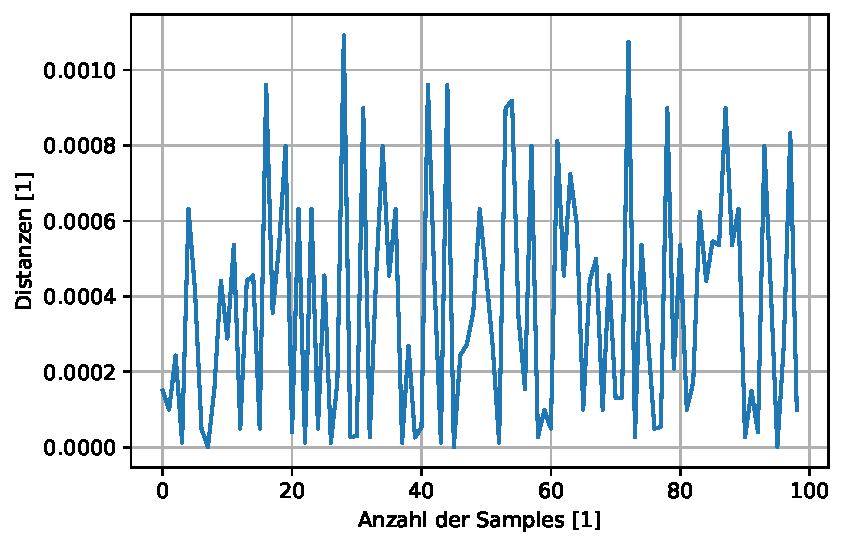
\includegraphics[width=\linewidth,height=0.6\linewidth]{fig/haupt/impl/SinKLK}
	\caption{Kullback-Leibler Distanzen f�r Dichtefunktionen der Sinusfunktionen}
	\label{img:data:sinKLK}
\end{figure}

\begin{figure}
	\centering
	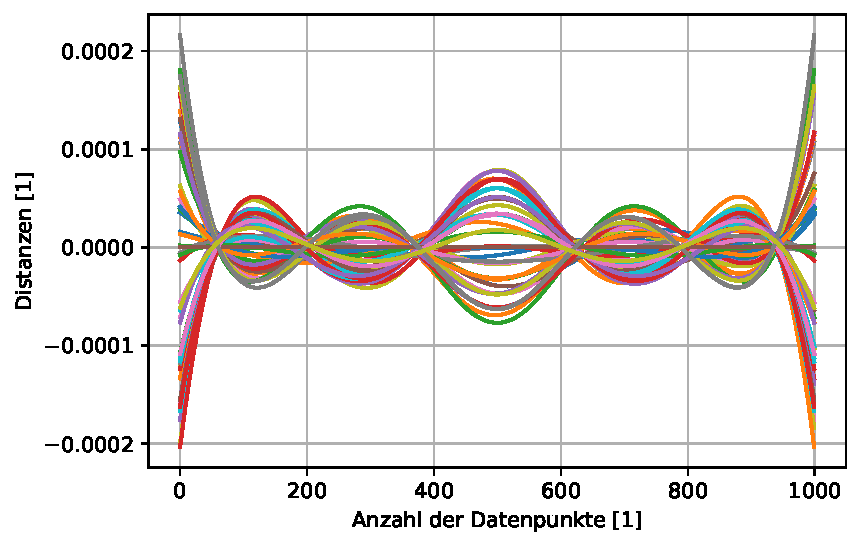
\includegraphics[width=\linewidth,height=0.6\linewidth]{fig/haupt/impl/SinKLEinzel}
	\caption{Einzelwerte der Kullback-Leibler Distanzen f�r Dichtefunktionen der Sinusfunktionen}
	\label{img:data:sinKLA}
\end{figure}

\FloatBarrier

\subsubsection*{\textbf{�berholvorgang}}

Nachfolgend werden synthetisch generierte �berholvorg�nge, vergleichbar mit denen in \autoref{img:haupt:ueberhol}, analysiert. Die dazugeh�rigen Bewegungsdaten sind in \autoref{img:data:ueberFktK} als Zeitreihen, f�r die L�ngs- und Querrichtung, dargestellt. Diese wurden mit Hilfe des Python Codes in \autoref{lst:a:ueber} generiert. Es wurden hierbei 1602 Datenpunkte verwendet.
\\
\\
Die entsprechenden Verl�ufe basieren auf den kinematischen bzw. physikalischen Beschreibungen in \cite{lit:Schick2020}. Hierbei besitzen die Variationsparameter $\gamma_1$ und $\gamma_2$ jeweils eine Abweichung von $ \pm 0,1$ mit einer Schrittweite von $0,001$. Durch diese Variation der Parameter ergeben sich unterschiedliche Bewegungsverl�ufe des �berholenden Fahrzeugs.
\\
\\
Es sind deutliche Varianzen in den Bewegungsverl�ufen f�r die Ein- und Ausschervorg�nge zu erkennen. In \autoref{img:data:ueberFktA} sind diese beispielhaft f�r den Ausschervorgang dargestellt. Im Gegensatz dazu sind, w�hrend des �berholvorgangs auf der Gegenfahrbahn, die Variation der einzelnen Verl�ufe gering.

\begin{figure}
	\centering
	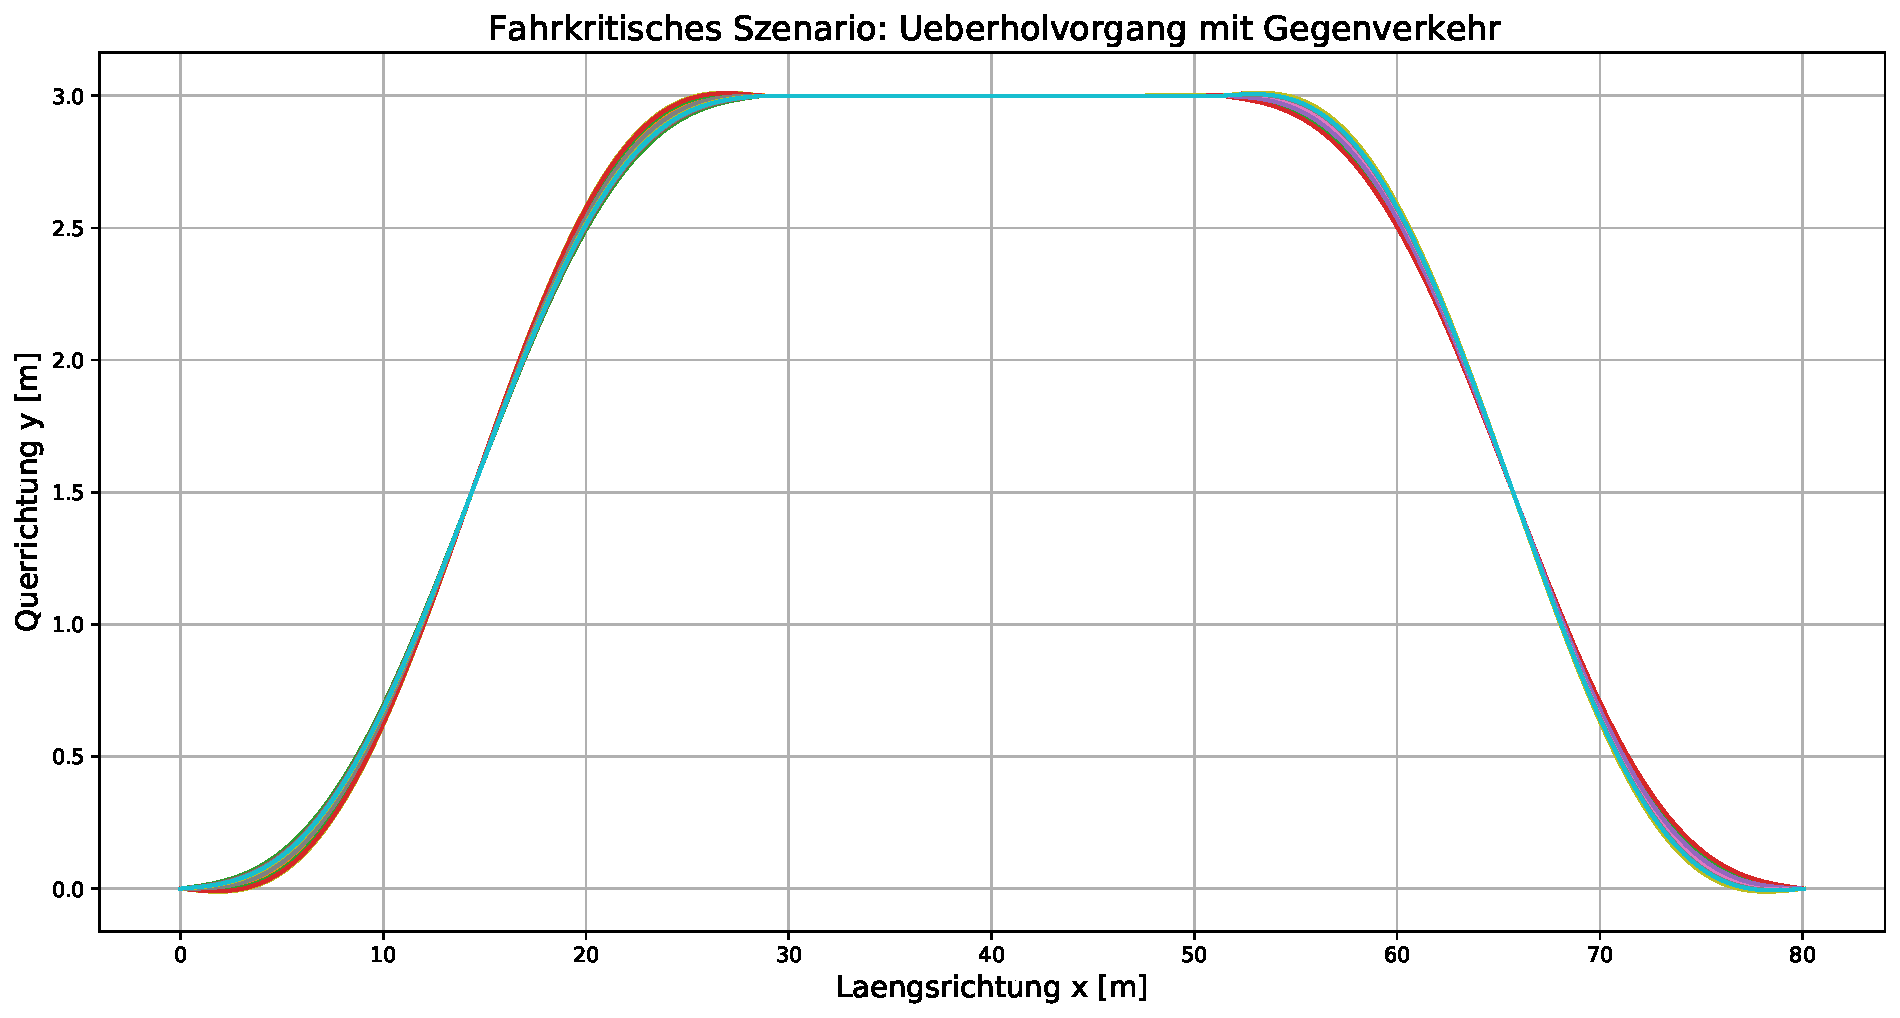
\includegraphics[width=\linewidth,height=0.6\linewidth]{fig/haupt/impl/UeberholvorgangFunktionKomplett}
	\caption{Bewegungsdaten von synthetisch generierten �berholvorg�ngen}
	\label{img:data:ueberFktK}
\end{figure}

\begin{figure}
	\centering
	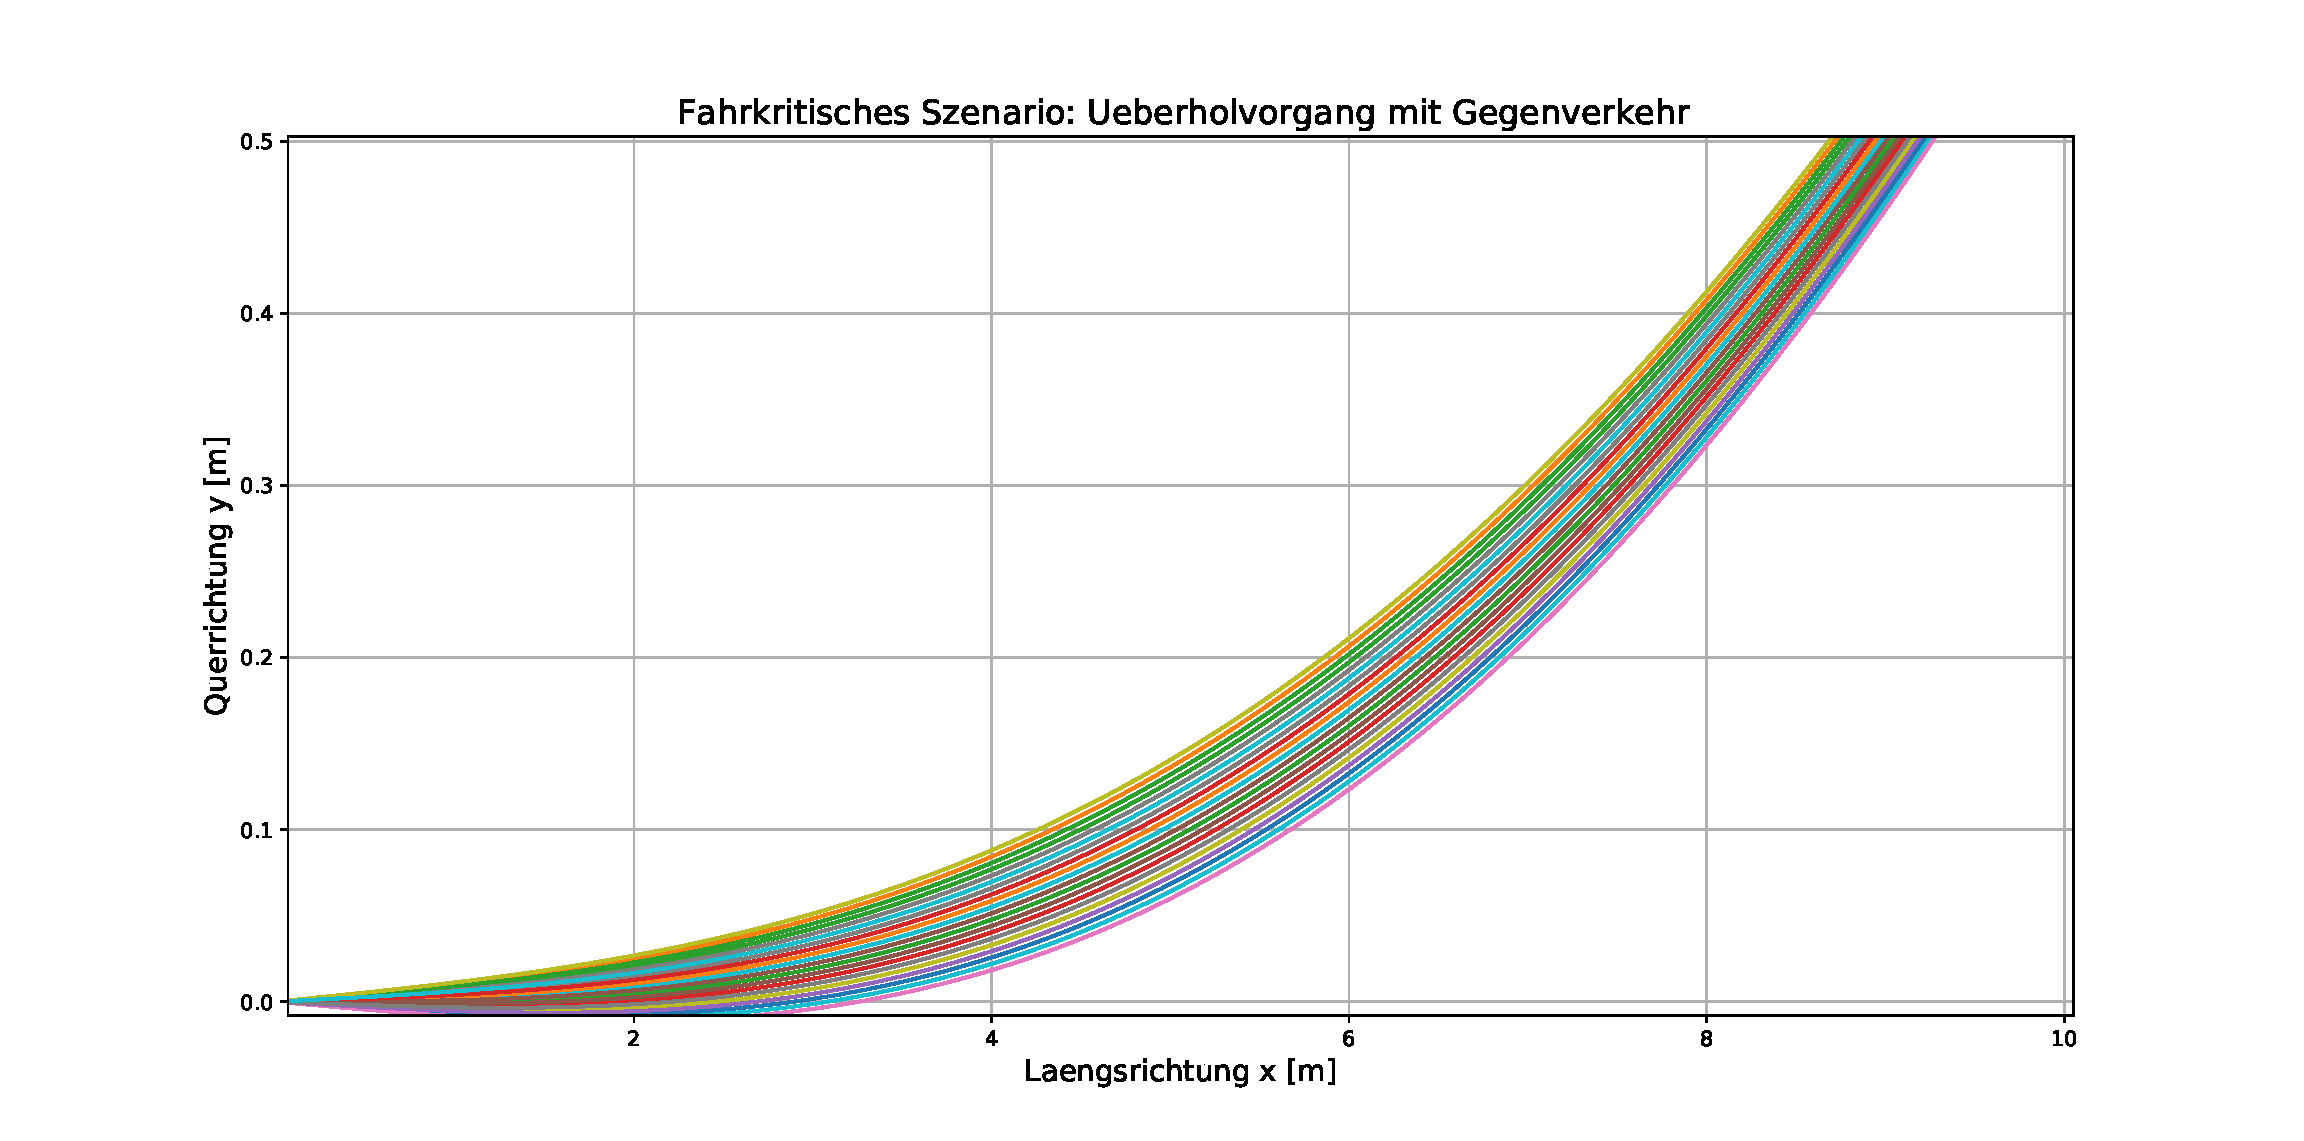
\includegraphics[width=\linewidth,height=0.6\linewidth]{fig/haupt/impl/UeberholvorgangFunktionAusschnitt}
	\caption{Ausschnitt der Bewegungsdaten von synthetisch generierten �berholvorg�ngen}
	\label{img:data:ueberFktA}
\end{figure}

In \autoref{img:data:ueberDichtK} sind die Wahrscheinlichkeitsdichtefunktionen �ber der Querrichtung dargestellt. Diese wurden ebenso mit Hilfe der Histogramm-Spline-Approximation bestimmt. Hierbei wurden 13 Bins f�r das zugrundeliegende Histogramm und ein Ann�herungspolynom 11. Grades verwendet. Insgesamt werden die Variationen der einzelnen Wahrscheinlichkeitsdichtefunktionen deutlich. Diese ergeben sich durch die unterschiedlichen Bewegungsverl�ufe.
\\
\\
F�r eine Querrichtung nahe null befindet sich das Fahrzeug auf der urspr�nglichen Fahrbahn. Hierbei ergeben sich relativ hohe Werte f�r die relative Wahrscheinlichkeit. Ebenso sind hohe Varianzen zu beobachten, die aus den unterschiedlichen Bewegungsverl�ufen resultieren. F�r eine Querrichtung nahe drei befindet sich das Fahrzeug auf der Gegenfahrbahn. Hierbei sind, aufgrund der geringen Variation in den Bewegungsverl�ufen w�hrend des �berholvorgangs, die h�chsten relativen Wahrscheinlichkeiten zu verzeichnen. Die Dauer des Ein- und Ausschervorgangs ist, relativ zum �berholvorgang, gering. Aus diesem Grund ergibt sich, f�r eine Auslenkung in Querrichtung von $0,5$ bis $2,5$ m, eine relative Wahrscheinlichkeit nahe null.
\\
\\
In \autoref{img:data:ueberDichtA} ist ein Ausschnitt der Dichtefunktionen �ber der Querrichtung, zugeh�rig zur �berholspur des �berholvorgangs auf der Gegenfahrbahn, dargestellt. Die Variationen der einzelnen Bewegungsverl�ufe sind auf dieser gering. Dadurch sind die relativen Wahrscheinlichkeiten dort entsprechend gr��er. Die Variationen der einzelnen Wahrscheinlichkeitsdichtefunktionen werden hierbei wiederum verdeutlicht. Der Grund hierf�r liegt in den unterschiedlichen Phasen der Ein- und Ausschervorg�ngen.

\begin{figure}
	\centering
	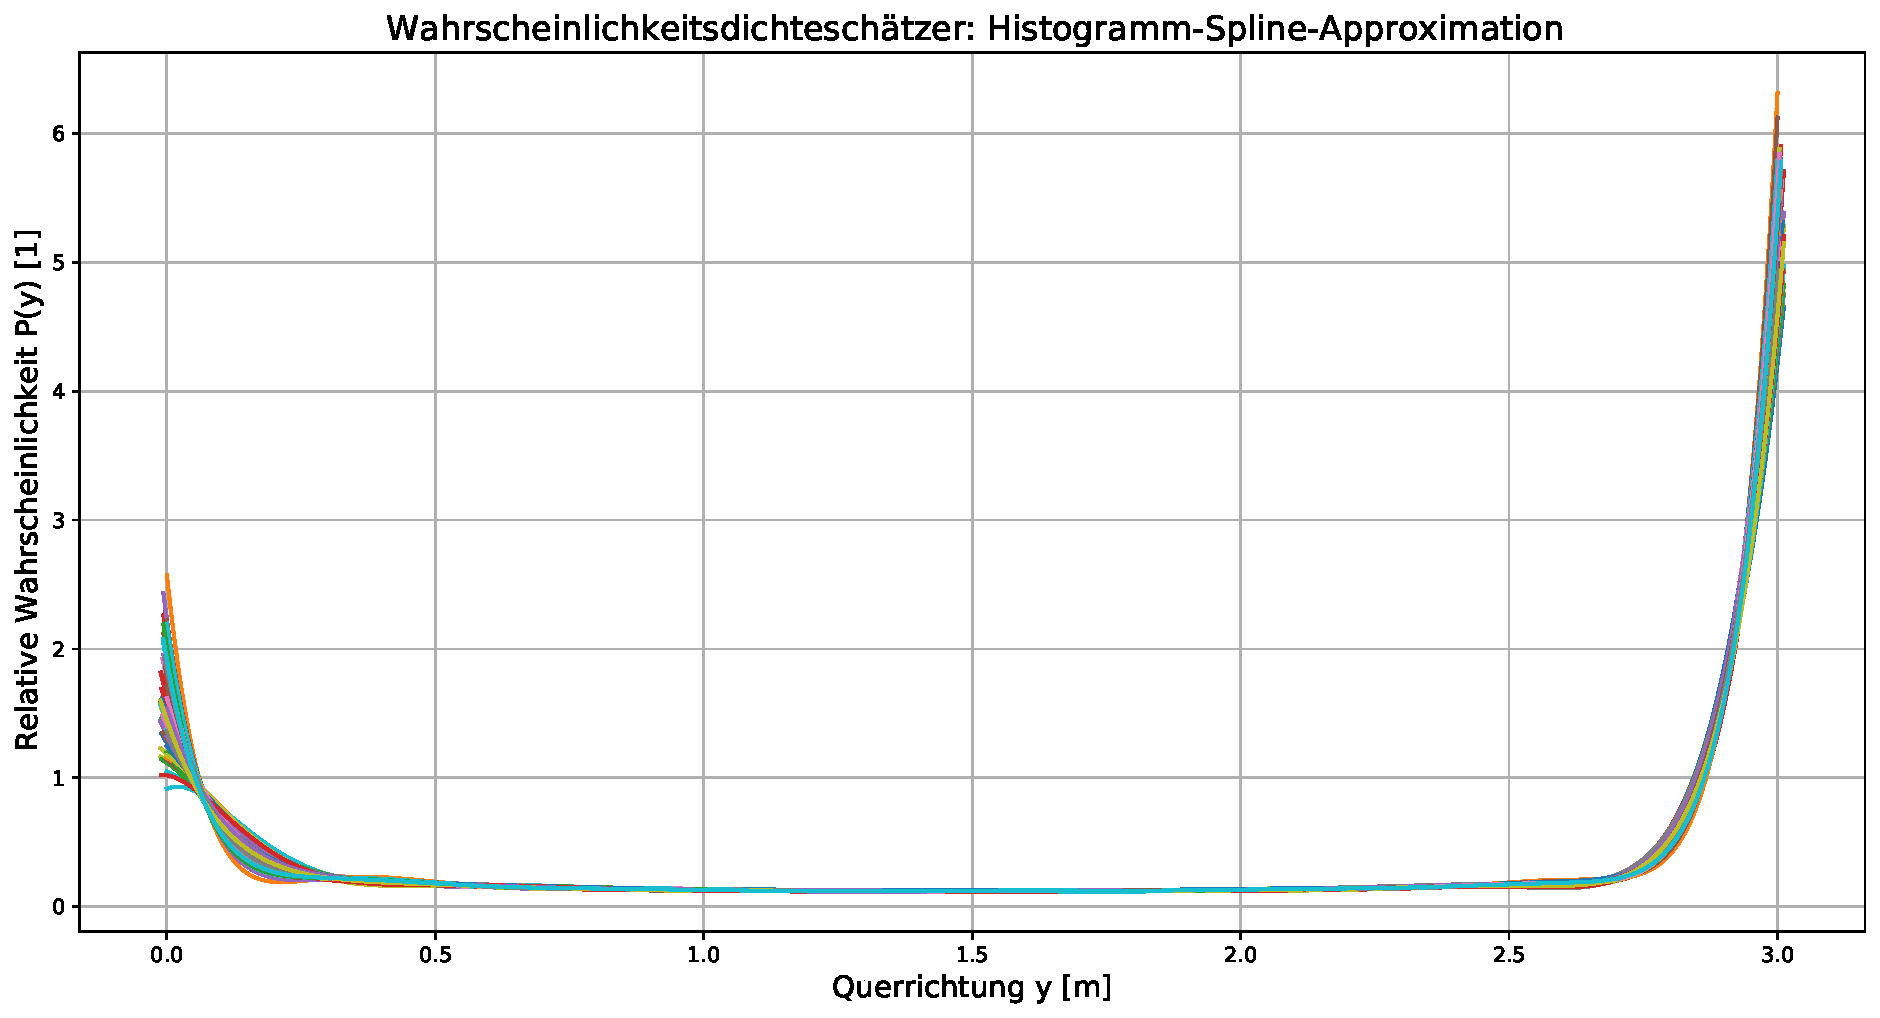
\includegraphics[width=\linewidth,height=0.6\linewidth]{fig/haupt/impl/UeberholvorgangDichtefunktionKomplett}
	\caption{Dichtefunktionen von synthetisch generierten �berholvorg�ngen}
	\label{img:data:ueberDichtK}
\end{figure}

\begin{figure}
	\centering
	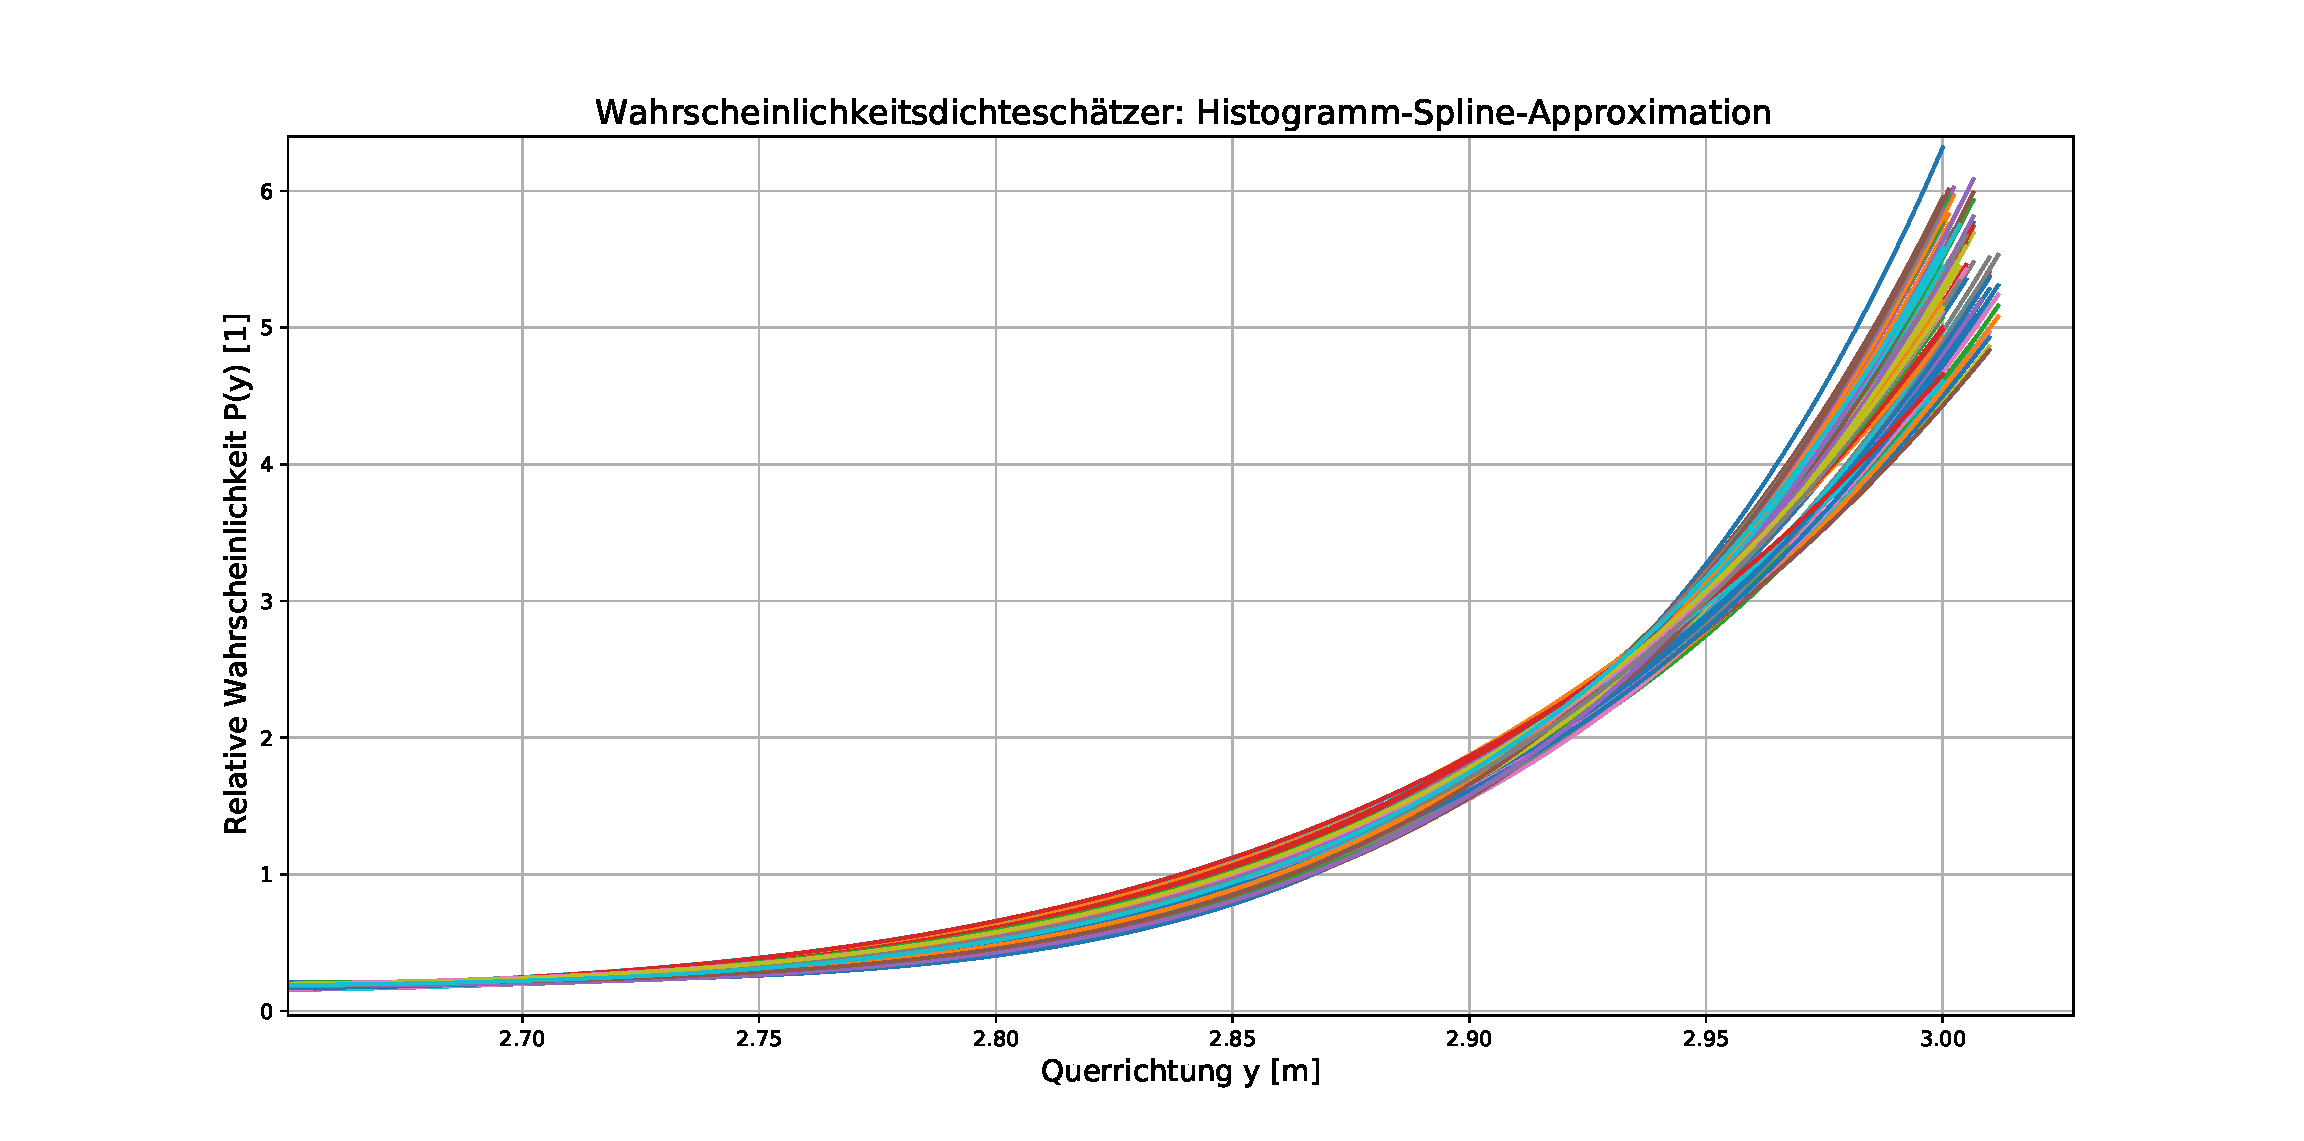
\includegraphics[width=\linewidth,height=0.6\linewidth]{fig/haupt/impl/UeberholvorgangDichtefunktionAusschnitt}
	\caption{Ausschnitt der Dichtefunktionen von synthetisch generierten �berholvorg�ngen}
	\label{img:data:ueberDichtA}
\end{figure}

\begin{figure}[h]
	\centering
	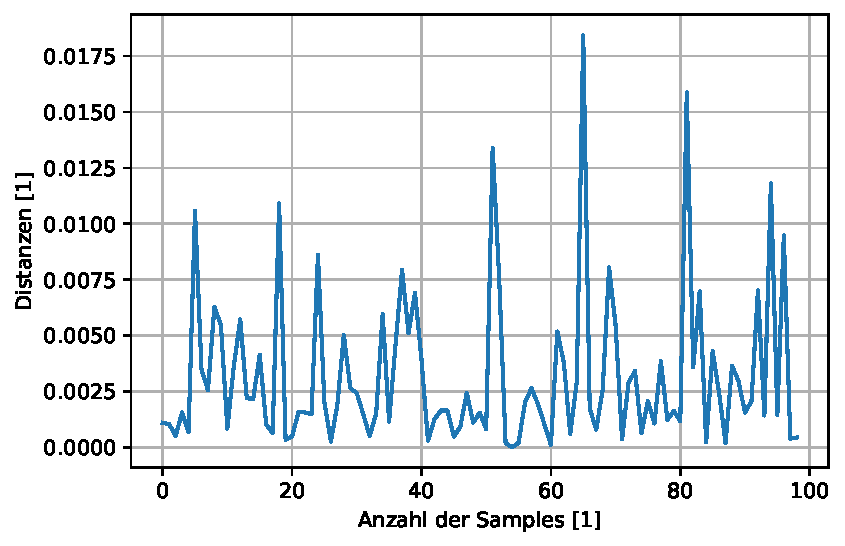
\includegraphics[width=\linewidth,height=0.6\linewidth]{fig/haupt/impl/UeberholKLK}
	\caption{Kullback-Leibler Distanzen f�r Dichtefunktionen der synthetisch generierten �berholvorg�ngen}
	\label{img:data:ueberKLK}
\end{figure}

\begin{figure}
	\centering
	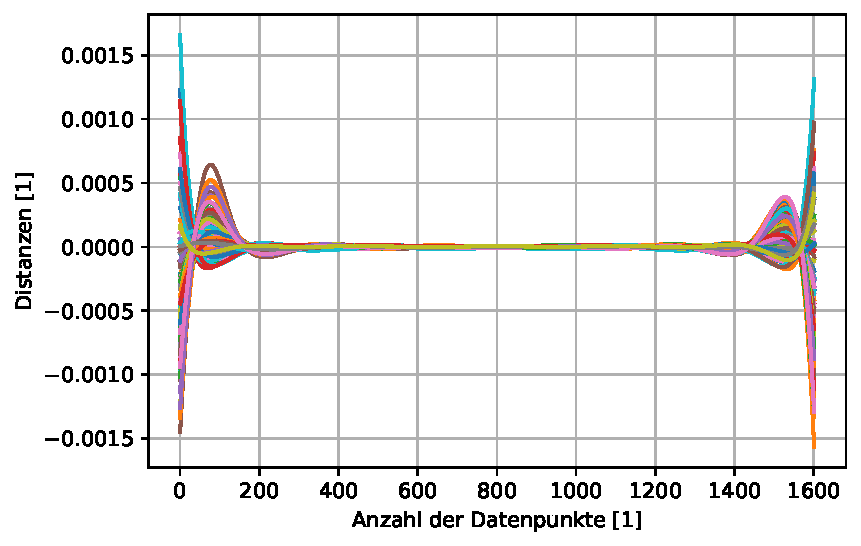
\includegraphics[width=\linewidth,height=0.6\linewidth]{fig/haupt/impl/UeberholKLEinzel}
	\caption{Kullback-Leibler Distanzen f�r Dichtefunktionen der synthetisch generierten �berholvorg�ngen}
	\label{img:data:ueberKLA}
\end{figure}

\FloatBarrier

F�r die Ermittlung der Kullback-Leibler Distanzen wurde, aus den 100 Wahrscheinlichkeitsdichtefunktionen der �berholvorg�nge, eine als Referenz verwendet. In \autoref{img:data:ueberKLK} sind die Kullback-Leibler Distanzen f�r 99 Samples dargestellt. Es ergibt sich stets ein Wert nahe null. Diese Werte sprechen f�r eine hohe �hnlichkeit der Dichtefunktionen.
\\
\\
Die Einzelwerte der Kullback-Leibler Divergenzen sind in \autoref{img:data:ueberKLA} dargestellt. Die Verl�ufe
zeigen eine hohe Varianz f�r den Ein- und Ausschervorgang sowie f�r den �berholvorgang. F�r den Bereich zwischen den Fahrbahnen ergibt sich, wie in den entsprechenden Dichtefunktionen, ein ann�hernd linearer Verlauf. Es sind hierbei, wie im Falle der Sinusfunktionen, verschiedene Punkte mit einer h�heren Konzentration zu beobachten. Diese resultieren ebenso aus der Histogramm-Spline-Approximation.
\\
\\
Es ist zu beachten, dass die Werte hierbei um das zehnfache h�her sind, als die Kullback-Leibler Distanzen der Dichtefunktionen von Sinusfunktionen. Dies l�sst sich anhand der zugrundeliegenden mathematischen Beschreibung erkl�ren. Die Definition einer Sinuskurve ist relativ simpel. Sie besitzt, in Abh�ngigkeit der Variationsparameter, stets einen �hnlichen periodischen Verlauf. Im Gegensatz dazu erfolgt die mathematische Beschreibung eines �berholvorgangs wesentlich komplexer \cite{lit:Schick2020}.
\chapter{Schluss}
\label{sec:schluss}

Im Folgenden wird eine Zusammenfassung der Bachelorarbeit sowie zuk�nftig aufbauende Arbeiten vorgestellt. 

\section{Zusammenfassung}
\label{sec:schluss:zsm}

J�hrlich sterben etwa 1,3 Millionen Menschen bei Verkehrsunf�llen. Die h�ufigste Unfallursache ist hierbei menschliches Fehlverhalten. Aus diesem Grund besitzt das autonome Fahren das Potential, diese auf ein Minimum zu reduzieren. Hierbei werden alle Fahraufgaben vom Fahrzeug �bernommen. Diese m�ssen, um die Sicherheit aller Verkehrsteilnehmer zu gew�hrleisten, jede Situation, im dynamischen Stra�enverkehr, regelkonform bew�ltigen k�nnen. Ebenso m�ssen die dazugeh�rigen System- und Softwarekomponenten ausgiebig getestet werden. Hierzu sind eine gro�e Menge an Daten f�r verschiedenste Fahrsituationen erforderlich, um autonome Fahrzeuge auf diese vorzubereiten. F�r sicherheitskritische Fahrszenarien sind diese, aufgrund ihrer Kritikalit�t, relativ selten vorhanden. Hierbei k�nnen generative Algorithmen verwendet werden, um synthetische Bewegungsdaten f�r diese Szenarien zu generieren.
\\
\\
Die generierten Datens�tze m�ssen, um physikalisch plausible sicherheitskritische Fahrszenarien zu gew�hrleisten, anhand von Evaluierungstechniken, validiert werden. Hierbei wird typischerweise die Wahrscheinlichkeitsdichtefunktion des zugrundeliegenden Datensatzes betrachtet. Im Rahmen dieser Arbeit wurden Evaluierungstechniken f�r derartige Wahrscheinlichkeitsdichtefunktionen untersucht. Dazu wurde, auf Basis einer umfangreichen Literaturrecherche, eine Liste mit existierenden Evaluierungstechniken, erstellt. Hierbei wurden insgesamt ca. 200 Evaluierungstechniken herangezogen.
\\
\\
In einem weiteren Schritt sind die, f�r den Anwendungsfall irrelevanten, Evaluierungstechniken ausgefiltert worden. Die daraus resultierende Liste enthielt 13 hoch relevante Evaluierungstechniken. Diese konnten, auf Basis ihrer mathematischen Beschreibung, in verschiedene Gruppen eingeteilt werden. Daraus entstand eine neuartige Taxonomie von Evaluierungstechniken f�r Wahrscheinlichkeitsdichtefunktionen.
\\
\\
Die einzelnen Evaluierungstechniken wurden detailliert mathematisch beschrieben. In einem weiteren Schritt erfolgte, anhand von definierten Bewertungskriterien, f�r den zugrundeliegenden Anwendungsfall, eine Gegen�berstellung dieser Evaluierungstechniken. Hierbei konnte eine qualitative Empfehlung ausgesprochen werden. Abschlie�end wurde die empfohlene Evaluierungstechnik implementiert und anhand von synthetischen Datens�tzen validiert.

\section{Ausblick}
\label{ec:schluss:ausblick}

Die empfohlene Evaluierungstechnik wird in einer weiterf�hrenden Arbeit verwendet. Hierbei wird die entsprechende Python-Implementierung in die Pipeline eines generativen Algorithmus eingebettet. Dieser generiert synthetische Bewegungsdaten von sicherheitskritische Fahrszenarien. Die Kullback-Leibler Divergenz kann hierbei verwendet werden, um diese Datens�tze, gem�� der zugrundeliegenden Wahrscheinlichkeitsdichtefunktionen, zu validieren.
\\
\\
In diesem Zusammenhang ist ebenso eine st�rkere Pr�fung von anderen, nicht direkt empfohlenen, Evaluierungstechniken denkbar. Speziell die Wasserstein-1 Metrik oder Maximum Mean Discrepancy besitzen eine hohe Qualit�t. Hierbei m�ssen allerdings die entsprechenden Parameter bestimmt werden. Dies ist mit einem weiteren Optimierungsprozess sowie einer vertieften Literaturrecherche verbunden.
\\
\\
Im Rahmen dieser Arbeit wurden ausschlie�lich synthetische Daten analysiert. Diese weisen geringe Messungenauigkeiten auf und besitzen einen festen Wertebereich. Ebenso ist die Auswirkung von Realdaten sowie verschiedenen Wertebereichen auf die Evaluierungstechnik relevant. Schlie�lich soll diese reale sicherheitskritische Szenarien validieren k�nnen.

% % %%%%%% Anhang
\appendix
\chapter{Anhang}
\label{sec:a-kapitel}

\section{Sinusfunktion (Baseline)}
\label{sec:a:sin}


\lstinputlisting[language=Python, caption=Python Code: Sunusfunktion (Baseline), label=lst:a:sin]{fig/haupt/impl/ModellSynthetisierteDatenSinusfunktion.py}
%\caption{Python Code: Sinusfunktion (Baseline)}
%\label{lst:a:sin}

\newpage

\section{�berholvorgang}
\label{sec:a:ueber}


\lstinputlisting[language=python, caption=Python Code: �berholvorgang, label=lst:a:ueber]{fig/haupt/impl/ModellSynthetisierteDatenUeberholvorgang.py}

% % %%%%%% Literaturverzeichnis (darf im deutschen nicht in den Anhang!)
% Einfaches Literaturverzeichnis
%\begin{thebibliography}{XXXX}
\bibitem{doc:stz} Thomas Nonnenmacher, LaTeX Grundlagen - Setzen einer wissenschaftlichen Arbeit Skript, 2008,\url{http://www.stz-softwaretechnik.de}; \textit{(Bei STZ Internetseite unter Publikationen - Skripte) [V.\,2.0 26.02.08]}

\bibitem[Gun04]{doc:gun} Karsten G�nther, LaTeX2 --- Das umfassende Handbuch, Galileo Computing, 2004, \url{http://www.galileocomputing.de/katalog/buecher/titel/gp/titelID-768}; \textit{1. Auflage}
\end{thebibliography}

% Literaturverzeichnis mit Bibtex
%\addcontentsline{toc}{section}{bib/bib}
\bibliography{bib/bib}

% %  Inhalt ENDE %%%%%%%%%%%%%%%%%%%%%%%%%%%%%%%%%%%%%%%%%%%%%%%%%%%%%%%%%%
\end{document}
